\documentclass[12pt,]{book}
\usepackage{lmodern}
\usepackage{setspace}
\setstretch{1.5}
\usepackage{amssymb,amsmath}
\usepackage{ifxetex,ifluatex}
\usepackage{fixltx2e} % provides \textsubscript
\ifnum 0\ifxetex 1\fi\ifluatex 1\fi=0 % if pdftex
  \usepackage[T1]{fontenc}
  \usepackage[utf8]{inputenc}
\else % if luatex or xelatex
  \ifxetex
    \usepackage{mathspec}
  \else
    \usepackage{fontspec}
  \fi
  \defaultfontfeatures{Ligatures=TeX,Scale=MatchLowercase}
\fi
% use upquote if available, for straight quotes in verbatim environments
\IfFileExists{upquote.sty}{\usepackage{upquote}}{}
% use microtype if available
\IfFileExists{microtype.sty}{%
\usepackage{microtype}
\UseMicrotypeSet[protrusion]{basicmath} % disable protrusion for tt fonts
}{}
\usepackage[left=3cm, right=2.5cm, top=3cm, bottom=2.5cm]{geometry}
\usepackage{hyperref}
\hypersetup{unicode=true,
            pdftitle={Inequidades socioeconómicas en relación a los espacios verdes y cobertura de copa: un enfoque espacial aplicado a la ciudad de Cali, Colombia},
            pdfauthor={Presentado para obtar al título de Maestría en SIG (M.Sc. UNIGIS); Universidad de Salzburgo},
            pdfborder={0 0 0},
            breaklinks=true}
\urlstyle{same}  % don't use monospace font for urls
\usepackage{natbib}
\bibliographystyle{apa}
\usepackage{longtable,booktabs}
\usepackage{graphicx,grffile}
\makeatletter
\def\maxwidth{\ifdim\Gin@nat@width>\linewidth\linewidth\else\Gin@nat@width\fi}
\def\maxheight{\ifdim\Gin@nat@height>\textheight\textheight\else\Gin@nat@height\fi}
\makeatother
% Scale images if necessary, so that they will not overflow the page
% margins by default, and it is still possible to overwrite the defaults
% using explicit options in \includegraphics[width, height, ...]{}
\setkeys{Gin}{width=\maxwidth,height=\maxheight,keepaspectratio}
\IfFileExists{parskip.sty}{%
\usepackage{parskip}
}{% else
\setlength{\parindent}{0pt}
\setlength{\parskip}{6pt plus 2pt minus 1pt}
}
\setlength{\emergencystretch}{3em}  % prevent overfull lines
\providecommand{\tightlist}{%
  \setlength{\itemsep}{0pt}\setlength{\parskip}{0pt}}
\setcounter{secnumdepth}{5}
% Redefines (sub)paragraphs to behave more like sections
\ifx\paragraph\undefined\else
\let\oldparagraph\paragraph
\renewcommand{\paragraph}[1]{\oldparagraph{#1}\mbox{}}
\fi
\ifx\subparagraph\undefined\else
\let\oldsubparagraph\subparagraph
\renewcommand{\subparagraph}[1]{\oldsubparagraph{#1}\mbox{}}
\fi

%%% Use protect on footnotes to avoid problems with footnotes in titles
\let\rmarkdownfootnote\footnote%
\def\footnote{\protect\rmarkdownfootnote}

%%% Change title format to be more compact
\usepackage{titling}

% Create subtitle command for use in maketitle
\newcommand{\subtitle}[1]{
  \posttitle{
    \begin{center}\large#1\end{center}
    }
}

\setlength{\droptitle}{-2em}
  \title{Inequidades socioeconómicas en relación a los espacios verdes y
cobertura de copa: un enfoque espacial aplicado a la ciudad de Cali,
Colombia}
  \pretitle{\vspace{\droptitle}\centering\huge}
  \posttitle{\par}
\subtitle{Juan Fernando Correa Caicedo}
  \author{Presentado para obtar al título de Maestría en SIG (M.Sc. UNIGIS) \\ Universidad de Salzburgo}
  \preauthor{\centering\large\emph}
  \postauthor{\par}
  \predate{\centering\large\emph}
  \postdate{\par}
  \date{2018-03-26}

\usepackage{booktabs}
\usepackage{amsthm}
\usepackage[spanish]{babel}
\pagestyle{plain}
\raggedbottom
% \makeatletter
% \def\thm@space@setup{%
%   \thm@preskip=8pt plus 2pt minus 4pt
%   \thm@postskip=\thm@preskip
% }
% \makeatother

\begin{document}
\maketitle

{
\setcounter{tocdepth}{2}
\tableofcontents
}
\listoftables
\listoffigures
\chapter*{Presentación}\label{presentacion}
\addcontentsline{toc}{chapter}{Presentación}

Borrador del texto. Tesis para obtar al el título de master en
Geographical Information Science \& Systems (UNIGIS M.Sc.).

\chapter*{Agradecimientos}\label{agradecimientos}
\addcontentsline{toc}{chapter}{Agradecimientos}

A Elizabeth, Augusto, Ana María y Catalina. Este trabajo fue posible
gracias a su ayuda y cariño.

\chapter*{Resúmen}\label{resumen}
\addcontentsline{toc}{chapter}{Resúmen}

Este proyecto hace uso del censo arbóreo urbano realizado en Santiago de
Cali (Colombia) entre el año 2014 y 2015, de los datos del censo de
población de 2005 y los datos de la estructura ecológica del municipio
del 2014. El propósito es identificar si existen patrones espaciales
estadísticamente significativos que den evidencia de sesgos de los
indicadores de acceso a servicios ambientales del arbolado urbano (AU) y
espacios verdes EV con indicadores socioeconómicos, con el fin de
identificar espacialmente inequidades en el acceso a este tipos de
servicios ecosistémicos.

Para lograrlo se hace uso de modelos de regresión espacial que capturar
fenómenos de agrupamiento y dispersión en los patrones espaciales a
través la inclusión de términos de autocorrelación espacial en la
regresión lineal. Los modelos espaciales de regresión se prueban con dos
tipos de matrices para observar el efecto de la topología de interacción
entre las variables y los resultados del ajuste. Se hace uso de gráficos
estadísticos, mapas de temáticos y de LISA para la identificación de
zonas con niveles deficientes en el acceso.

Los resultados muestran que existen inequidades explicadas por variables
de estatus como el acceso a educación superior, que están además
negativamente correlacionadas con el porcentaje de afrocolombianos en un
sector censal urbano (SU). En relación al acceso a espacios verdes (EV),
no existe evidencia fuerte de que las variable de etnicidad o estatus
sean buenos predictores del acceso. Sin embargo, sí se encontró una alta
concentración del área del EV disponible en muy pocos sectores de la
ciudad.

\chapter*{Abstract}\label{abstract}
\addcontentsline{toc}{chapter}{Abstract}

This project makes use of the urban arboreal census carried out in
Santiago de Cali (Colombia) between 2014 and 2015, the data of the 2005
population census and the data of the ecological structure of the
municipality of 2014. The purpose is to identify if there are spatially
significant patterns that provide evidence of biases in the indicators
of access to environmental services of urban trees (AU) and green spaces
(EV) with socioeconomic indicators, in order to spatially identify
inequities in access to these types of ecosystem services.

To achieve this, spatial regression models are used to capture grouping
and dispersion phenomena in spatial patterns through the inclusion of
terms of spatial autocorrelation in linear regression. The spatial
models are tested with two types of matrices to observe the effect of
the topology in the interaction between the variables and the results of
the adjustment. Statistical graphs, thematic and LISA maps are used to
identify areas with poor levels of access and discuss explanation
related to the causes.

The results show that there are inequities explained by status variables
such as access to higher education, which are also negatively correlated
with the percentage of Afro-Colombians in an urban census sector (SU).
In relation to access to green spaces (EV), there is no strong evidence
that the variables of ethnicity or status are good predictors of access.
However, there was a high concentration of the EV area available in very
few sectors of the city.

\chapter{Introducción}\label{intro}

\section{Antecedentes}\label{antecedentes}

Los árboles son pieza clave de los ecosistemas donde la vida humana ha
prosperado. Son hogar y fuente de alimento de muchas especies
\citep{osorio_vuelo_2009}; forman espacios con condiciones climáticas y
funcionales que complejizan el paisaje y las posibles relaciones entre
los animales \citep{chapman_forests_1998}. Se puede ubicar la década de
los 70 el inicio de un pensamiento ambiental que empieza a ser relevante
en el discurso económico mundial\citep{leff_pensamiento_2012} y que se
consolida con la publicación del Informe Brundtland en 1987. Sin
embargo, las preocupaciones sobre la sostenibilidad y conservación de
los ecosistemas que sustentan la vida en el planeta son relativamente
nuevas en la economía mundial, si la comparamos con la simbiosis entre
árboles y humanos que dan origen a la agricultura y lo convierten en un
elemento simbólico de gran riqueza en el universo religioso y cultural
de la humanidad \citep{leon_calle_arboles_2011}.

El hombre ha materializado espacios urbanos con dimensiones que retan la
imaginación y llevan al límite los sistemas de infraestructura,
abastecimiento y gobernabilidad. En la empresa de consolidar
antroposferas, las ciudades que construimos han desplazados muchos de
los ecosistemas naturales de los territorios que fueron la razón de
escoger justamente esos sitios para el asentamiento, trasladándolos más
allá de los límites de la ciudad, atenuando su presencia/visibilidad en
el mundo de los ciudadanos. Son reemplazados por vías, zonas verdes,
áreas industriales, comerciales y
residenciales\citep{azocar_urbanization_2007}.

Las preocupaciones sobre el crecimiento de la población mundial, su
concentración en centros urbanos y las transformaciones que trae consigo
el proceso de cambio climático, nos obligan a pensar en cómo maximizar
los beneficios que nos brindan las zonas verdes y el bosque urbano como
estrategia para mitigar los efectos negativos de estos procesos
\citep{nesbitt_exploring_2016, laredo_gestion_2011}. A este escenario se
suma trabajos como \citep{nowak_tree_2012} que revelan patrones de
decaimiento estadísticamente significativos del arbolado urbano en 17 de
20 ciudades norteamericanas o \citep{restrepo_incidence_2015} que
reporta la reducción de las condiciones de vitalidad del arbolado del
Valle de Aburra en Colombia derivado de la interacción de causas
naturales y antrópicas, las cuales afectan directa o indirectamente la
fisiología y salud de los árboles en los espacios urbanos.
\citet{nowak_tree_2012} se pregunta si los administradores locales
conocen los cambios que presenta las coberturas arbóreas, puesto que
esta es una representación simple pero confiable (y ampliamente
aceptada) para tasar la extensión de los beneficios derivados de los
bosque urbanos, dado que los servicio que proveen los árboles están
relacionados con la salud y el funcionamiento de sus hojas.

El desarrollo urbano de Cali se fue dando en forma de barrios. Cali
entra al siglo XX con unos de 25000 habitantes y una 100 hectáreas
\citep{vasquez_historia_1990}; en 2005 tiene una población 2200000
habitantes según el Censo de Población del 2005 y una área urbana
12.101.326 hectáreas. Durante todo este siglo experimenta un rápido
crecimiento demográfico, rápida expansión y crecimiento de la vivienda
por las migraciones, causadas en gran medida por los fenómeno de
desplazamiento por conflictos en las áreas rurales y el fortalecimiento
de la industria y el empleo en las ciudad \citep{vasquez_historia_1990}.
Este contexto de crecimiento vertiginoso y no planificado, y las
transformaciones del paisaje e intervención de los ecosistemas coincide
con la necesidades y preocupaciones para garantizar un ambiente
saludable en la ciudad de Cali.

La Organización Mundial de la Salud (OMS) recomienda que una ciudad
tenga un árbol por cada tres habitantes, incluyendo espacios públicos y
privados. Cali debería tener una población arbórea cercana a los 800.000
árboles, pero de acuerdo con los resultados del censo arbóreo de
2014--2015, se han contabilizado cerca de 290.000 árboles solo en el
espacio público. La siembra de 20.000 árboles en la zona urbana, en las
comunas que muestran temperaturas por muy por encima de la media (las
comunas 3, 4, 5, 8 y 13) propuesta en \citep{ciat_identificacion_2015}
contrasta con los 100.000 árboles que tiene como meta en Plan de
Desarrollo Municipal 2016-2019; ambas cifras están lejos de impactar el
déficit arbóreo de 500.000 individuos; urge la reforestación,
\emph{``sin embargo, la ubicación de los sitios de siembra ha sido uno
de los principales inconvenientes del proyecto, ya que no existen zonas
de espacio público adecuadas o disponibles para tal fin.''}
\citep[p.~19]{ciat_identificacion_2015}

En las agendas municipales, a nivel mundial, ha crecido la importancia
de las relaciones y patrones de distribución de los beneficios de áreas
verdes en comparación con la distribución espacial de variables sociales
y económicas como el ingreso, acceso al trabajo, la etnicidad o el
género, con miras a reducir las desigualdades entre los ciudadanos en el
acceso y disfrute de los servicios ambientales. La definición y
valoración de estos beneficios hace uso de medidas como la abundancia,
la cobertura de las copas de los árboles, índices de vegetación,
diferentes distancias a las zonas verdes dentro de un marco alineado con
conceptos como la justicia ambiental, equidad y la sostenibilidad. Estos
indicadores son calculados con datos de censos de población, encuesta de
calidad de vida, censos arbóreos, imágenes satelitales, cartografías y
bases de datos de entidades oficiales y académicas. Los servicios
ambientales tienen cargas y costos de mantenimiento para la
administración y gestión de los recursos y servicios ambientales, lo que
exige que se identifique las zonas, condiciones de los recursos y de la
población para la ejecución de acciones eficaces y eficientes por parte
de los gobiernos y autoridades ambientales.

La distribución espacial equitativa de los beneficios que proveen el
arbolado urbano y las zonas verdes de espacio público, que constituyen
un bien común, financiado y de responsabilidad de las administraciones
municipales\footnote{Así está expresado en las las leyes ambientales que
  dan forma al Sistema Nacional Ambiental, SINA, (LEY 99 DE 1993) y
  reglamentan los planes de desarrollo y de ordenamiento territorial
  (LEY 388 DE 1997), así como la creación de organismos en la estructura
  municipal (Acuerdo 01 de 1996).}, es un componente cuantificable por
medio métodos estadístico y técnicas de análisis espacial con miras a
construir evidencia sobre el disfrute y acceso a los beneficios
ambientales en espacios urbanos y su relación con las condiciones de
vida de la población que habita ese territorio.

\section{Objetivos}\label{objetivos}

\subsection{Objetivo general}\label{objetivo-general}

Identificar y analizar espacialmente la existencia de inequidades en el
acceso a dos servicios ambientales urbanos: el acceso a espacios verdes
y beneficios del arbolado, en relación con variables socioeconómicas de
la población y aspectos relacionados con el uso y estructura física de
las unidades geográficas censales en la zona urbana de Santiago de Cali,
Colombia.

\subsection{Objetivos específicos}\label{objetivos-especificos}

\begin{itemize}
\tightlist
\item
  Generar métricas de acceso a espacios verdes y del nivel de beneficios
  del arbolado urbano.
\item
  Identificar y caracterizar las variables sociales, económicas y
  estructurales para ser relacionadas con acceso a espacios verdes y
  beneficios del arbolado.
\item
  Modelar y evaluar las relaciones entre los diferentes indicadores
  ambientales, sociales, económicos y estructurales.
\end{itemize}

\section{Preguntas de investigación}\label{preguntas-de-investigacion}

Algunas de las preguntas a las que se enfrenta esta investigación son:
¿Cuáles son las zonas que muestran mayores correlaciones negativas entre
las variables sociales y la cobertura de copas o el acceso a zonas
verdes? ¿Es igual tener acceso a un parque pequeño que a uno grande?¿Es
el acceso a servicios del AU y EV una característica local de los
sectores geográficos o se extienden esos beneficios a agrupaciones de
sectores urbanos vecinos? ¿Existen aspectos de tipo urbanístico y de la
estructura de los sectores urbanos que condicionan el desarrollo del
arbolado? ¿Están estos factores de estructura y uso relacionados con las
condiciones de vida de la población? ¿Qué tipo de modelos son los más
apropiados para capturar la dependencia espacial en los datos, si es que
esta existe?

\section{Hipótesis}\label{hipotesis}

\subsection{Beneficios del arbolado
urbano}\label{beneficios-del-arbolado-urbano}

\subsubsection{Hipótesis nula}\label{hipotesis-nula}

La distribución espacial de indicadores socioeconómicos y estructurales
es uniforme o aleatorea con respecto a la distribución de beneficios del
arbolado urbano (AU) en Santiago de Cali\footnote{Una forma de plantear
  la hipótesis nula (\(H_0\)) es negar la que se plantea el investigador
  (hipótesis alternativa \(H_a\)), sin embargo no es la única manera. En
  este caso, lo que se busca es probar que existe un sesgo en la
  distribución de un beneficio ambiental explicado por alguna variable
  socioeconómica o estructural, y que además, este obedece a su patrón
  espacial. Esto se prueba negando la hipótesis nula en primera
  instancia, materializado en los coeficientes de las regresiones y la
  autocorrelación, pues representan una tendencia distinguible de tener
  datos con una distribución aleatoria o uniforme. De ahi que el residuo
  de las regresiones ---lo no explicado---, deba ser ruido gaussiano
  para confiar en las estimaciones de los coeficientes. Al plantear
  \(H0\) \emph{``La distribución espacial de indicadores socioeconómicos
  y estructurales es uniforme o aleatorea con respecto a la distribución
  de beneficios del arbolado urbano (AU) en Santiago de Cali''}, probar
  que esto no es cierto es equivalente a encontrar coeficientes de los
  predictores con significancia y valor influyente y residuos normales
  de varianza constante y no autocorrelacionados espacialmente , por lo
  tanto un buen predictor.}.

\subsubsection{Hipótesis alternas}\label{hipotesis-alternas}

La distribución espacial de indicadores socioeconómicos y estructurales
son un predictor de la distribución de servicios del arbolado urbano
(AU) en Santiago de Cali

\subsubsection{Predicciones}\label{predicciones}

\begin{itemize}
\tightlist
\item
  El patrón espacial de acceso a la educación de la población se
  correlaciona con el acceso a servicios ambientales del AU.
\item
  El patrón espacial de indicadores de discapacidades en la población se
  correlaciona con el acceso a servicios ambientales del AU.
\item
  El patrón espacial de etnicidad se correlaciona con el acceso a
  servicios ambientales del AU.
\item
  El patrón espacial de uso de predios se correlaciona con el acceso a
  servicios ambientales del AU.
\item
  El patrón espacial de características físicas de los predios se
  correlaciona con el acceso a servicios ambientales del AU.
\end{itemize}

\subsection{Acceso a espacios verdes}\label{acceso-a-espacios-verdes}

\subsubsection{Hipótesis nula}\label{hipotesis-nula-1}

La distribución espacial de indicadores socioeconómicos y estructurales
es uniforme o aleatorea con respecto a la distribución del acceso a
espacios verdes (EV) en Santiago de Cali.

\subsubsection{Hipótesis alternas}\label{hipotesis-alternas-1}

La distribución espacial de indicadores socioeconómicos y estructurales
son un predictor de la distribución del acceso a espacios verdes (EV) en
Santiago de Cali.

\subsubsection{Predicciones}\label{predicciones-1}

\begin{itemize}
\tightlist
\item
  El patrón espacial de acceso a la educación de la población se
  correlaciona con el acceso a EV
\item
  El patrón espacial de indicadores de discapacidades en la población se
  correlaciona con el acceso a EV
\item
  El patrón espacial de etnicidad se correlaciona con el acceso a EV
\item
  El patrón espacial de uso de predios se correlaciona con el acceso a
  EV
\item
  El patrón espacial de características físicas de los predios se
  correlaciona con el acceso a EV.
\end{itemize}

\section{Justificación}\label{justificacion}

La inclusión de los componentes ambientales en el ámbito de la
planificación urbana en los planes de ordenamiento territorial que exige
la legislación colombiana\footnote{LEY 388 DE 1997} necesita de la
creación de medidas y la elaboración de análisis sobre su relación con
las condiciones de vida de la población. Las herramientas para
establecer políticas públicas y el seguimiento a las acciones realizadas
por las administraciones municipales deben estar asociadas a
características medibles y objetivas para su implementación. Se espera
que los objetivos y proyectos estén sustentados en estudios científicos
que identifiquen brechas y oportunidades para la intervención y
mejoramiento de los servicios ambientales de los cuales es responsable
el gobierno local. En esta medida este estudio contribuye a la
identificación de relaciones de inequidad en la distribución de los
beneficios que provee el arbolado urbano a través del análisis espacial
de la cobertura arbórea, el acceso a zonas verdes y la distribución de
las variables sociales y económicas de la población. El estudio promete
ser un punto de partida para la identificación de zonas de intervención
del arbolado con el fin de cerrar brechas relacionadas con el desarrollo
sostenible y la justicia ambiental.

Contar con los datos del censo arbóreo de Santiago de Cali permite hacer
análisis de estos beneficios ambientales para la población usando datos
con alta resolución espacial y construir estadísticas a escalas
apropiadas para la intervención y aprovechamiento de los recursos
naturales de la ciudad explotando el potencial que ofrece la información
censal y los conjuntos de datos espaciales de los que dispone la
administración municipal \citep{schwarz_trees_2015}. Los resultados de
esta investigación buscan aportar al debate académico y enriquecer el
proceso de la toma de decisiones y la planificación de la ciudad,
sentando bases técnicas y resultados concretos que el desarrollo de
políticas, proyectos e instrumentos que potencien al árbol y el acceso a
espacio verdes como estrategia para la mejora de la calidad de vida de
los caleños.

\section{Alcance}\label{alcance}

Este trabajo se concentra en describir los patrones espaciales y
establecer la correlación entre métricas para representar los beneficios
del arbolado urbano(AU) y los espacios verdes (EV) con las variables
sociales y económicas de la población e incluye variables de uso de los
predios y características que incluyen factores del contexto urbanístico
de la ciudad buscando estimar la importancia relativa de las relaciones
entre los indicadores ambientales y sociales. El valor explicativo de la
posición en el plano geográfico de las métricas ambientales y
socioeconómicas permite seleccionar los modelos de regresión apropiados
para cuantificar el grado de correlación que existe
\citep{fotheringham_geographically_1998}. El problema comprende la
exploración de las variables sociales, económicas, estructurales y
ambientales, el cálculo de indicadores, la cuantificación de la
correlación, el modelado de la relaciones entre variables y la
identificación de las zonas con acumulación de desigualdades.

El trabajo hace uso del censo arbóreo urbano realizado en Santiago de
Cali (Colombia) entre el año 2014 y 2015, de datos del censo de
población de 2005 y los datos de la estructura ecológica del municipio.
Para ellos se apoya en los aportes de tipo metodológico y estadístico de
la literatura especializada sobre modelos de regresión lineal y modelos
de regresión espacial. Las unidades de análisis espacial son los
sectores censales urbanos (SU) que mantienen una relación geométrica y
de escala similar a la de los barrios, unidad básica del crecimiento y
desarrollo urbano de la ciudad de Cali.

\chapter{Revisión de la literatura}\label{revlit}

\section{Servicios ecosistémicos y su
valoración}\label{servicios-ecosistemicos-y-su-valoracion}

Podemos definir un servicio ambiental o ecosistémico como los beneficios
para la población humana que se derivan directa o indirectamente de los
ecosistemas \citep{bolund_ecosystem_1999}. Los servicios dependen
entonces de los tipos de los ecosistemas con los que cuente el entorno
urbano. \citet{bolund_ecosystem_1999} distinguen 7 tipos de ecosistemas
urbanos: árboles de calle, zonas verdes, bosques urbanos, tierras
cultivadas, humedales, lagos/lagunas, y ríos/arroyos. Todos ellos en
conjunto benefician a la población, y muchos estudios se han encargado
de cuantificar el impacto de estos beneficios, en particular se cuentan
los que se relacionan con los ecosistemas de árboles de calle y las
zonas verdes, como reducción de las temperaturas
\citep{ripoll_condiciones_2010}, reducción de la polución en el aire
\citep{duran_rivera_intercepcion_2009}, secuestro de carbono
\citep{nowak_carbon_2002, mcpherson2013new} , mitigación de los efectos
de calentamiento por gases de efecto invernadero
\citep{laredo_gestion_2011} y mantenimiento del agua en los ecosistemas
o proveyendo alimento como en el caso de los árboles frutales
\citep{konijnendijk_arboles_2005, nolazco_diversidad_2012}, reducción de
los niveles de ruido \citep{bolund_ecosystem_1999}. Otros estudios
argumentan que los beneficios ambientales de los ecosistemas urbanos
pueden medirse directamente en la salud de la población
\citep{bolund_ecosystem_1999, gomez-baggethun_classifying_2013}. Una
forma de clasificar todos estos beneficios e indagar sobre las medidas
usadas las resume \citet{gomez-baggethun_classifying_2013} en una tabla
que reproduzco a continuación (ver tabla \ref{tab:clasf-SerAm}).

\begin{longtable}[]{@{}rrrr@{}}
\caption{\label{tab:clasf-SerAm} Clasificación de servicios ecosistémicos
importantes en zonas urbanas y funciones y componentes subyacentes del
ecosistema}\tabularnewline
\toprule
\begin{minipage}[b]{0.26\columnwidth}\raggedleft\strut
Funciones y componentes\strut
\end{minipage} & \begin{minipage}[b]{0.22\columnwidth}\raggedleft\strut
Servicio Ecosistémico\strut
\end{minipage} & \begin{minipage}[b]{0.19\columnwidth}\raggedleft\strut
Ejemplo\strut
\end{minipage} & \begin{minipage}[b]{0.22\columnwidth}\raggedleft\strut
Ejemplo de indicadores/proxies\strut
\end{minipage}\tabularnewline
\midrule
\endfirsthead
\toprule
\begin{minipage}[b]{0.26\columnwidth}\raggedleft\strut
Funciones y componentes\strut
\end{minipage} & \begin{minipage}[b]{0.22\columnwidth}\raggedleft\strut
Servicio Ecosistémico\strut
\end{minipage} & \begin{minipage}[b]{0.19\columnwidth}\raggedleft\strut
Ejemplo\strut
\end{minipage} & \begin{minipage}[b]{0.22\columnwidth}\raggedleft\strut
Ejemplo de indicadores/proxies\strut
\end{minipage}\tabularnewline
\midrule
\endhead
\begin{minipage}[t]{0.26\columnwidth}\raggedleft\strut
Conversión de energía en plantas comestibles a través de la
fotosíntesis\strut
\end{minipage} & \begin{minipage}[t]{0.22\columnwidth}\raggedleft\strut
Suministro de alimentos\strut
\end{minipage} & \begin{minipage}[t]{0.19\columnwidth}\raggedleft\strut
Hortalizas producidas por lotes urbanos y áreas periurbanas\strut
\end{minipage} & \begin{minipage}[t]{0.22\columnwidth}\raggedleft\strut
Producción de alimentos {[}toneladas/año{]}\strut
\end{minipage}\tabularnewline
\begin{minipage}[t]{0.26\columnwidth}\raggedleft\strut
Percolación y regulación de la escorrentía y la descarga del río\strut
\end{minipage} & \begin{minipage}[t]{0.22\columnwidth}\raggedleft\strut
Regulación del caudal de agua y mitigación de escorrentía\strut
\end{minipage} & \begin{minipage}[t]{0.19\columnwidth}\raggedleft\strut
El suelo y la vegetación percolan el agua durante eventos de
precipitación intensa y / o prolongada\strut
\end{minipage} & \begin{minipage}[t]{0.22\columnwidth}\raggedleft\strut
Capacidad de infiltración del suelo; {[}\%{]} Sellado con respecto a la
superficie permeable {[}ha{]}\strut
\end{minipage}\tabularnewline
\begin{minipage}[t]{0.26\columnwidth}\raggedleft\strut
Fotosíntesis, sombreado y evapotranspiración\strut
\end{minipage} & \begin{minipage}[t]{0.22\columnwidth}\raggedleft\strut
Regulación urbana de la temperatura\strut
\end{minipage} & \begin{minipage}[t]{0.19\columnwidth}\raggedleft\strut
Los árboles y otra vegetación urbana proporcionan sombra, crean humedad
y bloquean el viento\strut
\end{minipage} & \begin{minipage}[t]{0.22\columnwidth}\raggedleft\strut
Índice de área foliar; Disminución de la temperatura {[}° C{]} por
cobertura arbórea{[}m2{]} en parcelas cubierta de árboles\strut
\end{minipage}\tabularnewline
\begin{minipage}[t]{0.26\columnwidth}\raggedleft\strut
Absorción de ondas sonoras por la vegetación y el agua\strut
\end{minipage} & \begin{minipage}[t]{0.22\columnwidth}\raggedleft\strut
Reducción de ruido\strut
\end{minipage} & \begin{minipage}[t]{0.19\columnwidth}\raggedleft\strut
Absorción de ondas sonoras por barreras vegetales, especialmente
vegetación espesa\strut
\end{minipage} & \begin{minipage}[t]{0.22\columnwidth}\raggedleft\strut
Superficie de la hoja {[}m2{]} y distancia a las carreteras {[}m{]};
Reducción de ruido {[}dBA{]} / unidad de vegetación {[}m{]}\strut
\end{minipage}\tabularnewline
\begin{minipage}[t]{0.26\columnwidth}\raggedleft\strut
Filtración y fijación de gases y partículas\strut
\end{minipage} & \begin{minipage}[t]{0.22\columnwidth}\raggedleft\strut
Purificación de aire\strut
\end{minipage} & \begin{minipage}[t]{0.19\columnwidth}\raggedleft\strut
Eliminación y fijación de contaminantes por la vegetación urbana en
hojas, tallos y raíces\strut
\end{minipage} & \begin{minipage}[t]{0.22\columnwidth}\raggedleft\strut
O3, SO2, NO2, CO y PM10 μm removido en {[}toneladas/año{]} multiplicado
por la cobertura arbórea (m2)\strut
\end{minipage}\tabularnewline
\begin{minipage}[t]{0.26\columnwidth}\raggedleft\strut
Barrera física y absorción en energía cinética\strut
\end{minipage} & \begin{minipage}[t]{0.22\columnwidth}\raggedleft\strut
Moderación de los extremos ambientales\strut
\end{minipage} & \begin{minipage}[t]{0.19\columnwidth}\raggedleft\strut
Tormentas, inundaciones y amortiguación de olas por barreras vegetales;
Absorción de calor durante olas de calor severas\strut
\end{minipage} & \begin{minipage}[t]{0.22\columnwidth}\raggedleft\strut
Cubrir la densidad de las barreras de vegetación que separan las áreas
construidas del mar\strut
\end{minipage}\tabularnewline
\begin{minipage}[t]{0.26\columnwidth}\raggedleft\strut
Eliminación o descomposición de nutrientes xénicos\strut
\end{minipage} & \begin{minipage}[t]{0.22\columnwidth}\raggedleft\strut
Tratamiento de desechos\strut
\end{minipage} & \begin{minipage}[t]{0.19\columnwidth}\raggedleft\strut
Filtración de efluentes y fijación de nutrientes por humedales
urbanos\strut
\end{minipage} & \begin{minipage}[t]{0.22\columnwidth}\raggedleft\strut
P, K, Mg y Ca en mgkg-1 en comparación con las normas de calidad del
suelo y del agua\strut
\end{minipage}\tabularnewline
\begin{minipage}[t]{0.26\columnwidth}\raggedleft\strut
Secuestro y fijación de carbono en la fotosíntesis\strut
\end{minipage} & \begin{minipage}[t]{0.22\columnwidth}\raggedleft\strut
Regulación climática\strut
\end{minipage} & \begin{minipage}[t]{0.19\columnwidth}\raggedleft\strut
Secuestro y almacenamiento de carbono por la biomasa de arbustos urbanos
y de tres\strut
\end{minipage} & \begin{minipage}[t]{0.22\columnwidth}\raggedleft\strut
Secuestro de CO2 por árboles (carbono multiplicado por 3.67 para
convertir a CO2)\strut
\end{minipage}\tabularnewline
\begin{minipage}[t]{0.26\columnwidth}\raggedleft\strut
Movimiento de los gametos florales por la biota\strut
\end{minipage} & \begin{minipage}[t]{0.22\columnwidth}\raggedleft\strut
Polinización y dispersión de semillas\strut
\end{minipage} & \begin{minipage}[t]{0.19\columnwidth}\raggedleft\strut
El ecosistema urbano provee hábitat para aves, insectos y
polinizadores\strut
\end{minipage} & \begin{minipage}[t]{0.22\columnwidth}\raggedleft\strut
Diversidad de especies y abundancia de aves y abejorros\strut
\end{minipage}\tabularnewline
\begin{minipage}[t]{0.26\columnwidth}\raggedleft\strut
Ecosistemas con valores recreativos y educativos\strut
\end{minipage} & \begin{minipage}[t]{0.22\columnwidth}\raggedleft\strut
Recreación y desarrollo cognitivo\strut
\end{minipage} & \begin{minipage}[t]{0.19\columnwidth}\raggedleft\strut
Los parques urbanos ofrecen múltiples oportunidades para la recreación,
la meditación y la pedagogía\strut
\end{minipage} & \begin{minipage}[t]{0.22\columnwidth}\raggedleft\strut
Superficie de los espacios públicos verdes {[}ha / habitante (o cada
1000 habitantes){]}\strut
\end{minipage}\tabularnewline
\begin{minipage}[t]{0.26\columnwidth}\raggedleft\strut
Disposición del hábitat para las especies animales\strut
\end{minipage} & \begin{minipage}[t]{0.22\columnwidth}\raggedleft\strut
Avistamiento de animales\strut
\end{minipage} & \begin{minipage}[t]{0.19\columnwidth}\raggedleft\strut
El espacio verde urbano proporciona un hábitat para las aves y otros
animales a los que les gusta ver\strut
\end{minipage} & \begin{minipage}[t]{0.22\columnwidth}\raggedleft\strut
Abundancia de aves, mariposas y otros animales valorados por sus
atributos estéticos\strut
\end{minipage}\tabularnewline
\bottomrule
\end{longtable}

Existen diferentes perspectivas para la evaluación de los servicios
ecosistémicos, en razón de ellos se crean diferentes indicadores,
métodos estadísticos y metodologías para capturar de forma directa o
indirecta los beneficios ambientales.
\citep{gomez-baggethun_classifying_2013} propone 2 tipos de valoración:
la económica y la sociocultural. La valoración sociocultural se enfoca
en la percepción y preferencias de los ciudadanos que están ligadas a
sus costumbres y sistemas de valores. Resalta lo difícil de medir y que
suele ser mejor abordado por instrumentos cualitativos, construcción de
escalas y el uso de narrativas. Un ejemplo de este tipo de trabajos es
\citep{garzon2004vegetacion} se hace referencia a la vegetación en las
ciudades y su incidencia en la vida de las personas, sobre todo en
aquellas comunidades de menores recursos. ``Los árboles están
estrechamente vinculados a la historia de la humanidad; están cargados
de historia, son testigos de varias generaciones, que enlazan su
existencia con la anterior, constituyéndose en documentos vivos de
acontecimientos culturales.'' \citep{ferro_medina_arboles_2010}.
\citep{konijnendijk_arboles_2005} propone además que se valore lo
ambiental, la biodiversidad y sostenibilidad por su carácter fundamental
en la existencia misma del los ecosistemas.

Las metodologías de valoración económica se basan principalmente en
análisis costo beneficios que buscan un aprovechamiento eficiente del
uso del suelo \citep{bolund_ecosystem_1999}. La inversión en el arbolado
urbano y las zonas verdes arroja resultados positivos consistentemente
en la literatura p.e \citep{mcpherson_quantifying_1997} reporta que los
beneficios exceden los costos en ciudades como Chicago y en Adelaide
(Australia) según \citep{killicoat_economic_2002} cada árbol da
beneficios por AUD\$172.

Algunos análisis no se limitan a evaluar el costo de ahorro o el
dispuesto a pagar por la población, para valorar económicamente los
servicios ecosistémicos se basan en modelos biofísicos de los individuos
arbóreos e incluyen variables ambientales, características de lo suelos,
la infraestructura de las zonas y sus habitantes
\citep{nelson_modeling_2009} p.e el modelo UFORE
\citep{nowak_urban_2000} o CBAT \citep{mcpherson_quantifying_1997} , y
que permiten tomar acciones específicas sobre el tipo de vegetación y su
distribución. Sin embargo es importante tener en cuenta que este tipo de
análisis pueden generar incentivos para la conversión indeseable de
ecosistemas urbanos en infraestructura construida, con la consiguiente
pérdida de servicios de los ecosistemas
\citep{gomez-baggethun_classifying_2013}.

La lógica económica de los servicios ecosistémicos puede conducir
también a incentivar procesos paradójicos, como el incrementos de los
precios de las casas y arriendos que derivan en procesos de
gentrificación y desplazamiento de la población que fue beneficiada por
la estrategias de mejoramiento de EV y AU con el propósito de resolver
problemas relacionados con la justicia ambiental.
\citep{wolch_urban_2014}

\section{La perspectiva de la justicia
ambiental}\label{la-perspectiva-de-la-justicia-ambiental}

La justicia ambiental es un concepto que ha evolucionado desde su
aparición en la década de los 1980 a través de organizaciones dedicadas
al activismo ambiental y las redes que ellas forman en conjunto con la
academia, acuñaron conceptos de ecología política como justicia
ambiental, deuda ecológica, epidemiología ambiental, racismo ambiental,
justicia climática, soberanía alimentaria, y responsabilidad ambiental
empresarial, que han sido adoptados también por académicos y por
tomadores de decisiones
\citep{martinez_alier_between_2014, cerda_origen_2011}.

La planeación urbana, las relaciones entre los ciudadanos con los
espacios públicos y con las instituciones que los rigen son la base de
la idea de justicia ambiental propuesta en \citep{low_public_2013}, y
que tiene 3 componentes que la definen: \emph{i)} la justicia
distributiva, que en términos de espacio público se basa asegurar
disponibilidad y acceso equitativo de los espacios y servicios a los
ciudadanos; \emph{ii)} la justicia procedimental o procesal, que se
refieren a los procesos de negociación y toma de decisiones, en concreto
a la percepción de los individuos sobre qué tan justos y equilibrados
son, y por tal motivo más dispuesto a aceptar los resultados aunque no
les favorezca; \emph{iii)} la justicia interaccional, que refiere al
comportamiento y trato de la personas en el espacio público que
configuren comportamiento violento o discriminatorios sobre grupos de la
población. El autor argumenta que las condiciones ambientales provocadas
por los procesos de urbanización y/o contaminación deben analizarse
pensando en satisfacer las tres dimensiones, de lo contrario no es
posible hablar de justicia. \citep{schlosberg_theorising_2013} lleva la
reflexión un poco más lejos, argumentando que las nuevas extensiones de
la justicia ambiental se han movido del discurso a un nuevo dominio,
donde lo natural y ambiental crean las condiciones para la justicia
social.

En \citep{braverman_everybody_2008} se exploran las implicaciones entre
las intervenciones en el arbolado urbano y el control de fenómenos como
el crimen y la gobernabilidad dada las relaciones afectivas y morales de
la población con los árboles. El uso de los árboles puede verse también
una forma de discriminación y de discurso político o tecnología de
gobierno. El uso de zonas verdes y arboles ha sido usado también como
una forma de simbolica de estatus y de poder, y esta afirmación es
consistente que la tendencia en tener distribuciones inequitativas
\citep{braverman_everybody_2008}.

La perspectiva distributiva de la justicia ambiental busca relacionar
entonces métricas usadas para cuantificar los servicios ecosistémicos
con métricas sobre la población y sus condiciones de vida usando
unidades espaciales para caracterizar su comportamiento en el área de
estudio.Típicamente se usan variables ambientales que representan
aspectos biofísicos de los ecosistemas p.e superficie de la hoja, índice
de área foliar, el área de cobertura de la copa o los efectos directos e
indirectos de los ecosistemas sobre variables climáticas p.e temperatura
o humedad, o físico-químicas para representar la composición del suelo y
del aire, o mediciones de la capacidad de secuestrar carbono de los
árboles y la de filtrar agua del suelo.

Los primeros trabajos enmarcados en la justicia ambiental se enfocaron
en la ubicación de plantas de residuos y manejo de desechos
relacionándolos con variables sociales como la etnicidad e indicadores
de segregación racial o en comunidades con bajos ingresos
\citep{heynen_political_2006} y que desarrollan trabajos como
\citep{chakraborty1997exploring, cutter_role_1996}. Posteriormente con
el avance de modelos y tecnologías de la información para la
caracterización de la infraestructura ecológica urbana y la
cuantificación de servicios ambientales se desarrollan metodologías para
establecer relaciones entre distribuciones desiguales adoptando el uso
de la cobertura de copa de los árboles como variable que se consolida
para este tipo de estudios, con variables socioeconómicas principalmente
de raza/etnicidad de la población, que tradicionalmente ha sido una
preocupación en el estudio de las desigualdades sociales
\citep{heynen_political_2006, landry_street_2009, phelps_association_2012, zhou_social_2013, schwarz_trees_2015, watkins_is_2016}.

De los espacios verdes suelen caracterizarse dimensiones sobre el
acceso, su dimensiones físicas, los equipamientos y servicios que
prestan, y si los beneficiarios de son del ámbito local al EV o más
amplio. Igualmente es importante preguntarse por la calidad del parque y
zonas verdes así como los usos, que pueden variar dependiendo de las
comunidades que están disfrutando del parque \citep{kabisch_green_2014}.
El acceso suele ser un concepto complejo de medir, pues el análisis
espacial de los datos arroja variaciones significativas usando
diferentes métricas que proviene de los diferentes conceptos de acceso
usados para su definición \citep{talen_assessing_1998}.

En Cali se han realizado trabajos que caracterizan procesos de
desigualdades entre la población analizando factores como la segregación
racial, brechas salariales, empleabilidad e índices socioeconómicos de
segregación
espacial\citep{arroyo_mina_afrocolombianos_2016, mora_brechas_2014, ceron_indice_2014}.
Aunque todos ellos incluyen una dimensión espacial, en tanto que usan
las comunas como unidades de agregación de las variables
socioeconómicas, su análisis no hace uso de los datos espaciales de los
objetos geográficos, su base teórica son los modelos econométricos de
regresión de mínimos cuadrados o la creación de índices (escalas) para
clasificar las unidades gráficas con la escala p.e
\citep{ceron_indice_2014} que hace uso del escalograma de Guttman, un
método para normalizar las diferentes escalas usando igual número de
rangos discretos y construir un índice acumulativo de todas las
dimensiones. \citet{mora_brechas_2014} estudian la discriminación, tanto
racial como por sexo a través de los modelos econométricos de
Oaxaca-Blinder usado para analizar las diferencias salariales entre dos
grupos usando una función que tiene un componente de discriminación.
Para incluir en la ecuación la procedencia se crean los conglomerados a
priori y se agregan dummies por conglomerado de comunas en la ecuación.
\citet{arroyo_mina_afrocolombianos_2016} evalúan la calidad del empleo
bajo el supuesto de ser buen proxy de la calidad de vida y encuentra que
en Cali existe evidencia de que las poblaciones afro son discriminadas
laboralmente, y que esta discriminación está explicada por el lugar de
residencia. Sin embargo, el método usado es similar al de
\citep{mora_brechas_2014} e inclusive usa los mismo conglomerados para
las variables dummies de la procedencia. Entre los trabajos sobre
segregación racial el de \citep{PACHECO2013121} si hace uso de modelos
de regresión espacial y logra identificar zonas homogéneas con alta
correlación espacial. Además describe los cambios en la segregación
residencial en Cali entre 1993 y 2005 mostrando que la segregación
racial es un fenómeno que se ha mantenido vigente en una ciudad cuya
población afrocolombiana es de 26,2\% del total.

Los estudios que se han llevado a cabo sobre segregación espacial
muestran que la exclusión de grupos étnicos en Cali tiende a coincidir
espacialmente con la segregación de los grupos socioeconómicos de
estratos bajos \citep{ceron_indice_2014}. Tendencia que también se ven
estudios de ciudades norteamericanas
\citep{heynen_political_2006, landry_street_2009, zhou_social_2013, nesbitt_exploring_2016}.

\section{Modelamiento y análisis espacial de variables ambientales y
sociales}\label{modelamiento-y-analisis-espacial-de-variables-ambientales-y-sociales}

Las fuentes de datos con información espacial usada para capturar
variables ambientales relacionadas con la vegetación provienen
principalmente de imágenes
satelitales\citep{landry_street_2009, troy_predicting_2007, vasquez_fuentes_vegetacion_2008, nesbitt_exploring_2016},
imágenes aéreas
\citep{azocar_urbanization_2007, heynen_political_2006, tratalos_urban_2007},
datos de Lidar \citep{shanahan_socio-economic_2014, schwarz_trees_2015}
e inventarios producidos por muestras o censos arbóreos y de espacios
verdes
\citetext{\citealp{comber_using_2008}; \citealp{killicoat_economic_2002}; \citealp[\citet{nowak_carbon_2002}]{nowak_urban_2000}; \citealp{talen_assessing_1998}}.
Las imágenes satelitales son usadas en gran cantidad de los estudios
dadas su creciente disponibilidad y la frecuencia de actualización
---Landsat 8 revisita un mismo punto sobre la superficie de la tierra
cada 16 días con un desfase de 8 días con respecto al satélite Landsat
7---, lo que permite hacer monitoreo y seguimiento a escalas entre los
15 m a 100 m por ancho de píxel. Los indicadores de cobertura calculados
con base en datos de imágenes satelitales son estimados usando la escala
de resolución de la imagen en combinación con el índice de Vegetación de
Diferencia Normalizada (NDVI) que permite diferenciar entre densidad y
tipo de vegetación leñosa o vegetación herbosa
\citep{nesbitt_exploring_2016}.

El uso de inventarios arbores permite estudios más detallados sobre las
características del arbolado y son usados para evaluar la salud y
estructura de los individuos arbóreos y las capacidades específicas de
las especies para proveer servicios ambientales.
\citep{killicoat_economic_2002, nowak_carbon_2002, cowett_methodology_2014}.

Entre los distintos indicadores desarrollados para capturar la extensión
y distribución de los servicios ambientales la cobertura de copas ha
probado ser sensible y eficaz para cuantificar hasta qué punto los
árboles y bosques están proporcionando servicios críticos a los
residentes \citep{nowak_sustaining_2010}. Se usan otros indicadores
además de la cobertura en la literatura, y en muchas ocasiones se
normalizan los valores de las variables ambientales por unidad de área,
usando unidades geográficas definidas e introduciendo métricas sobre la
densidad y cantidad de población beneficiada en el cálculo. De hecho
\citep{cowett_methodology_2014} propone que para analizar con precisión
la distribución espacial de los árboles de las calles y los beneficios
que proporcionan es importante migrar hacia métricas en las que las
especies arbóreas y el tamaño del árbol sean un factor en el cálculo,
pues la mayoría de los servicios de los ecosistemas arbóreos son
proporcionales a la cantidad de área superficial de la hoja; en esta
medida las especies de árboles de mayor estatura típicamente
proporcionan muchos más beneficios que las especies de menor estatura.
Trabajos como \citep{alanis_estructura_2014} usan indicadores ecológicos
de las especies como abundancia, dominancia y frecuencia para construir
índices de importancia para valorar las especies nativas y estructura de
los bosques urbanos, cuya conservación también hace parte de las metas
de manejo del AU \citep{nowak_sustaining_2010}.

La tabla \ref{tab:ind-AU} resume los indicadores para cuantificar
servicios/beneficios y estado de los ecosistemas arbóreos usados en la
literatura revisada.

\begin{longtable}[]{@{}rr@{}}
\caption{\label{tab:ind-AU} Métricas para caracterizar servicios del
AU}\tabularnewline
\toprule
\begin{minipage}[b]{0.57\columnwidth}\raggedleft\strut
Métrica\strut
\end{minipage} & \begin{minipage}[b]{0.31\columnwidth}\raggedleft\strut
Referencia\strut
\end{minipage}\tabularnewline
\midrule
\endfirsthead
\toprule
\begin{minipage}[b]{0.57\columnwidth}\raggedleft\strut
Métrica\strut
\end{minipage} & \begin{minipage}[b]{0.31\columnwidth}\raggedleft\strut
Referencia\strut
\end{minipage}\tabularnewline
\midrule
\endhead
\begin{minipage}[t]{0.57\columnwidth}\raggedleft\strut
Producción de alimentos {[}toneladas/año{]}\strut
\end{minipage} & \begin{minipage}[t]{0.31\columnwidth}\raggedleft\strut
\citep{gomez-baggethun_classifying_2013}\strut
\end{minipage}\tabularnewline
\begin{minipage}[t]{0.57\columnwidth}\raggedleft\strut
Índice de área foliar\strut
\end{minipage} & \begin{minipage}[t]{0.31\columnwidth}\raggedleft\strut
\citep{gomez-baggethun_classifying_2013}\strut
\end{minipage}\tabularnewline
\begin{minipage}[t]{0.57\columnwidth}\raggedleft\strut
Disminución de la temperatura {[}° C{]} por cobertura arbórea{[}m2{]} en
parcelas/sitios cubiertas de árboles\strut
\end{minipage} & \begin{minipage}[t]{0.31\columnwidth}\raggedleft\strut
\citep{gomez-baggethun_classifying_2013}\strut
\end{minipage}\tabularnewline
\begin{minipage}[t]{0.57\columnwidth}\raggedleft\strut
Superficie de la hoja {[}m2{]}\strut
\end{minipage} & \begin{minipage}[t]{0.31\columnwidth}\raggedleft\strut
\citep{gomez-baggethun_classifying_2013}\strut
\end{minipage}\tabularnewline
\begin{minipage}[t]{0.57\columnwidth}\raggedleft\strut
O3, SO2, NO2, CO y PM10 μm removido en {[}toneladas/año{]} multiplicado
por la cobertura arbórea (m2)\strut
\end{minipage} & \begin{minipage}[t]{0.31\columnwidth}\raggedleft\strut
\citep{gomez-baggethun_classifying_2013}\strut
\end{minipage}\tabularnewline
\begin{minipage}[t]{0.57\columnwidth}\raggedleft\strut
Secuestro de CO2 por árbol (carbono multiplicado por 3.67 para convertir
a CO2)\strut
\end{minipage} & \begin{minipage}[t]{0.31\columnwidth}\raggedleft\strut
\citep{gomez-baggethun_classifying_2013}\strut
\end{minipage}\tabularnewline
\begin{minipage}[t]{0.57\columnwidth}\raggedleft\strut
Abundancia (por especie) {[}individuos{]}\strut
\end{minipage} & \begin{minipage}[t]{0.31\columnwidth}\raggedleft\strut
\citep{alanis_estructura_2014}\strut
\end{minipage}\tabularnewline
\begin{minipage}[t]{0.57\columnwidth}\raggedleft\strut
Densidad {[}individuos/m2{]}\strut
\end{minipage} & \begin{minipage}[t]{0.31\columnwidth}\raggedleft\strut
\citep{nowak_sustaining_2010}\strut
\end{minipage}\tabularnewline
\begin{minipage}[t]{0.57\columnwidth}\raggedleft\strut
Cobertura de copa de árbol por persona{[}m2/persona{]}\strut
\end{minipage} & \begin{minipage}[t]{0.31\columnwidth}\raggedleft\strut
\citep{nowak_sustaining_2010}\strut
\end{minipage}\tabularnewline
\begin{minipage}[t]{0.57\columnwidth}\raggedleft\strut
Cobertura de copa de árbol{[}m2{]}\strut
\end{minipage} & \begin{minipage}[t]{0.31\columnwidth}\raggedleft\strut
\citep{nowak_sustaining_2010} y muchos antes también\strut
\end{minipage}\tabularnewline
\begin{minipage}[t]{0.57\columnwidth}\raggedleft\strut
porcentaje de cobertura de copa de árbol en un área\strut
\end{minipage} & \begin{minipage}[t]{0.31\columnwidth}\raggedleft\strut
\citep{nowak_sustaining_2010}\strut
\end{minipage}\tabularnewline
\begin{minipage}[t]{0.57\columnwidth}\raggedleft\strut
Dominancia de una especie en función a la cobertura de copa
{[}m2/ha{]}\strut
\end{minipage} & \begin{minipage}[t]{0.31\columnwidth}\raggedleft\strut
\citep{alanis_estructura_2014}\strut
\end{minipage}\tabularnewline
\begin{minipage}[t]{0.57\columnwidth}\raggedleft\strut
Dominancia relativa de la especie i respecto a la dominancia total\strut
\end{minipage} & \begin{minipage}[t]{0.31\columnwidth}\raggedleft\strut
\citep{alanis_estructura_2014}\strut
\end{minipage}\tabularnewline
\begin{minipage}[t]{0.57\columnwidth}\raggedleft\strut
Frecuencia absoluta de una especie (porcentaje de presencia en los
sitios)\strut
\end{minipage} & \begin{minipage}[t]{0.31\columnwidth}\raggedleft\strut
\citep{alanis_estructura_2014}\strut
\end{minipage}\tabularnewline
\begin{minipage}[t]{0.57\columnwidth}\raggedleft\strut
Abundancia relativa de la especie i respecto a la abundancia total en el
área de estudio\strut
\end{minipage} & \begin{minipage}[t]{0.31\columnwidth}\raggedleft\strut
\citep{alanis_estructura_2014}\strut
\end{minipage}\tabularnewline
\begin{minipage}[t]{0.57\columnwidth}\raggedleft\strut
Árboles por habitante\strut
\end{minipage} & \begin{minipage}[t]{0.31\columnwidth}\raggedleft\strut
POT2014\strut
\end{minipage}\tabularnewline
\begin{minipage}[t]{0.57\columnwidth}\raggedleft\strut
índice de cobertura de copa de árbol alrededor de un punto de
muestreo\strut
\end{minipage} & \begin{minipage}[t]{0.31\columnwidth}\raggedleft\strut
\citep{zhou_social_2013}\strut
\end{minipage}\tabularnewline
\begin{minipage}[t]{0.57\columnwidth}\raggedleft\strut
Porcentaje de cobertura de copa de árbol en servidumbres y espacios
públicos\strut
\end{minipage} & \begin{minipage}[t]{0.31\columnwidth}\raggedleft\strut
\citep{landry_street_2009}\strut
\end{minipage}\tabularnewline
\bottomrule
\end{longtable}

En cuanto a los espacios verdes se valoran típicamente los aspectos
geométricos y el acceso. Los aspectos físicos se caracterizan con
medidas de superficie de los espacios, el porcentaje de área o número de
espacios respecto de las unidades espaciales del análisis; este tipo de
medidas son llamadas por \citep{talen_assessing_1998} la aproximación
contenedor (como el representado en la ecuación \eqref{eq:contenedor}), y
aunque muy extendidas en la literatura para caracterizar acceso a los EV
asumen que los beneficios del espacio verde tiene un impacto local:
\emph{``Sin embargo, si el investigador está seguro de que la esfera de
influencia de un servicio dado se limita a un límite geográfico
específico, puede seguir siendo apropiado el enfoque unidimensional
tradicional de la accesibilidad por medio de conteos por unidad''}
\citep{talen_assessing_1998}. En esta misma línea,
\citep{kabisch_green_2014} asegura que aunque el secuestro de carbono
tiene beneficios a nivel de toda la ciudad, algunos procesos biofísicos
que rigen lo beneficios de los EV ocurren a nivel local. Aunque no es
fácil definir la escala a la que operan los procesos biofísicos, los
beneficiarios de los servicios ambientales son a menudo aquellos que
viven cerca de los EV.

Respecto de las unidades espaciales de agregación de las variables
\citep{cutter_role_1996} encontró que el coeficiente de correlación
tiende a aumentar con el aumento de la escala de las unidades espaciales
de agregación. Para verificar la robustez de las estimaciones de
correlación entre la cantidad de instalaciones tóxicas/desperdicios e
indicadores socioeconómicos \citet{cutter_role_1996} usó pruebas de
hipótesis para probar que tanto explican los indicadores de etnia y de
ingreso la presencia de las instalaciones, agregando los datos a
diferentes escalas de la cartografía censal en EE.UU (condado
\textgreater{} sectores \textgreater{} bloque). Los resultados sugieren
que los sectores y bloques son la escala espacial más apropiada para
evaluar las desigualdades debido a las alta variabilidad de los
indicadores socioeconómicos dentro del condado en comparación con los
sectores y los bloques.

Estos a hallazgos ponen en cuestión la selección del tamaño de la
unidades espaciales del análisis en relación con el área de estudio.
Para el caso de Cali se suele usar las comunas como unidad espacial,
pues es la unidad sobre la que se define la inversión, pero puede no
representar muy bien la escala de los procesos que dominan las
transformaciones en el AU y el acceso a los espacio verdes cuando se
presenta alta variabilidad de los indicadores socioeconómicos y
ambientales.

En esta línea es interesante analizar variables que capturan aspectos
físicos de la estructura del espacio disponible.
\citep{landry_street_2009} relaciona las coberturas con las áreas de los
sectores censales completos y los compara con las áreas de espacio
público sin los lotes de las manzanas de cada sector censal,
introduciendo un indicador espacial que apunta a espacios donde la
responsabilidad es claramente de la instituciones estatales por el
énfasis en el área de jurisdicción para la intervención de la estructura
arbórea y de los espacios verdes (ver tabla \ref{tab:ind-AU}).

Además de las medidas de superficie y sus variantes para caracterizar
los beneficios en una unidad espacial definida, se usan medidas que
relacionan origen destino, como la distancia mínima del centroide de la
unidad espacial al borde del EV más cercano, que proporciona una
estimación fiable de la distancia media desde cualquier punto dentro de
una unidad de análisis. Este método trata a todos los espacios verdes
por igual, independientemente del tamaño y la propiedad
\citep{nesbitt_exploring_2016}.

Para medir el acceso se pueden usar medidas de distancia, que operan
bajo el concepto de costo de viaje. Una forma es calcular la suma de las
distancias desde el centroide de una unidad espacial a \textbf{todos}
los EV, como lo hace la ecuación \eqref{eq:costoviaje} y su variante
\eqref{eq:ncosto} que divide el costo de viaje entre el número de EV
\citep{talen_assessing_1998}. Una alternativa a la suma de distancias es
usar la distancia del centroide al espacio verde más cercano (ecuación
\eqref{eq:mindist}). Otra métrica relevante de acceso es la distancia de
red a través de la estructura de las vías de la ciudad o distancia a
pie, que produce una versión más realista de la experiencia de acceso, y
puede usarse para calcular la distancia mínima promedio de puntos
aleatorios o para cada manzana, por ejemplo, dentro de una unidad de
espacial. Estas métricas exigen marcar los puntos de acceso a las zonas
verdes, tarea que se realiza de forma no automática
\citep{zhou_social_2013}.

\emph{índice contenedor}

\begin{equation}
A^{C}_i =\sum_j{s_j} \;  \; \forall  j \in I
\label{eq:contenedor}
\end{equation}

\emph{costo de viaje}

\begin{equation}
A^{T}_i =\sum_j{d_{ij}} \; 
\label{eq:costoviaje}
\end{equation}

\emph{costo de viaje normalizado}

\begin{equation}
\bar{A}^{T}_i =\sum_j{d_{ij}/N}
\label{eq:ncosto}
\end{equation}

\emph{distancia mínima}

\begin{equation}
A^{M}_i=min\left | d_{ij} \right | 
\label{eq:mindist}
\end{equation}

\emph{índice de accesibilidad a pie}

\begin{equation}
A^{W}= \sum_{\int R_b }{(r_{min}/d_j)}  \;  \; \forall  d_j>0 \; , \; r_{min}<R_b  \;
\label{eq:walkdist}
\end{equation}

El cálculo de estos indicadores e índices de acceso se ha complejizado
con base en recomendación de las agencias ambientales que definen
valores de referencia como la cantidad de EV mínimo disponible ( 2 ha )
en un radio determinado (300m). Esto puede lograrse, por ejemplo, con la
suma de los cocientes entre el radio recomendado y la distancia de un
punto de muestreo dentro de la unidad espacial a cada uno de las EV en
el radio de búsqueda \(R_b\), que suele ser mayor que la distancia de
acceso recomendada \(r_{min}\). Se pueden seleccionar un número de
muestras para cada unidad espacial y sumar o promediar las distancias
obtenidas \citep{zhou_social_2013} o usar el centroide como único punto
(ecuación \eqref{eq:walkdist}). Modificaciones a este índice pueden
incluir el área de la zona verde para cuantificar el acceso y las
características del EV al que se accede \citep{comber_using_2008}.

El tipo de espacios usualmente aceptados como espacio verde urbano en
los estudios incluyen parques y jardines públicos, corredores verdes
(por ejemplo, adyacentes a ríos y canales), reservas naturales locales,
áreas comunes, pequeñas áreas de bosques con sotobosque, sitios de
importancia para la conservación de la naturaleza, áreas de drenaje (es
decir, áreas regularmente inundadas cercanas a los ríos), cementerios,
instalaciones desocupadas cubiertas de vegetación, lagos y humedales,
campos de golf, áreas privadas de asociaciones de propietarios, terrenos
escolares, parcelas y hasta senderos que no son lo suficientemente
grandes para calificar como
parques\citep{nesbitt_exploring_2016, comber_using_2008, kabisch_green_2014, zhou_social_2013}.

La tabla \ref{tab:ind-EV} resume los indicadores usados en la literatura
revisada sobre el acceso a EV.

\begin{longtable}[]{@{}rr@{}}
\caption{\label{tab:ind-EV} Métricas para caracterizar servicios del
EV}\tabularnewline
\toprule
\begin{minipage}[b]{0.57\columnwidth}\raggedleft\strut
Métrica\strut
\end{minipage} & \begin{minipage}[b]{0.31\columnwidth}\raggedleft\strut
Referencia\strut
\end{minipage}\tabularnewline
\midrule
\endfirsthead
\toprule
\begin{minipage}[b]{0.57\columnwidth}\raggedleft\strut
Métrica\strut
\end{minipage} & \begin{minipage}[b]{0.31\columnwidth}\raggedleft\strut
Referencia\strut
\end{minipage}\tabularnewline
\midrule
\endhead
\begin{minipage}[t]{0.57\columnwidth}\raggedleft\strut
Superficie de los espacios públicos verdes {[}ha{]}\strut
\end{minipage} & \begin{minipage}[t]{0.31\columnwidth}\raggedleft\strut
varios\strut
\end{minipage}\tabularnewline
\begin{minipage}[t]{0.57\columnwidth}\raggedleft\strut
Número de instalaciones o servicios contenidos en una unidad dada (por
ejemplo, distrito censal o división político-administrativa)\strut
\end{minipage} & \begin{minipage}[t]{0.31\columnwidth}\raggedleft\strut
\citep{talen_assessing_1998}\strut
\end{minipage}\tabularnewline
\begin{minipage}[t]{0.57\columnwidth}\raggedleft\strut
Potencial de la gravedad\strut
\end{minipage} & \begin{minipage}[t]{0.31\columnwidth}\raggedleft\strut
\citep{talen_assessing_1998}\strut
\end{minipage}\tabularnewline
\begin{minipage}[t]{0.57\columnwidth}\raggedleft\strut
Distancia al EV más cercano{[}m{]}\strut
\end{minipage} & \begin{minipage}[t]{0.31\columnwidth}\raggedleft\strut
\citep{talen_assessing_1998}\strut
\end{minipage}\tabularnewline
\begin{minipage}[t]{0.57\columnwidth}\raggedleft\strut
Coste medio de viaje EV más cercano\strut
\end{minipage} & \begin{minipage}[t]{0.31\columnwidth}\raggedleft\strut
\citep{talen_assessing_1998}\strut
\end{minipage}\tabularnewline
\begin{minipage}[t]{0.57\columnwidth}\raggedleft\strut
Superficie de los espacios públicos verdes por habitante (o cada 1000
habitantes){[}ha/habatiantante{]}\strut
\end{minipage} & \begin{minipage}[t]{0.31\columnwidth}\raggedleft\strut
\strut
\end{minipage}\tabularnewline
\begin{minipage}[t]{0.57\columnwidth}\raggedleft\strut
Cobertura de espacios verdes{[}\%{]}\strut
\end{minipage} & \begin{minipage}[t]{0.31\columnwidth}\raggedleft\strut
varios\strut
\end{minipage}\tabularnewline
\begin{minipage}[t]{0.57\columnwidth}\raggedleft\strut
Distancias entre puntos o nodos en la red de movilidad urbana\strut
\end{minipage} & \begin{minipage}[t]{0.31\columnwidth}\raggedleft\strut
\citep{comber_using_2008}\strut
\end{minipage}\tabularnewline
\begin{minipage}[t]{0.57\columnwidth}\raggedleft\strut
Índice de accesibilidad caminando al parque dentro de un radio\strut
\end{minipage} & \begin{minipage}[t]{0.31\columnwidth}\raggedleft\strut
\citep{zhou_social_2013}\strut
\end{minipage}\tabularnewline
\bottomrule
\end{longtable}

Para la caracterización de las condiciones de vida de la población en
relación con el disfrute a servicios ambientales los indicadores
sociales usados suelen provenir de los censos de población, encuestas de
trabajo o calidad de vida, registros catastrales para el avalúo de
predios y uso de los suelo. La tabla \ref{tab:ind-SoEc} resume algunos
de los indicadores socioeconómicos usados para la evaluación de
inequidades ambientales en la revisión de la literatura realizada.

\begin{longtable}[]{@{}rr@{}}
\caption{\label{tab:ind-SoEc} Métricas para caracterizar aspectos
socioeconómicos de la población y estructura de las unidades espaciales
del EV}\tabularnewline
\toprule
\begin{minipage}[b]{0.57\columnwidth}\raggedleft\strut
Métrica\strut
\end{minipage} & \begin{minipage}[b]{0.31\columnwidth}\raggedleft\strut
Referencia\strut
\end{minipage}\tabularnewline
\midrule
\endfirsthead
\toprule
\begin{minipage}[b]{0.57\columnwidth}\raggedleft\strut
Métrica\strut
\end{minipage} & \begin{minipage}[b]{0.31\columnwidth}\raggedleft\strut
Referencia\strut
\end{minipage}\tabularnewline
\midrule
\endhead
\begin{minipage}[t]{0.57\columnwidth}\raggedleft\strut
Ingreso medio del hogar\strut
\end{minipage} & \begin{minipage}[t]{0.31\columnwidth}\raggedleft\strut
varios\strut
\end{minipage}\tabularnewline
\begin{minipage}[t]{0.57\columnwidth}\raggedleft\strut
Valor medio vivienda ocupada por el propietario\strut
\end{minipage} & \begin{minipage}[t]{0.31\columnwidth}\raggedleft\strut
\citep{cowett_methodology_2014}\strut
\end{minipage}\tabularnewline
\begin{minipage}[t]{0.57\columnwidth}\raggedleft\strut
Porcentaje de viviendas ocupadas\strut
\end{minipage} & \begin{minipage}[t]{0.31\columnwidth}\raggedleft\strut
\citep{cowett_methodology_2014}\strut
\end{minipage}\tabularnewline
\begin{minipage}[t]{0.57\columnwidth}\raggedleft\strut
Porcentaje de población blanca\strut
\end{minipage} & \begin{minipage}[t]{0.31\columnwidth}\raggedleft\strut
\citep{cowett_methodology_2014}\strut
\end{minipage}\tabularnewline
\begin{minipage}[t]{0.57\columnwidth}\raggedleft\strut
Porcentaje de personas con pregrado\strut
\end{minipage} & \begin{minipage}[t]{0.31\columnwidth}\raggedleft\strut
\citep{cowett_methodology_2014}\strut
\end{minipage}\tabularnewline
\begin{minipage}[t]{0.57\columnwidth}\raggedleft\strut
Porcentaje de población afro\strut
\end{minipage} & \begin{minipage}[t]{0.31\columnwidth}\raggedleft\strut
{[}\citet{cowett_methodology_2014}{]}\strut
\end{minipage}\tabularnewline
\begin{minipage}[t]{0.57\columnwidth}\raggedleft\strut
Porcentaje de viviendas arrendadas\strut
\end{minipage} & \begin{minipage}[t]{0.31\columnwidth}\raggedleft\strut
\citep{heynen_political_2006}\strut
\end{minipage}\tabularnewline
\begin{minipage}[t]{0.57\columnwidth}\raggedleft\strut
Densidad de población {[}residentes/ha{]}\strut
\end{minipage} & \begin{minipage}[t]{0.31\columnwidth}\raggedleft\strut
\citep{troy_predicting_2007}\strut
\end{minipage}\tabularnewline
\begin{minipage}[t]{0.57\columnwidth}\raggedleft\strut
Densidad de hogares{[}hogares/ha{]}\strut
\end{minipage} & \begin{minipage}[t]{0.31\columnwidth}\raggedleft\strut
\citep{troy_predicting_2007}\strut
\end{minipage}\tabularnewline
\begin{minipage}[t]{0.57\columnwidth}\raggedleft\strut
Valor medio vivienda ocupada\strut
\end{minipage} & \begin{minipage}[t]{0.31\columnwidth}\raggedleft\strut
\citep{troy_predicting_2007}\strut
\end{minipage}\tabularnewline
\begin{minipage}[t]{0.57\columnwidth}\raggedleft\strut
Porcentaje de viviendas desocupadas\strut
\end{minipage} & \begin{minipage}[t]{0.31\columnwidth}\raggedleft\strut
\citep{troy_predicting_2007}\strut
\end{minipage}\tabularnewline
\begin{minipage}[t]{0.57\columnwidth}\raggedleft\strut
Índice de delincuencia\strut
\end{minipage} & \begin{minipage}[t]{0.31\columnwidth}\raggedleft\strut
\citep{troy_predicting_2007}\strut
\end{minipage}\tabularnewline
\begin{minipage}[t]{0.57\columnwidth}\raggedleft\strut
Porcentaje de viviendas que son viviendas unifamiliares\strut
\end{minipage} & \begin{minipage}[t]{0.31\columnwidth}\raggedleft\strut
\citep{troy_predicting_2007}\strut
\end{minipage}\tabularnewline
\begin{minipage}[t]{0.57\columnwidth}\raggedleft\strut
Tamaño medio del hogar\strut
\end{minipage} & \begin{minipage}[t]{0.31\columnwidth}\raggedleft\strut
\citep{landry_street_2009}\strut
\end{minipage}\tabularnewline
\begin{minipage}[t]{0.57\columnwidth}\raggedleft\strut
Tamaño medio del lote de vivienda\strut
\end{minipage} & \begin{minipage}[t]{0.31\columnwidth}\raggedleft\strut
{[}\citet{shanahan_socio-economic_2014}{]}\strut
\end{minipage}\tabularnewline
\begin{minipage}[t]{0.57\columnwidth}\raggedleft\strut
Densidad de viviendas\strut
\end{minipage} & \begin{minipage}[t]{0.31\columnwidth}\raggedleft\strut
\strut
\end{minipage}\tabularnewline
\begin{minipage}[t]{0.57\columnwidth}\raggedleft\strut
Grados escolares cursados{[}años{]}\strut
\end{minipage} & \begin{minipage}[t]{0.31\columnwidth}\raggedleft\strut
\strut
\end{minipage}\tabularnewline
\begin{minipage}[t]{0.57\columnwidth}\raggedleft\strut
Porcentaje de habitantes con grado profesional\strut
\end{minipage} & \begin{minipage}[t]{0.31\columnwidth}\raggedleft\strut
\citep{nesbitt_exploring_2016}\strut
\end{minipage}\tabularnewline
\begin{minipage}[t]{0.57\columnwidth}\raggedleft\strut
Porcentaje de habitantes con maestría\strut
\end{minipage} & \begin{minipage}[t]{0.31\columnwidth}\raggedleft\strut
\citep{nesbitt_exploring_2016}\strut
\end{minipage}\tabularnewline
\begin{minipage}[t]{0.57\columnwidth}\raggedleft\strut
Edad del barrio\strut
\end{minipage} & \begin{minipage}[t]{0.31\columnwidth}\raggedleft\strut
\strut
\end{minipage}\tabularnewline
\begin{minipage}[t]{0.57\columnwidth}\raggedleft\strut
Edad media de las construcciones\strut
\end{minipage} & \begin{minipage}[t]{0.31\columnwidth}\raggedleft\strut
\citep{zhou_social_2013}\strut
\end{minipage}\tabularnewline
\bottomrule
\end{longtable}

\subsection{Enfoque estadístico}\label{enfoque-estadistico}

El instrumento matemático más popular para establecer relaciones de
dependencia y asociación entre dos variables aleatorias son los índices
de correlación, sin que la relación cuantificada sea necesariamente de
causalidad. La causalidad entre las variables suele ser una apuesta del
investigador y de su conocimiento o intuición sobre los procesos que
dominan las características de las variables aleatorias
\citep{gibbons_mostly_2012}. El coeficiente de correlación de Pearson es
medida usada para caracterizar la fuerza de relaciones lineales,
mientras que coeficientes de correlación como el de Spearman son usados
para encontrar relaciones no necesariamente lineales, pues se calcula
observando si los cambios en una de las variables está relacionado con
incrementos o decrementos de la otra, lo que permite cuantificar
dependencias no lineales. Estos coeficientes son análisis eficaces para
seleccionar variables candidatas a ser incluidos en modelos de
regresión, tanto para seleccionar las variables que tienen relación
fuerte con la variable a predecir, como la independencia lineal de las
variables explicativas, condiciones necesarias para que los métodos de
ajuste de parámetros de los modelos lineales
\citep{gibbons_mostly_2012}. Los coeficientes de correlación, como
estadística de resumen, no pueden reemplazar el examen visual de los
datos y la construcción de relaciones que tengan un fundamento teórico.

Los modelos de regresión lineal son ampliamente usados en la econometría
para construir modelos explicativos con términos que describen
componentes teóricos de los procesos de estudio e inferir el
comportamiento o tendencias en una población con base en una muestra. De
esta forma se pretende cuantificar el cambio de la variable dependiente
(\(y\)) ante aumentos o disminuciones del valor de una de las \(p\)
variables dependientes \(x_j\) donde \(j =1...p\). Cada una de las
observaciones \(i\) , \(i=1...n\) del vector \(X_p\) denominadas
\(x_{ij}\) forman un sistema de ecuaciones lineales donde el parámetro
\(\beta_j\) pesa el aporte explicativo de la variable correspondiente al
estimarlo (ecuación \eqref{eq:lmodel} y \eqref{eq:lmodelM}). Así, los
coeficientes estimados representan la importancia de una variable
independiente en los cambios de la dependiente. Los métodos para
resolver son estimadores de mínimos cuadrados (OLS ordinary
least-square) o de máxima verosimilitud (ML maximum likelihood). Si se
cumple que las variables independientes del modelo y los términos del
error tienen una distribución normal y una varianza constante
(homocedasticidad), entonces el estimador es óptimo entre todos los
estimadores no sesgados lineales y no lineales. Es clave indagar el
cumplimiento de las condiciones de normalidad, en especial en los
residuos. \citep{gibbons_mostly_2012}.

modelo lineal de la i-esima observación

\begin{equation}
y_i=\beta_0+ \beta_1\cdot  x_{i1}+...+\beta_j\cdot  x_{ij}+...+\beta_p\cdot  x_{ip}+e_i
\label{eq:lmodel}
\end{equation}

forma matricial del sistema de ecuaciones a resolver

\begin{equation}
Y_{n\times 1}=X_{n \times p }\mathbf{\beta}_{p\times 1}+e_{(n\times 1)}
\label{eq:lmodelM}
\end{equation}

Estudios como
\citep{heynen_political_2006, vasquez_fuentes_vegetacion_2008} usan
coeficientes de correlación entre los pares de variables ambientales y
socioeconómicas agregadas en unidades censales o administrativas para
luego usar modelos de regresión de lineal con el fin de estimar la
importancia explicativa de las variables a través de la estimación de
los coeficientes.

\citet{tratalos_urban_2007} indaga sobre relaciones entre indicadores
ambientales y el estatus social de los residente en cinco ciudades del
Reino Unido; se usa coeficientes de correlación de Spearman para
seleccionar las variables usadas en un modelo de regresión lineal usando
OLS para probar que los desarrollos urbanos de alta densidad
generalmente se asociaban con un pobre desempeño ambiental, medido por
el tamaño del parche en el espacio verde y los niveles de provisión de
servicios ambientales.

\subsection{Enfoque geoestadístico}\label{enfoque-geoestadistico}

Cuando se analiza los residuos \(e_i\) en un regresión lineal estos
debería ser ruido. Sin embargo si se encuentra que existe algún tipo de
relación de los residuos con la posición de las observaciones \(i\) en
plano geográfico, entonces se puede usar variaciones en el modelo
lineal, que consiste en incluir un término lineal usando la variable
dependiente (modelo autoregresivo SAR, ecuación \eqref{eq:sar}) , las
independientes ( spatial lag o retardo espacial en \(X\) SLX, ecuación
\eqref{eq:slx}), en el error (modelo espacial del error SEM,ecuación
\eqref{eq:sem}) o usando una combinación del modelo de error y
autoregresivo (modelo espacial de Durbin SD,ecuación \eqref{eq:sd}). Todas
estas aproximaciones introducen una matriz de \(W_{n\times n}\), donde
\(n\) es el número de sitios, que captura la influencia de las variables
en relación con su proximidad.

Esto significa que se propone a priori una relación espacial al dar
estructura a \(W\), por ejemplo usando solo valores de 1 (vecino) y 0
(no vecino) a las unidades espaciales contiguas o expresa una relación
global usando una métrica de distancia en los valores de la matriz
\(W\), por ejemplo \(w_{ij}= 1/d_{ij}\) donde \(d_{ij}\) es la distancia
euclidiana entre los centroides de los sitios \(i\) y \(j\) . La idea es
que los vecinos más cercanos influencian más la unidad \(i\), basados en
la primera ley de la geografía o Ley de Tobler\footnote{``Todas las
  cosas están relacionadas entre sí, pero las cosas más próximas en el
  espacio tienen una relación mayor que las distantes.''}
\citep{tobler1970computer}. Este es un supuesto fuerte, y debe ser
coherente con el fenómeno y los datos que lo representan. Justamente con
la matriz \(W\) se calcula el coeficiente de Moran'I
\citep{moran1950notes}, que se usa para probar una asociación global
entre una variable y su posición en el plano. Si los residuos \(e_i\)
muestran una asociación fuerte con la estructura de \(W\) en la prueba
de Moran'I, se sugiere usar alguno de los modelos espaciales
(SAR,SLX,SEM o SD), pues esto significa que no se puede confiar en los
coeficientes estimados por la regresión lineal. Se aduce que \(W\) puede
ayudar a explicar el proceso que se está modelando. De lo contrario es
mejor usar un modelo lineal u otra técnica.
\citep{paez_spatial_2005, kissling_spatial_2008, anselin_under_2002}
hacen una revisión de los procesos espaciales, sus supuesto y los
criterios de ajuste como errores cuadráticos y criterio de información
de Akaike para la selección de un modelo y diseño bien formulado y
ajustado.

Modelo espacial autoregresivo (SAR)

\begin{equation}
Y=X\mathbf{\beta}+\mathbf{\rho}WY+e
\label{eq:sar}
\end{equation}

Modelo de error espacial (SEM)

\begin{equation}
Y=X\mathbf{\beta}+u \\
u=\mathbf{\rho}Wu+e
\label{eq:sem}
\end{equation}

Modelo de retardo espacial en los terminos independiente (SLX)

\begin{equation}
Y=X\mathbf{\beta}+WX\mathbf{\lambda}+e
\label{eq:slx}
\end{equation}

Modelo espacial de Durbin SD

\begin{equation}
Y=X\mathbf{\beta}+\mathbf{\rho}WY+WX\mathbf{\lambda}+e
\label{eq:sd}
\end{equation}

Estudios como
\citep{landry_street_2009, schwarz_trees_2015, zhou_social_2013, shanahan_socio-economic_2014}
hacen uso de modelos autorregresivos y de retardo espacial para explicar
los errores en el modelo lineal y mejorar el ajuste comparando modelos
que relacionan de las variables ambientales(cobertura de copa y acceso a
EV) con indicadores socioeconómicos.

Sin embargo trabajos como {[}\citet{lesage_biggest_2014};
\citet{kissling_spatial_2008};Gibbons \& Overman, 2012{]} hacen una
crítica muy relevante a esta aproximación, y muestran que la inclusión
de los términos de auto regresión (SAR) no aportan mucho, pues existe un
acople entre los estimadores de los coeficientes que le quita peso a la
posibilidad de interpretar los coeficientes como factores del efecto
aislado de uno de las variables explicativas. Además, muestra que el
ajuste no suele ser muy sensible a variaciones en W, lo que derrumba un
poco la idea de importancia de la vecindad definida a priori.
\citep{lesage_biggest_2014} propone que si la meta de usar modelos de
regresión espacial es tener aproximadamente medidas escalares correctas
de resumen de los efectos directos, indirectos y totales sobre la
variable dependiente que surgen de cambios en las variables
explicativas, entonces sí es adecuado el uso de estos modelos
\citep{lesage_biggest_2014}.

Además del uso del análisis de autocorrelación espacial global, se puede
explorar métodos que hacen análisis local de la variabilidad y
sensibilidad de los parámetros usados para las estimaciones OLS. Si no
hay autocorrelación global o ninguna agrupación, todavía podemos
encontrar grupos a nivel local utilizando autocorrelación espacial
local. El hecho de que de la Morán I es una suma de productos cruzados
individuales es explotado por los ``indicadores locales de asociación
espacial'' (LISA) para evaluar la agrupación de las unidades
individuales mediante el cálculo del índice de Moran local para cada
unidad espacial y la evaluación de la significación estadística p-value
para cada sitio i \citep{talen_assessing_1998}. En
\citet{fotheringham_geographically_1998} se muestra que la regresión
geográficamente ponderada (Geographically weighted regression GWR)
produce resultados más informativos con respecto a la variación de
parámetros en el espacio que la simple utilización de los agregados
estadísticos. Estos métodos puede ser utilizado para examinar
visualmente la variabilidad espacial de los resultados de la regresión o
de las variables del estudio a través de una región y así informar sobre
la presencia de no-estacionariedad espacial. La GWR es usada con éxito
en \citep{comber_spatial_2011} para analizar los posibles factores que
pueden ayudar a identificar y caracterizar las dimensiones a tener en
cuenta para mejorar el acceso a la salud.

\subsection{Otras técnicas}\label{otras-tecnicas}

\citep{nesbitt_exploring_2016} investigan la relación de usos de suelo
para establecer diferencias entre las coberturas usando análisis de
varianza (ANOVA). En \citep{kabisch_green_2014} se usa el análisis
cluster para identificar grupos de población con características
socioeconómicas similares y similar acceso a espacios verdes, para luego
analizar si existen diferencias entre la distribución de los espacios
verdes usando el coeficiente de Gini para diferentes grupos de población
definidos en un tipo de análisis de disimilitud.

\chapter{Metodología}\label{meto}

Este trabajo se concentra en indagar en particular sobre la justicia
ambiental distributiva por medio de modelos estadísticos,
geoestadísticos apoyados por el análisis visual de los patrones
espaciales. El motivo principal para hacer uso de este tipo de
aproximación pasa por la identificación de relaciones estadísticamente
significativas entre variables sociales, económicas, estructurales y
ambientales incluyendo la capacidad de detectar agrupaciones de unidades
geográficas con características homogéneas donde intervenir y disminuir
las inequidades en el acceso a servicios ambientales.

Para ello se hará uso de datos del censo arbóreo de 2015\footnote{Desafortunadamente
  los datos del censo arbóreo no están disponibles al público general
  por motivos desconocidos, pues según la legislación Colombiana no
  existe ningún tipo de impedimento ni restricciones de privacidad sobre
  estos datos, que fueron recolectados con dineros públicos. Trabajé con
  una copia a la que tuve acceso por vínculos laborales con la Alcaldía
  de Cali}, el censo de población del 2005\footnote{Disponibles en
  \citep{censo_sistema_dane, dane_cepal_celade_2005, geoportal_DANE}} y
aspectos estructurales del espacio público y privado de las unidades
espaciales de análisis\footnote{Disponibles en
  \citep{geoportal_idesc, noauthor_plan_nodate}}.

\section{Área de estudio}\label{area-de-estudio}

El municipio de Santiago de Cali se encuentra ubicado al suroccidente
colombiano. Es la capital del departamento del Valle del Cauca y es la
tercera ciudad más poblada del país, después de Bogotá y Medellín, con
2.420.114 habitantes según Cali en Cifras 2015\citep{escobar2015cali} .
El municipio tiene un área 561.7 Km2, un área del perímetro urbano 120.4
Km2 (21.4 \%).(Ver figura \ref{fig:ubicacion}).La división
administrativa de la zona urbana son comunas y las comunas se componen
de barrios.

\begin{figure}
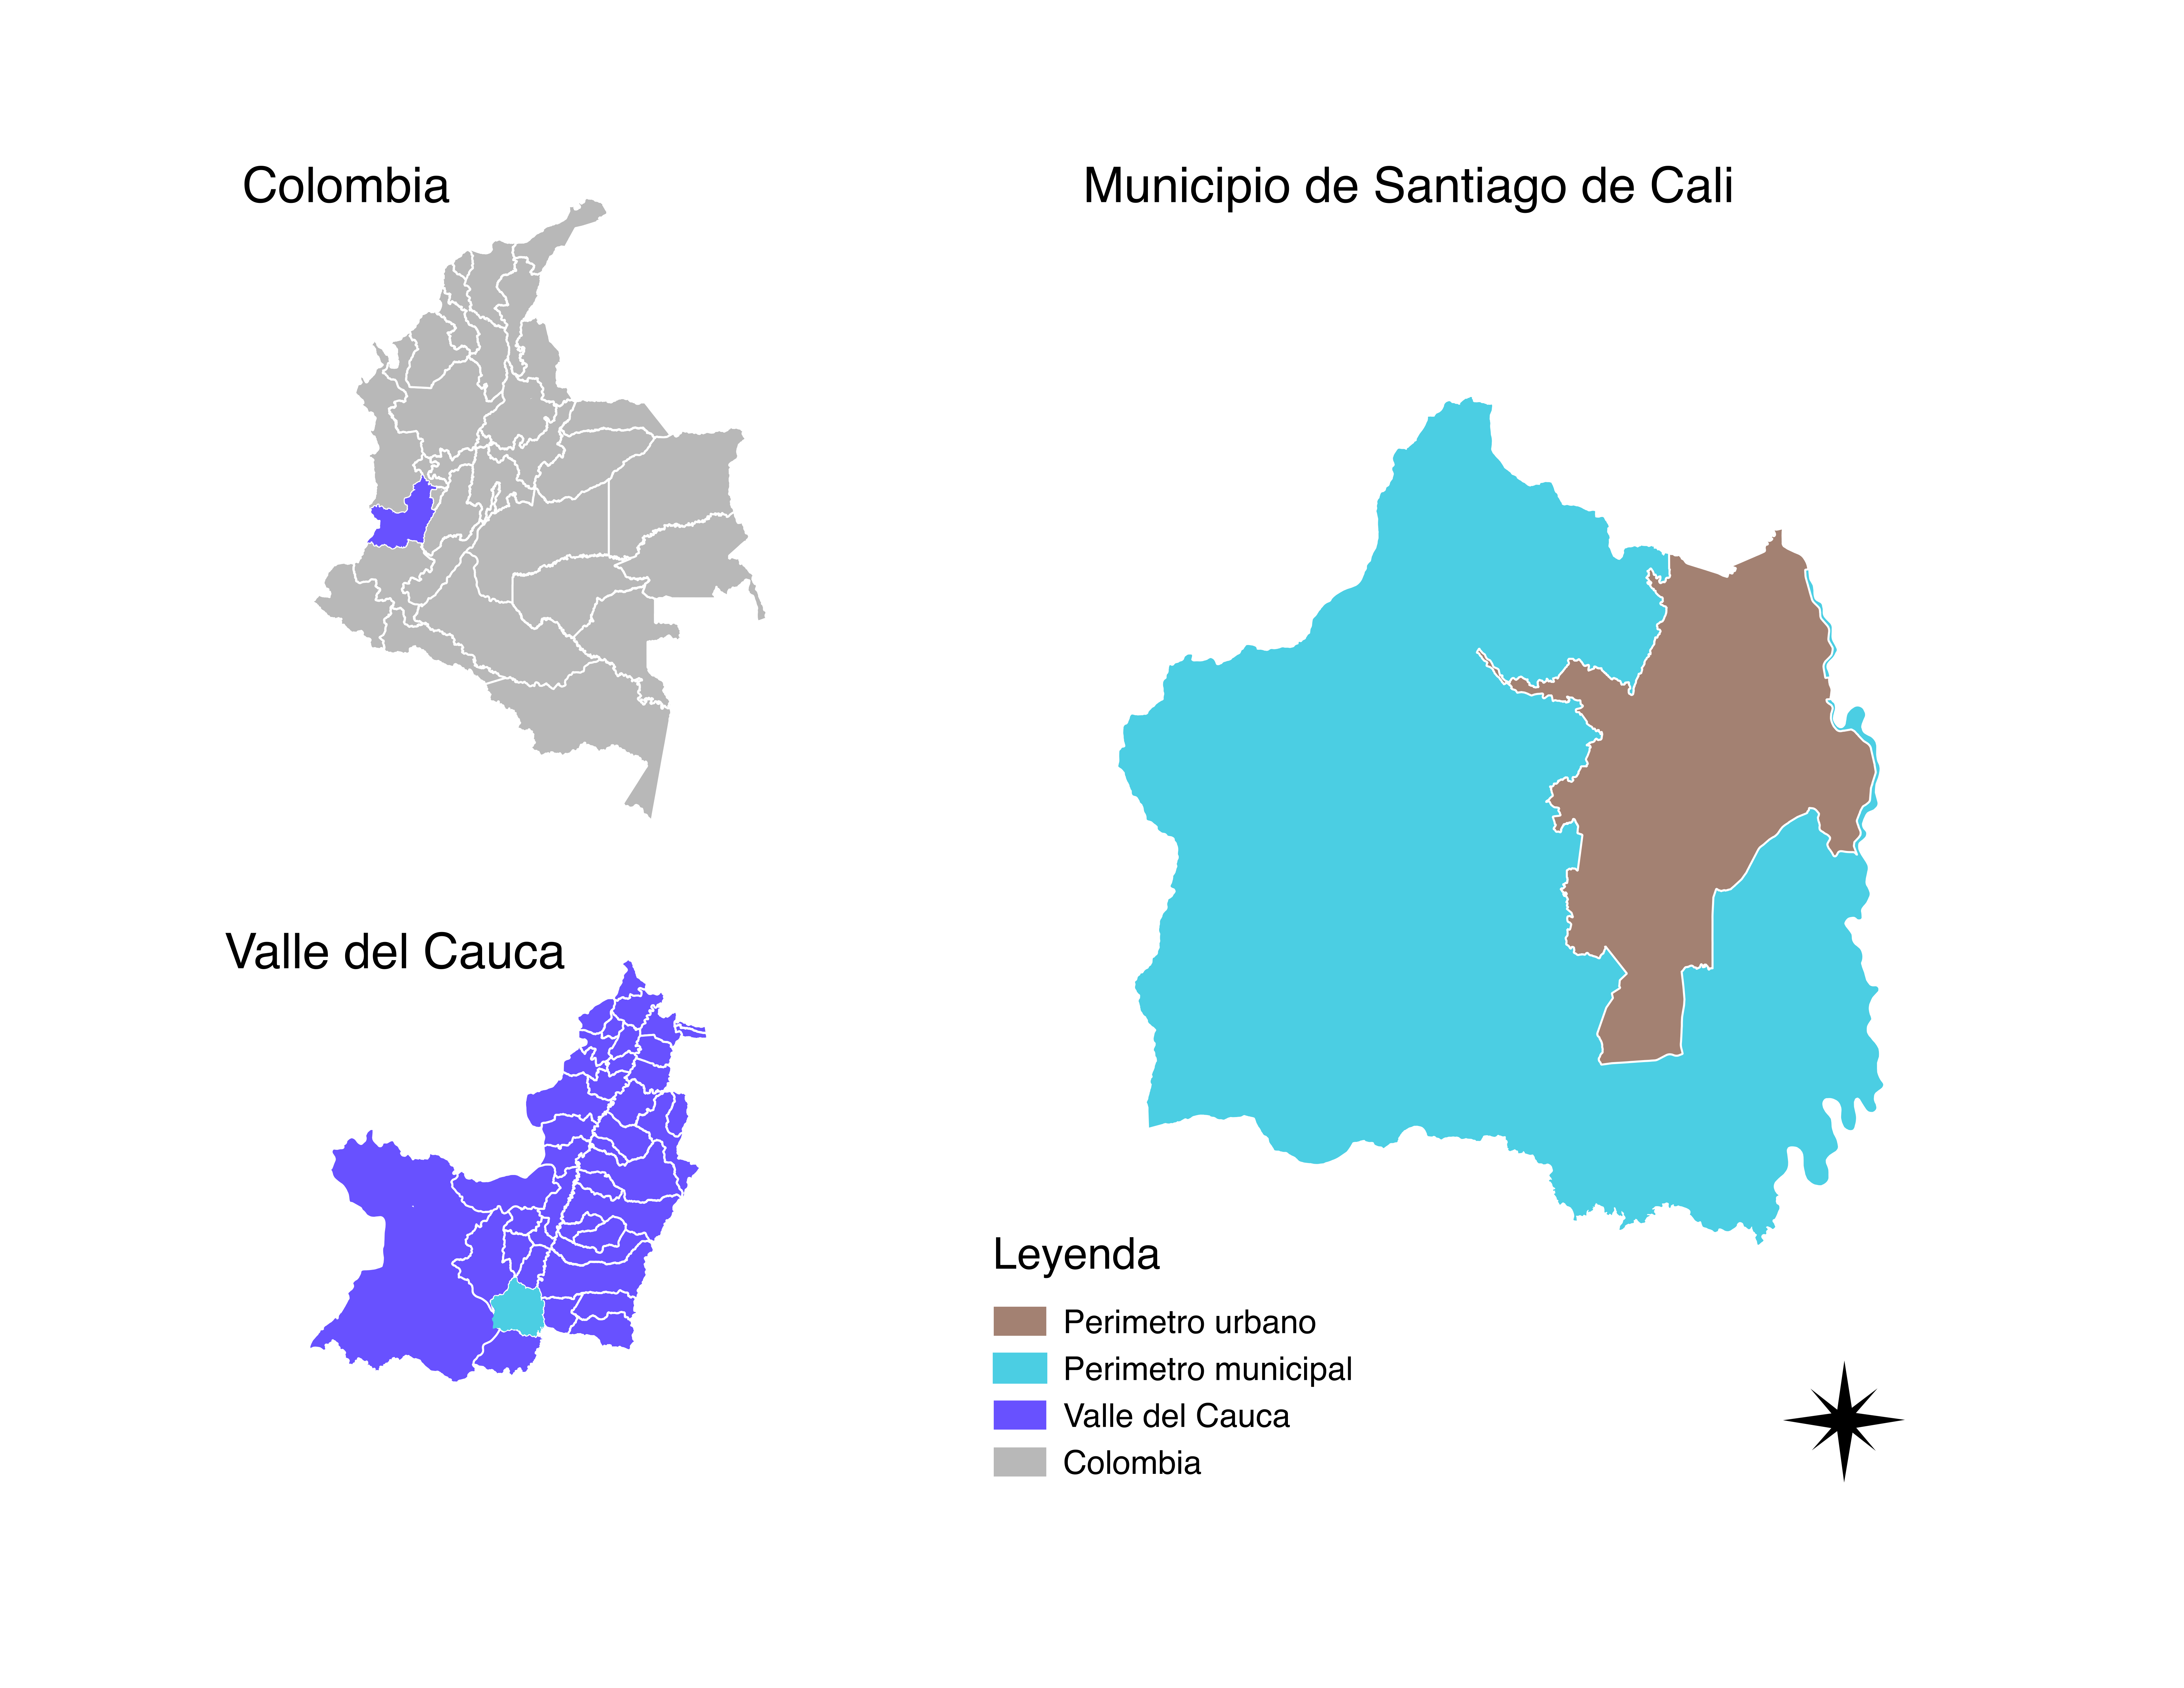
\includegraphics[width=1\linewidth]{QGIS/mapas/ubicacion_cali2} \caption{Área de estudio}\label{fig:ubicacion}
\end{figure}

Santiago de Cali presenta dos zonas topográficas: el valle del río Cauca
hacia el oriente, el terreno más plano donde se ubica el casco urbano, y
la zona de piedemonte hacia el occidente sobre la margen derecha de la
cordillera Occidental. El área urbana limita al oeste y sur con el área
rural del municipio, al este con el río Cauca y los municipios de
Palmira y Candelaria, y al norte con el municipio de Yumbo.

El clima del municipio varía en relación al rango altitudinal que abarca
entre 916 y 1,438 msnm. En la zona plana, se presenta un clima cálido
con características semihúmedas hacia el sur y semiáridas hacia el norte
mientras el piedemonte presenta condiciones de clima templado. La
precipitación anual promedio es de 1.500 mm y la temperatura promedio
anual es de 24 °C aproximadamente \citep{ciat_plan_2015}. La ciudad de
Cali es de clima caliente, donde la sombra y la brisa son bien valoradas
por sus habitantes.

\section{Datos}\label{datos}

\subsection{Datos de registros oficiales del
municipio}\label{datos-de-registros-oficiales-del-municipio}

La cartografía disponible en la Infraestructura de Datos Espaciales de
Santiago de Cali, IDESC \citep{geoportal_idesc}, incluye información
sobre los objetos geográficos naturales, de infraestructura urbana,
límites y divisiones político administrativas y la clasificación de
predios en cuanto a espacio público disponibles en coordenadas planas
del sistema \citep{noauthor_magna-sirgas-cali_nodate}. Además está la
base de datos geográfica del Plan de Ordenamiento territorial de Cali
2014, POT2014\footnote{Toda la información del POT2014 se encuentra en
  la web de la Alcaldía y puede descargarse como archivo GDB compatible
  con ArcGIS 10.4 o consumirse de Geoserver de IDESC como WFS o mapas en
  formato pdf del acuerdo}. Del POT2014 se seleccionaron conjuntos de
datos de equipamientos y espacio público contenido en la estructura
ecológica complementaria (ECC) que incluye cementerios, universidades,
EV de acceso no restringido aunque algunos sea predios privados
contenidos en EEC. De la IDESC se seleccionó la capa de barrios, espacio
público, humedales, ríos y corredores ambientales disponibles vía WFS.
La capa de manzanas es necesaria para refinar las capas de espacio verde
y poder calcular el área de calle , área privada y otras métricas sobre
la estructura de cada sector sector censal y que servirán como criterios
para la selección de sectores urbanos a incluir en los análisis de
regresión.

En la figura \ref{fig:capas-idesc} se muestra un mapa con las capas
seleccionadas para el realizar el procesamiento y los análisis.

\begin{figure}
\includegraphics[width=1\linewidth]{QGIS/mapas/capas_analisis} \caption{Capas usadas para el procesamiento de los espacios verdes y las características de las manzanas}\label{fig:capas-idesc}
\end{figure}

\subsection{El censo arbóreo}\label{el-censo-arboreo}

En el año 2015 la ciudad de Santiago de Cali (Colombia) concretó la
realización de un censo arbóreo que dejó como resultado una base de
datos de aproximadamente 290.000 individuos censados. Los datos dan
cuenta de la identificación de especies, sus características
dasométricas, de emplazamiento y estado fitosanitario. Estos datos
constituyen un insumo fundamental para para la caracterización de los
beneficios y cargas que supone el mantenimiento y desarrollo del
arbolado urbano. De hecho, su realización ocurre en el marco del proceso
de formulación del plan silvicultura urbana o estatuto arbóreo\footnote{El
  proyecto de censo arbóreo se formuló en dos fases; la primera se
  ejecutó mediante convenio No 095 de 2013 entre la CVC y la Universidad
  Autónoma de Occidente, y la segunda fase mediante convenio No 049 de
  2014 entre las mismas entidades. Los datos no se encuentran publicados
  y fueron solicitados mediante un derecho de petición.} (Acuerdo 0335
de 2013). Las variables biofísicas recolectadas y la georeferenciación
de los individuos permite agregar las características del arbolado a
diferentes escalas de las unidades administrativas p.e divisiones
censales, para identificar y caracterizar su distribución espacial y
correlación con variables sociales o/y económicas. ALgunas de las
variables incluidas en el censo se resumen en la tabla \ref{tab:vars-AU}
y en la tabla \ref{tab:datos-ca2015}.

\begin{longtable}[]{@{}rr@{}}
\caption{\label{tab:vars-AU} Variables para caracterizar el
AU}\tabularnewline
\toprule
\begin{minipage}[b]{0.09\columnwidth}\raggedleft\strut
variable\strut
\end{minipage} & \begin{minipage}[b]{0.38\columnwidth}\raggedleft\strut
\{valores\}{[}unidades{]}\strut
\end{minipage}\tabularnewline
\midrule
\endfirsthead
\toprule
\begin{minipage}[b]{0.09\columnwidth}\raggedleft\strut
variable\strut
\end{minipage} & \begin{minipage}[b]{0.38\columnwidth}\raggedleft\strut
\{valores\}{[}unidades{]}\strut
\end{minipage}\tabularnewline
\midrule
\endhead
\begin{minipage}[t]{0.09\columnwidth}\raggedleft\strut
id\_arbol\strut
\end{minipage} & \begin{minipage}[t]{0.38\columnwidth}\raggedleft\strut
número entero único\strut
\end{minipage}\tabularnewline
\begin{minipage}[t]{0.09\columnwidth}\raggedleft\strut
diametro copa\strut
\end{minipage} & \begin{minipage}[t]{0.38\columnwidth}\raggedleft\strut
{[}m\textsuperscript{2}{]}\strut
\end{minipage}\tabularnewline
\begin{minipage}[t]{0.09\columnwidth}\raggedleft\strut
altura arbol\strut
\end{minipage} & \begin{minipage}[t]{0.38\columnwidth}\raggedleft\strut
{[}m{]}\strut
\end{minipage}\tabularnewline
\begin{minipage}[t]{0.09\columnwidth}\raggedleft\strut
vitalidad\strut
\end{minipage} & \begin{minipage}[t]{0.38\columnwidth}\raggedleft\strut
\{Regular, Sano, Seco, Muerto\}\strut
\end{minipage}\tabularnewline
\begin{minipage}[t]{0.09\columnwidth}\raggedleft\strut
edad\strut
\end{minipage} & \begin{minipage}[t]{0.38\columnwidth}\raggedleft\strut
\{Juvenil, Maduro, Longevo\}\strut
\end{minipage}\tabularnewline
\begin{minipage}[t]{0.09\columnwidth}\raggedleft\strut
emplazamiento\strut
\end{minipage} & \begin{minipage}[t]{0.38\columnwidth}\raggedleft\strut
\{Anden, Bahias de estacionamiento, Bulevares, Corredor Ferreo,
Escenario deportivo y/o Cultural, Glorieta, Parque Urbano, Paseos,
Plaza, Plazoleta, Ronda de rios, Rondas de canales, Separador
Vial\}\strut
\end{minipage}\tabularnewline
\begin{minipage}[t]{0.09\columnwidth}\raggedleft\strut
vegetación\strut
\end{minipage} & \begin{minipage}[t]{0.38\columnwidth}\raggedleft\strut
\{Arbol, Arbusto, Bambu, Muerto, Palma, Planta arbustiva, Seco\}\strut
\end{minipage}\tabularnewline
\begin{minipage}[t]{0.09\columnwidth}\raggedleft\strut
Este\strut
\end{minipage} & \begin{minipage}[t]{0.38\columnwidth}\raggedleft\strut
{[}m{]} MAGNA - SIRGAS-CALI\strut
\end{minipage}\tabularnewline
\begin{minipage}[t]{0.09\columnwidth}\raggedleft\strut
Norte\strut
\end{minipage} & \begin{minipage}[t]{0.38\columnwidth}\raggedleft\strut
{[}m{]} MAGNA - SIRGAS-CALI\strut
\end{minipage}\tabularnewline
\bottomrule
\end{longtable}

\begin{figure}
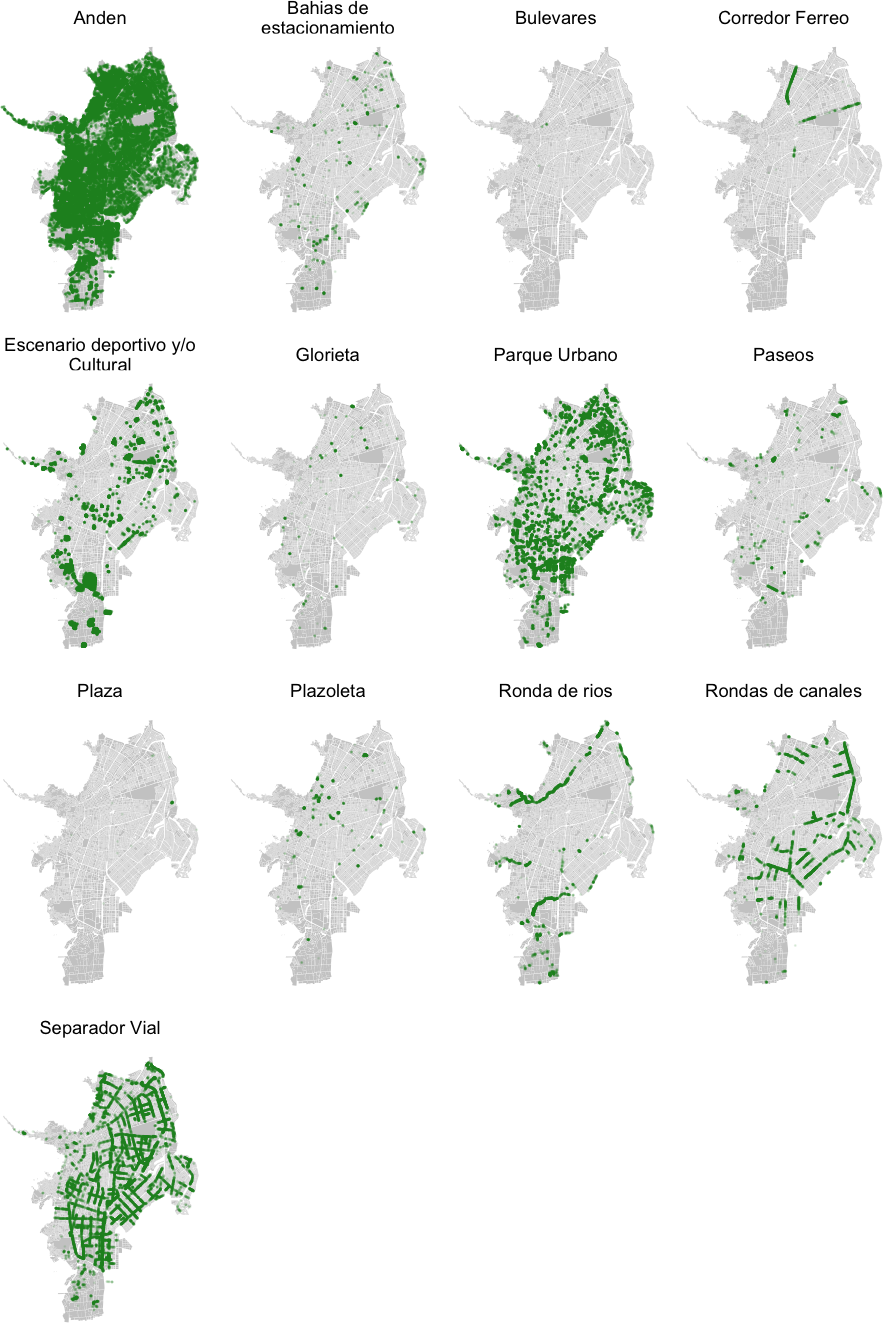
\includegraphics[width=1\linewidth]{tesis-unigis_files/figure-latex/au-geo-emp-1} \caption{Small multiples de los individuos arbóreos por emplazamiento}\label{fig:au-geo-emp}
\end{figure}

\begin{table}

\caption{\label{tab:datos-ca2015}Muestra de los datos del censo arbóreo}
\centering
\begin{tabular}[t]{r|r|r|r|r|r}
\hline
id & vegetacion & edad & emplazamiento & diametro\_copa & altura\_arbol\\
\hline
0199G41070768 & Arbol & Maduro & Ronda de rios & 12 & 11\\
\hline
0199G41070769 & Arbol & Maduro & Ronda de rios & 7 & 8\\
\hline
0199G41070770 & Arbol & Maduro & Ronda de rios & 5 & 3\\
\hline
0199G41070771 & Arbol & Maduro & Ronda de rios & 6 & 7\\
\hline
0199G41070772 & Arbol & Maduro & Ronda de rios & 9 & 8\\
\hline
0199G41070773 & Arbol & Maduro & Ronda de rios & 10 & 7\\
\hline
\end{tabular}
\end{table}

Existe una diferencia de 10 años entre censo de población de 2005 y el
censo arbóreo de la ciudad de Cali. Aunque esto pueda parecer una
situación que reduce la legitimidad de los resultados que se hallen en
este estudio, autores como \citet{boone2010landscape} y
\citet{schwarz_trees_2015} reconocen que los paisajes que vemos hoy son
legados de patrones de consumo pasados, y que en el caso de la
vegetación urbana tratamos con organismos de larga vida que pueden
tardar mucho tiempo en establecerse y crecer. En contraste, la
estructura social de las ciudades puede cambiar más rápidamente.

Una apuesta para reducir la brecha es la exclusión de los árboles
jóvenes del inventario, que posiblemente no estaban ahí en 2005. Aunque
no conocemos las tasa anual de tala de árboles en la ciudad, y dado es
posible que una parte importante de los árboles jóvenes haya reemplazado
a los que fueron talados, no parece realista mantener el inventario
entero.

En general toda la vegetación aporta beneficios ambientales a los
habitantes, en este estudio descartamos la vegetación arbustiva y los
árboles, palmas y bambú de menos de 1.9 m de altura para
circunscribirnos a los individuos más desarrollados.

Una vez aplicado este filtro contamos con 203112 individuos.

\subsection{El censo de población}\label{el-censo-de-poblacion}

El último censo de población en Colombia se realizó en el año 2005, y
los datos se pueden consultar y agregar en las diferentes unidades
censales (sector, sección, manzana) usando una sistema de consulta web
de censos Redatam\footnote{El sistema de consulta es el
  \citep{cepal_redatam_nodate}, que se puede acceder directamente desde
  \citep{dane_cepal_celade_2005} y en la página web del
  \href{http://www.dane.gov.co/index.php/estadisticas-por-tema/demografia-y-poblacion/censo-general-2005-1}{DANE}
  dónde está organizada la documentación metodológica y otros servicios
  del censo.}. Estos datos sirven para caracterizar la población con
base en indicadores y rasgos de las personas, aspectos sobre el uso del
suelo y los tipos de vivienda. Las variables disponibles para el
análisis están resumidas en las tablas \ref{tab:vars-poblacion} y
\ref{tab:vars-vivienda}.

El otro componente de los datos es la cartografía censal del DANE
\citep{geoportal_DANE} disponible para las diferentes unidades
espaciales de agregación en el sistema de coordenadas WGS84. Para el
análisis se tiene en cuenta todos las unidades censales que se
interceptan con el perímetro urbano disponible en la IDESC, pues el
censo arbóreo se limitó al este perímetro.(ver figura
\ref{fig:su-periurbano})

\begin{longtable}[]{@{}rr@{}}
\caption{\label{tab:vars-poblacion} Variables sobre la
población}\tabularnewline
\toprule
\begin{minipage}[b]{0.09\columnwidth}\raggedleft\strut
variable\strut
\end{minipage} & \begin{minipage}[b]{0.38\columnwidth}\raggedleft\strut
\{valores\}{[}unidades{]}\strut
\end{minipage}\tabularnewline
\midrule
\endfirsthead
\toprule
\begin{minipage}[b]{0.09\columnwidth}\raggedleft\strut
variable\strut
\end{minipage} & \begin{minipage}[b]{0.38\columnwidth}\raggedleft\strut
\{valores\}{[}unidades{]}\strut
\end{minipage}\tabularnewline
\midrule
\endhead
\begin{minipage}[t]{0.09\columnwidth}\raggedleft\strut
Pertenencia Étnica\strut
\end{minipage} & \begin{minipage}[t]{0.38\columnwidth}\raggedleft\strut
{[}personas{]}\{indígenas, ROM, gitanos, raizales del Archipiélago de
San Andrés, Providencia y Santa Catalina, palenqueros de San Basilio,
afrocolombianos\}\strut
\end{minipage}\tabularnewline
\begin{minipage}[t]{0.09\columnwidth}\raggedleft\strut
Con alguna limitación\strut
\end{minipage} & \begin{minipage}[t]{0.38\columnwidth}\raggedleft\strut
{[}personas{]}\{sí,no\}\strut
\end{minipage}\tabularnewline
\begin{minipage}[t]{0.09\columnwidth}\raggedleft\strut
Con estudios superior o postgrado\strut
\end{minipage} & \begin{minipage}[t]{0.38\columnwidth}\raggedleft\strut
{[}personas{]}\strut
\end{minipage}\tabularnewline
\begin{minipage}[t]{0.09\columnwidth}\raggedleft\strut
Ningún estudio\strut
\end{minipage} & \begin{minipage}[t]{0.38\columnwidth}\raggedleft\strut
{[}personas{]}\strut
\end{minipage}\tabularnewline
\bottomrule
\end{longtable}

\begin{figure}
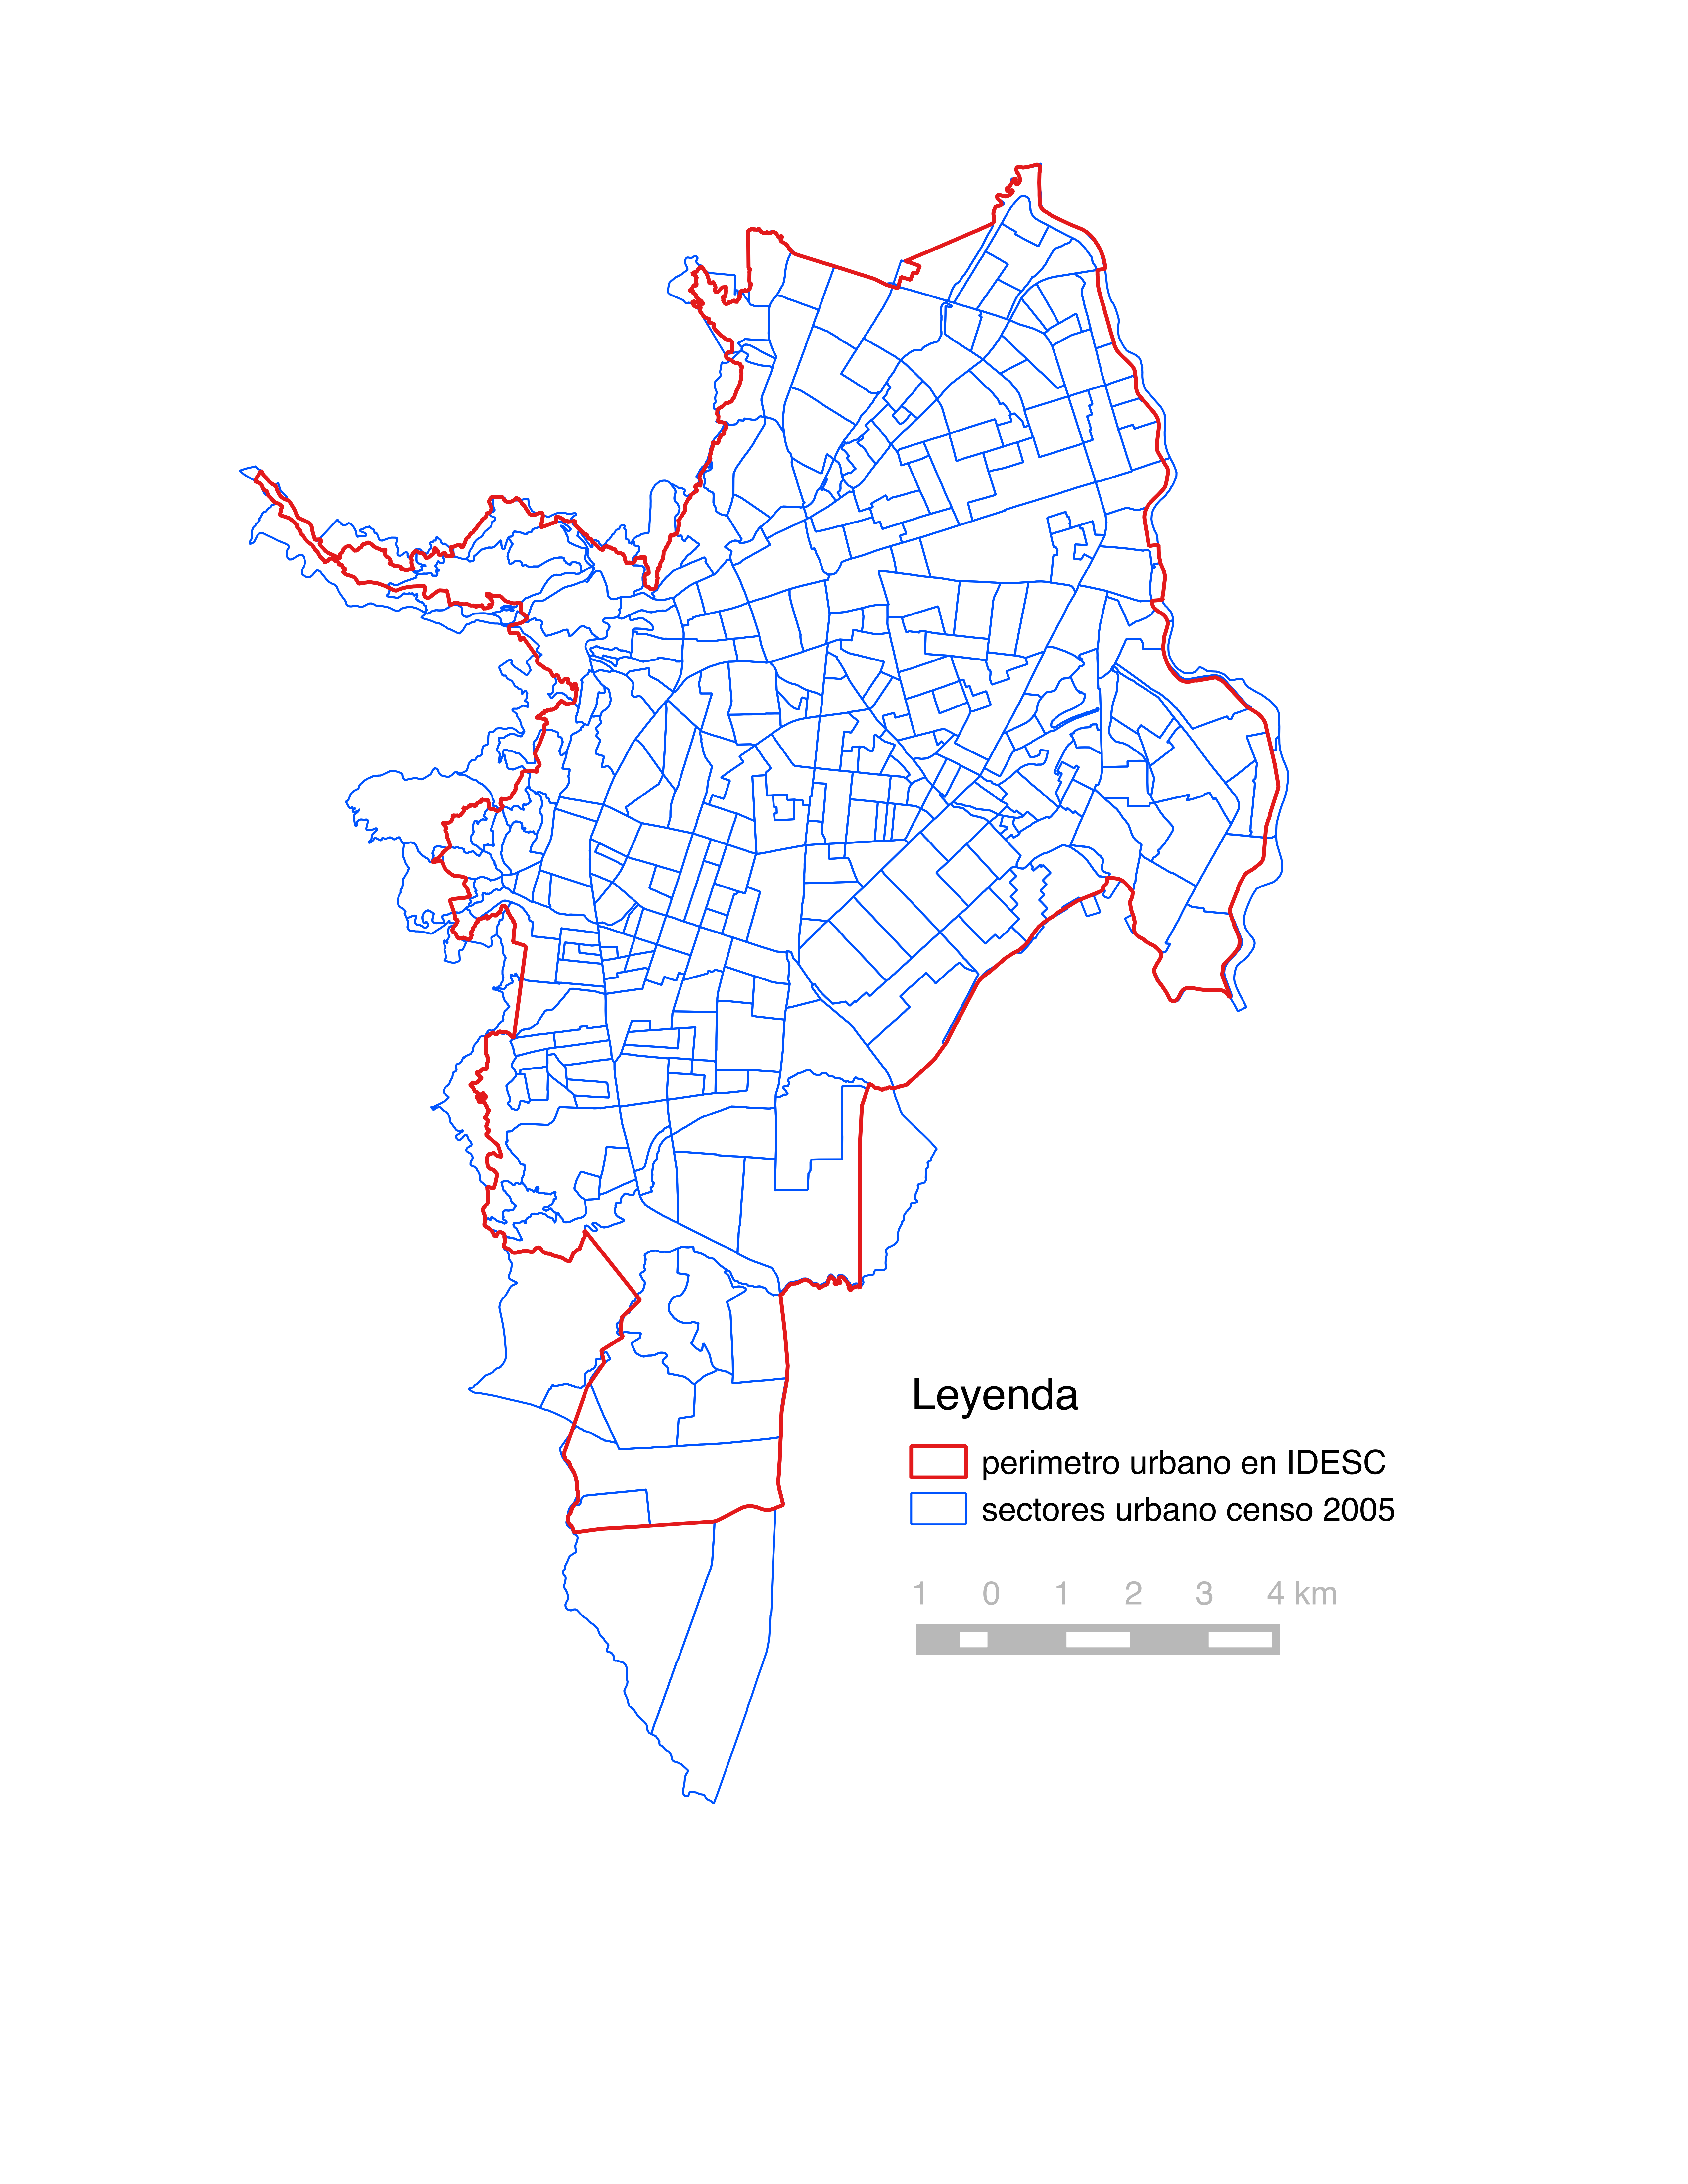
\includegraphics[width=1\linewidth]{images/sectoresurbanos_perimetro_idesc} \caption{División en barrios y sectores urbanos de Santiago de Cali}\label{fig:su-periurbano}
\end{figure}

\begin{longtable}[]{@{}rr@{}}
\caption{\label{tab:vars-vivienda} Variables sobre la las
viviendas}\tabularnewline
\toprule
\begin{minipage}[b]{0.09\columnwidth}\raggedleft\strut
variable\strut
\end{minipage} & \begin{minipage}[b]{0.38\columnwidth}\raggedleft\strut
\{valores\}{[}unidades{]}\strut
\end{minipage}\tabularnewline
\midrule
\endfirsthead
\toprule
\begin{minipage}[b]{0.09\columnwidth}\raggedleft\strut
variable\strut
\end{minipage} & \begin{minipage}[b]{0.38\columnwidth}\raggedleft\strut
\{valores\}{[}unidades{]}\strut
\end{minipage}\tabularnewline
\midrule
\endhead
\begin{minipage}[t]{0.09\columnwidth}\raggedleft\strut
tipo vivienda\strut
\end{minipage} & \begin{minipage}[t]{0.38\columnwidth}\raggedleft\strut
{[}viviendas{]} \{Casa,Casa indígena,Apartamento,Tipo cuarto,Otro tipo
de vivienda\}\strut
\end{minipage}\tabularnewline
\begin{minipage}[t]{0.09\columnwidth}\raggedleft\strut
uso vivienda\strut
\end{minipage} & \begin{minipage}[t]{0.38\columnwidth}\raggedleft\strut
{[}predio{]}\{Uso Vivienda.Uso Unidad Económica,Uso LEA\}\strut
\end{minipage}\tabularnewline
\begin{minipage}[t]{0.09\columnwidth}\raggedleft\strut
cantidad predios\strut
\end{minipage} & \begin{minipage}[t]{0.38\columnwidth}\raggedleft\strut
{[}predios{]}\strut
\end{minipage}\tabularnewline
\begin{minipage}[t]{0.09\columnwidth}\raggedleft\strut
cantidad viviendas\strut
\end{minipage} & \begin{minipage}[t]{0.38\columnwidth}\raggedleft\strut
{[}viviendas{]}\strut
\end{minipage}\tabularnewline
\bottomrule
\end{longtable}

Una de las apuestas del proyecto es incluir aspectos de los procesos de
desarrollo urbano a través de la idea de barrio: como unidad de
identidad cultural urbana y estructural, de características físicas y
habitacionales en las que confluyen las transformaciones que hacen los
habitantes y los diseños urbanos e intervenciones arquitectónicas de los
planeadores y constructores en la ciudad. La unidad espacial de análisis
sobre la cual se harán todas las agregaciones es el sector urbano (SU)
de la cartografía censal 2005.

\section{Métodos y técnicas}\label{metodos-y-tecnicas}

El análisis propuesto se compone de las siguientes actividades:

\begin{enumerate}
\def\labelenumi{\arabic{enumi}.}
\tightlist
\item
  Preparación de los datos: una tarea común pero crucial para el
  análisis de datos. La estandarización de las variables categóricas y
  la identificación de valores atípicos o inconsistentes es una base
  firme para la estimación de parámetros y obtener soluciones confiables
  y sensibles de interpretación. Los datos suelen estar usualmente en
  formatos para la lectura humana o con distinta estructura de las
  variables de los modelos. La preparación de los datos consume la mayor
  parte de los esfuerzos de las tareas de procesamiento de los datos.
  Los datos del censo arbóreo se encuentra en tablas bien conformadas lo
  que facilita su manipulación. Los datos de consulta del censo de
  población vienen en tablas independientes para cada unidad espacial
  seleccionada, con diferentes longitud de variables. A esto se suma el
  componente espacial, donde hay que prestar particular atención a los
  sistemas de coordenadas y usar coordenadas planas consistentes con las
  unidades de espacio.
\item
  Procesamiento y análisis estadístico: cálculo de indicadores de
  cobertura, acceso y variables socioeconómicas. Cálculo de estadísticos
  para probar normalidad, normalización de las variables e indicadores,
  cálculos de coeficientes de correlación Pearson y de Spearman entre
  todos los pares de variables.
\item
  Inspección visual de los datos: hacer uso de gráficas estadísticas,
  mapeos y mapas para evaluar y seleccionar los indicadores a usar en un
  modelo de regresión lineal.
\item
  Evaluar los residuos usando la prueba de correlación espacial de
  Moran'I usando al menos dos diseños de matriz W. Si la prueba muestra
  una correlación y un valor de significancia alta, se prueban modelos
  tipo SAR, SEM o SLX para comparar su desempeño.
\item
  Selección del modelo que mejor se ajusta usando métricas de error y de
  ajuste como R\textsuperscript{2} y el criterio de Akaike.
\end{enumerate}

\begin{figure}
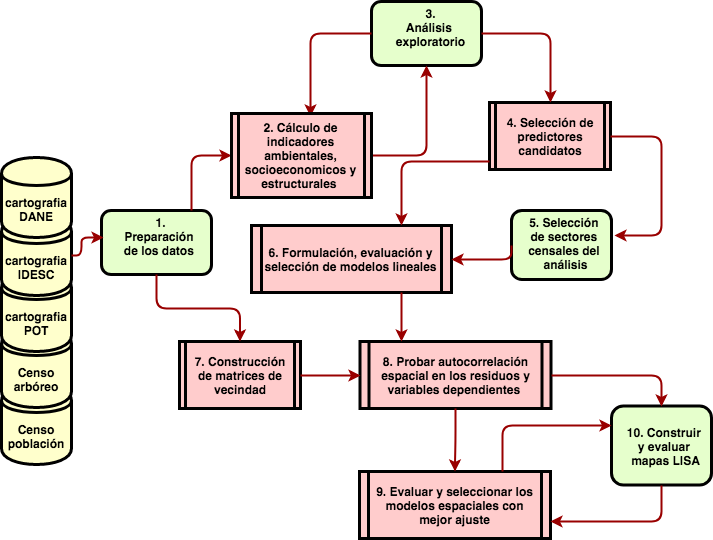
\includegraphics[width=1\linewidth]{images/flujograma} \caption{Diagrama de flujo de la metodología}\label{fig:flujograma}
\end{figure}

\subsection{Procesamiento de datos}\label{procesamiento-de-datos}

El procesamiento de los datos se realizó principalmente en
\citet{R-base}. Se usó \href{http://www.qgis.org/es/site/}{QGIS} para
conectarse a los servicios WFS del IDESC y previsualizar las capas de
información geográfica recolectada y la realización de algunos de los
mapas detallados.

El código que implementa los análisis está dividido en archivos para
facilitar su lectura, cada uno de los cuales se encargan de transformar
los datos de las fuentes y construir estructuras de datos necesarias
para realizar las regresiones, las gráficas y los análisis de tipo
estadístico y geoestadístico. Cada script implementa una fase de la
metodología y produce resultados intermedios que facilitan seguir y
reproducir dichas transformaciones sobre los datos de un dominio del
problema. El archivo de \texttt{funciones.R} agrupa funciones que
encapsulan funcionalidades recurrentes dentro del desarrollo del
análisis. El script de \texttt{geodata.R} opera sobre los fuentes de
datos geográficas necesarias para consolidar los índices de acceso a
espacios verdes (EV), los indicadores y variables de la estructura de
física de los sectores censales y unidades geográficas del análisis. El
script \texttt{arboles,R} consolida la información de cada uno de los
individuos del censo arbóreo agregandolos por sector censal. El scrript
\texttt{censopoblacion.R} consolida los datos del Censo de Población
2005. Los scripts \texttt{consolidarDatos.R} y
\texttt{analisis\_exploratorio.R} consolidan una única estructura con
todos los datos y produce una serie de gráficas y medidas de
correlación, que son base para la identificación de supuestos y
selección de las variables independientes para los análisis estadísticos
y las regresiones espaciales. Finalmente los script de
\texttt{analisis\_estadistico.R} y \texttt{analisis\_geoestadistico.R}
implementan las regresiones lineales y las regresiones espaciales
respectivamente, así como los test y tablas para la verificación de los
supuesto matemáticos y la verificación de la calidad de los resultados.
Todos estos están reunidos en un script que carga las librerías
necesarias y ejecuta secuencialmente cada de los scripts descritos.

Para usar la información geográfica de la cartografía censal y la
información del IDESC es necesario establecer un sistema de coordenadas
común, en unidades métricas, que facilite integrar la información y
produzca resultados consistentes. El sistema de coordenadas proyectadas
que vamos a usar es \citet{noauthor_magna-sirgas-cali_nodate}. Para
cargar y manipular los datos espaciales hacemos uso de las librerías
\texttt{rgdal} \citep{R-rgdal}, \texttt{rgeos} \citep{R-rgeos} y
\texttt{sp} \citep{R-sp}.

El código y los datos están disponibles en
\href{https://github.com/correajfc/R-CP2005-CA2015}{este repositorio de
GitHub}.

\subsection{Cálculo de métricas de acceso a servicios
ambientales}\label{calculo-de-metricas-de-acceso-a-servicios-ambientales}

\subsubsection{Indicadores de beneficios del arbolado
urbano}\label{indicadores-de-beneficios-del-arbolado-urbano}

Entre los distintos indicadores desarrollados para capturar la extensión
y distribución de los servicios ambientales la cobertura de copas ha
probado ser sensible y eficaz para cuantificar hasta qué punto los
árboles y bosques están proporcionando servicios críticos a los
residentes \citep{nowak_sustaining_2010}.

En este trabajo usaremos dos variantes de la cobertura de copa: el área
de copa en metros\textsuperscript{2} (\texttt{area\_copa}) y la
cobertura de copa como porcentaje del área pública total
(\texttt{cobertura\_copa.ap}), conformada por la vías y calles más el
área de espacio públicos) (ver figura \ref{fig:mapa-copa-dep}).

\begin{figure}
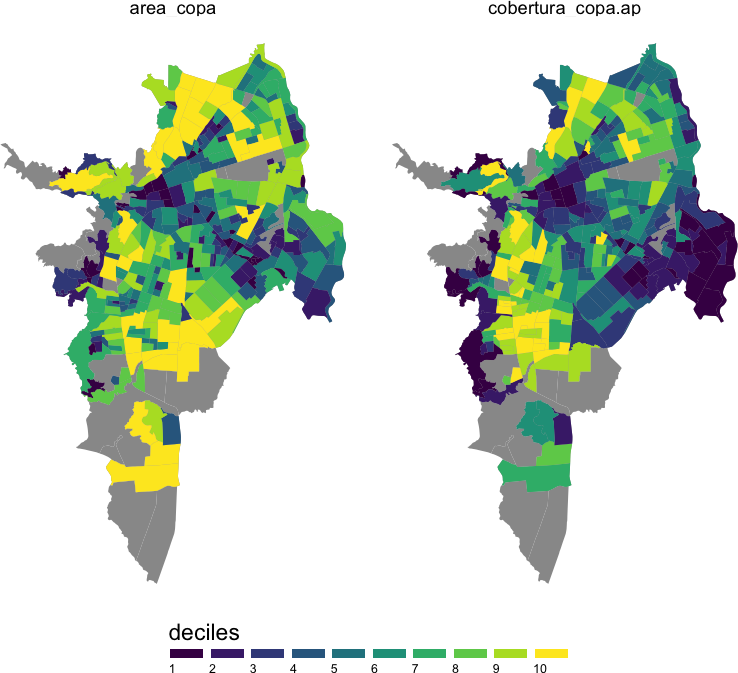
\includegraphics[width=1\linewidth]{tesis-unigis_files/figure-latex/mapa-copa-dep-1} \caption{Sectores urbanos de las variables dependientes sobre cobertura de copa}\label{fig:mapa-copa-dep}
\end{figure}

\subsubsection{Índices de acceso a espacios
verdes}\label{indices-de-acceso-a-espacios-verdes}

Para mejorar la lectura de esta sección se incluyen a continuación las
ecuaciones que definen los índices de acceso seleccionados con las
variantes definidas en este trabajo.

\textbf{índice contenedor porcentual} (area\_ep.porcentaje)

\begin{equation}
A^{C_p}_i =1/a_i\sum_j{s_j} \;  \; \forall  j \in I
\label{eq:n-cont}
\end{equation}

donde \(s_j\) es el área de cada espacio verde \(j\) que pertenece al
conjunto \(I\) de EV dentro del sector \(i\) y \(a_i\) es el área del
sector \(i\).

\textbf{razón área disponible distancia} (ia.areas.dist)

\begin{equation}
\bar{A}^{AD}_i= \frac{\sum_{\int R_b }{s_j}}{\sum_{\int R_b }{d_{ij}}}  \;  \; \forall  j \in I_{R_b} \; 
\label{eq:areas-dists}
\end{equation}

donde \(R_b\) es el radio de búsqueda, \(s_j\) es el área de cada
espacio verde \(j\), \(d_{ij}\) es la distancia del centriode del sector
\(i\) al espacio \(j\) que pertenecen al conjunto \(I_{R_b}\) de EVs en
el radio de búsqueda.

Este índice muestran un dimensión relacionada no con solo con el acceso
sino con la cantidad de espacio disponible en el radio de búsqueda
definido desde el centroide del sector censal. Para hacernos una idea
del radio de búsqueda seleccionado, el siguiente mapa muestra los radios
búsqueda y los espacios verdes.

\begin{figure}
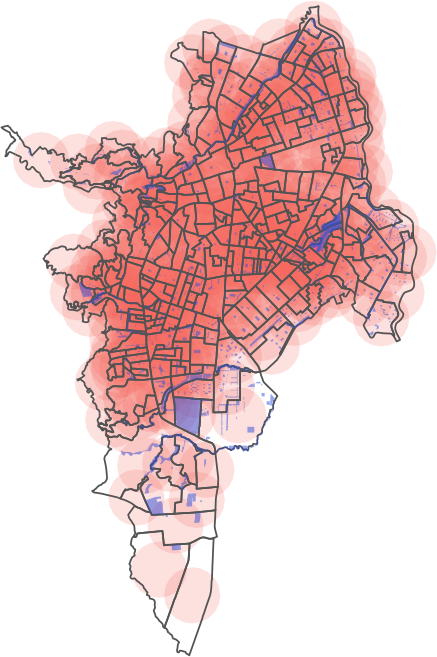
\includegraphics[width=1\linewidth]{tesis-unigis_files/figure-latex/mapa-rango1km-1} \caption{Espacio verdes y rango de 1 km desde centriodes de SU}\label{fig:mapa-rango1km}
\end{figure}

\subsection{Cálculo de métricas de sobre la
población}\label{calculo-de-metricas-de-sobre-la-poblacion}

\subsubsection{Características de la
población}\label{caracteristicas-de-la-poblacion}

La tabla \ref{tab:vars-poblacion} resumen las variables consideradas
inicialmente en este trabajo, sin embargo, algunas de ellas no contienen
suficiente variabilidad o el número de individuos es muy bajo en
comparación con el total de la población. En la tabla
\ref{tab:totales-poblacion} se observa el bajo número de personas que
pertenecen al pueblo Rom (gitanos), Palenqueros de San Basilio
(departamento de Bolívar) y de Raizales del Archipiélago de San Andrés,
Providencia y Santa Catalina (SAI), por lo que son descartados del
análisis al igual que la población indígena.

\begin{table}

\caption{\label{tab:totales-poblacion}Totales de población en la ciudad de Cali}
\centering
\begin{tabular}[t]{l|r}
\hline
Tipo & Cantidad\\
\hline
Población Total & 2027024\\
\hline
Población afrodescendiente, negros o mulatos & 530990\\
\hline
Población indígena & 9195\\
\hline
Población Rom & 690\\
\hline
Población Palenqueros & 1\\
\hline
Población raizales de SAI & 851\\
\hline
\end{tabular}
\end{table}

Las variables del censo de población seleccionadas para el análisis se
muestran en la figura \ref{fig:mapas-poblacion-deciles}

\begin{figure}
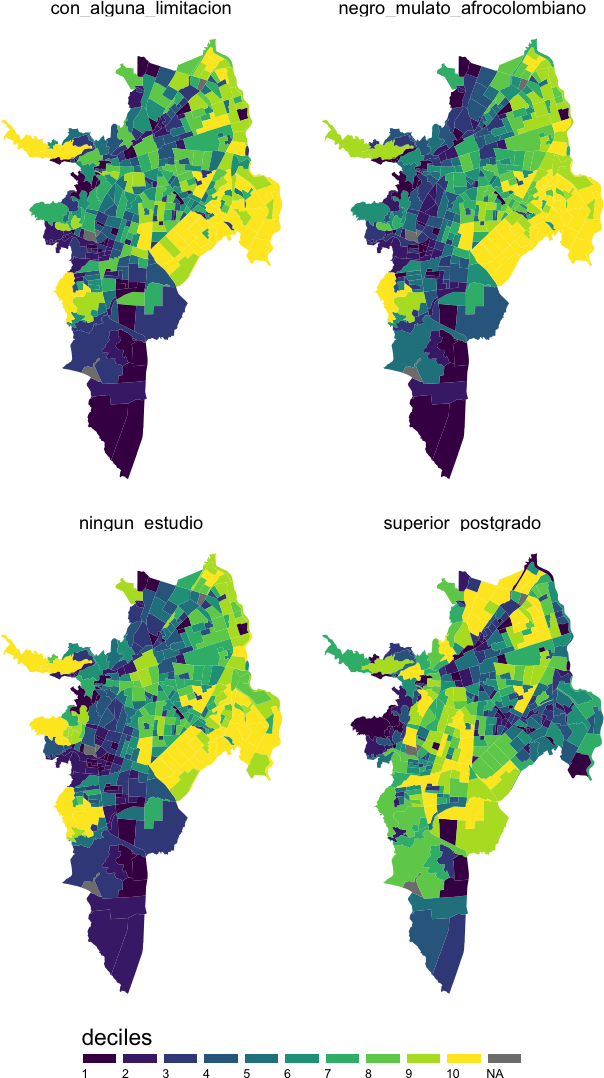
\includegraphics[width=1\linewidth]{tesis-unigis_files/figure-latex/mapas-poblacion-deciles-1} \caption{Mapas de las variables de población seleccionadas (en deciles)}\label{fig:mapas-poblacion-deciles}
\end{figure}

Además de las variables seleccionadas podemos calcular indicadores como
la densidad de población: dado que los árboles compiten por el espacio
con los seres humanos es de esperarse que a mayor cantidad de personas
haya menos lugar para los árboles. Podemos de nuevo calcular indicadores
porcentuales respecto de la población total de cada unidad geográfica
para facilitar la comparaciones y acentuar las diferencias entre los
diferente sectores (figura \ref{fig:mapas-poblacion-mod-deciles}).

\begin{figure}
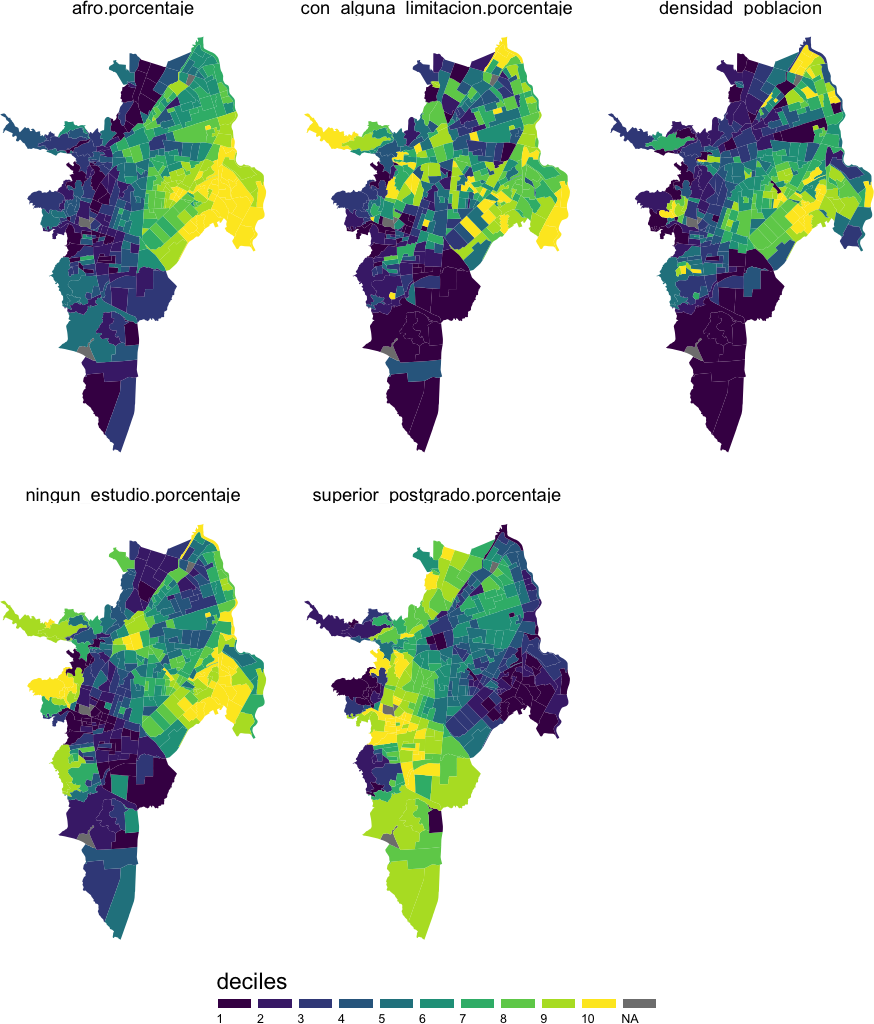
\includegraphics[width=1\linewidth]{tesis-unigis_files/figure-latex/mapas-poblacion-mod-deciles-1} \caption{Mapas de las variables de población seleccionadas como porcentajes (en deciles)}\label{fig:mapas-poblacion-mod-deciles}
\end{figure}

\subsubsection{Características de las
viviendas}\label{caracteristicas-de-las-viviendas}

Además de las rasgos étnicos, condiciones de estudio y limitaciones de
la población el censo de 2005 tiene disponibles datos sobre el tipo de
viviendas (casa, apartamento, tipo cuarto, casa indígena, otros), y el
uso habitacional, comercial y la cantidad de unidades especiales de
alojamiento L.E.A dado a los predios. La vocación comercial o
residencial de un barrio puede ser un factor en el desarrollo del
arbolado urbano o de las disposiciones urbanísticas de la ciudad en
relación a en EV, ya sea por las condiciones físicas como por la
intervención de sus habitantes. Estas variables pueden también
expresarse como porcentaje de la cantidad de predios de vivienda en el
caso de los tipos o como porcentaje de la cantidad de predios en el caso
del uso como unidad de vivienda, económica o L.E.A.

A continuación presentamos el resumen, los mapas por sector urbano
(figuras \ref{fig:mapas-usopredios-cont}.

\begin{figure}
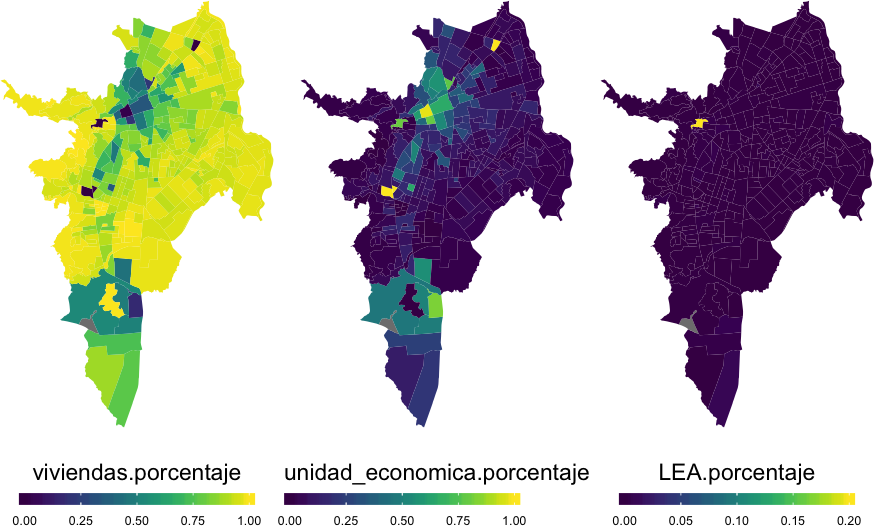
\includegraphics[width=1\linewidth]{tesis-unigis_files/figure-latex/mapas-usopredios-cont-1} \caption{Mapas de las variables sobre el tipo de uso de los predios como porcentaje de la cantidad de predios (escala contínua)}\label{fig:mapas-usopredios-cont}
\end{figure}

El uso de L.E.A tiene una distribución concentrada en uno pocos SU, por
lo que podemos descartarla para los análisis de regresión. Existe
también cierta complementariedad entre el uso de vivienda y los usos
económicos de los predios, porque seguramente, si existe una correlación
entre estas variables y la cobertura de copa o el acceso a espacios
verdes una de las dos puede bastar para incluir esta dimensión en los
modelos de regresión.

\subsection{Criterios y selección de sectores
censales}\label{criterios-y-seleccion-de-sectores-censales}

Antes de iniciar un análisis de regresión establecemos los criterios
para inclusión o no de ciertos datos dentro del conjunto de valores para
la regresión y cálculo de la correlación. Estos criterios se listan a
continuación:

\begin{itemize}
\tightlist
\item
  sectores sin personas
\item
  sectores sin viviendas
\item
  sectores área de espacio público mayor que el 60 \% del área del
  sector
\item
  sectores área de calle mayor que el 80 \% del área del sector
\item
  sectores área privada mayor que el 90 \% del área del sector
\end{itemize}

Además de estos criterios se excluyeron los sectores donde está la
Laguna el Pondaje, que cubre una porción muy importante del sector que
no se ve reflejado en las otras métricas, los sectores con una porción
mayor al 60\% por fuera del perímetro urbano o sin urbanización visible
en las imágenes satelitales. Así los sectores excluidos del análisis se
muestran en los mapas \ref{fig:mapa-excluidos}.

\begin{figure}
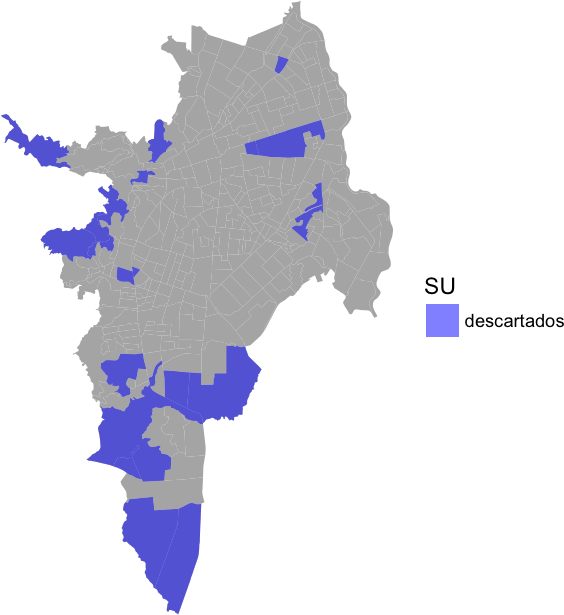
\includegraphics[width=1\linewidth]{tesis-unigis_files/figure-latex/mapa-excluidos-1} \caption{Mapa de los sectores excluidos}\label{fig:mapa-excluidos}
\end{figure}

\subsection{Selección de variables dependientes y regresiones
lineales}\label{seleccion-de-variables-dependientes-y-regresiones-lineales}

Las variables a incluir en los modelos lineales deben cumplir una serie
de condiciones para ser elegidas como candidatas:

\begin{itemize}
\tightlist
\item
  \emph{Mostrar una correlación fuerte} (típicamente mayor a 0.6 se
  considera una asociación fuerte).
\item
  \emph{Las variables independientes o predictoras no deben estar
  fuertemente correlacionadas entre ellas}.
\item
  \emph{Las observaciones deben ser independientes}. En nuestro caso
  significa que no debe existir relación espacial o temporal entre los
  diferentes sectores. Justamente esto se pondrá a prueba con los test
  estadísticos y los graficos de diagnostico sobre la distribución de
  los residuos de la regresión: se espera que dicha dependencia esté
  motivada por la vecindad de los sectores.
\item
  \emph{Las variables dependientes e independientes deben tener una
  distribución normal}. Esta condición no suele ser estricta, pues lo
  importante es que al calcular los coeficientes de la regresión
  obtengamos una distribución normal de los residuos (sin ningún patrón,
  ruido). De no ser así, es posible que las variables no sean
  independientes o que exista información significativa en los residuos,
  por ejemplo, porque existe autocorrelación espacial en la variable
  dependiente y entonces la regresión lineal no obtiene resultados
  confiables para los coeficientes.
\end{itemize}

La modelación inicia con el análisis con las variables sobre la
población, que son las de mayor interés en un estudio dado su enfoque en
la justicia ambiental, para luego incorporar las variables de los
dominios relacionados con el uso de los predios, los tipos de viviendas
y la existencia de espacios verdes como parques, bulevares, escenarios
deportivos o plazas, alojan una cantidad considerable de los individuos
arbóreos de la ciudad.

Para garantizar que las variables no están correlacionadas entre sí,
usaremos los coeficientes de correlación de Pearson, usado para detectar
relaciones lineales, usualmente en variables con distribución normal, y
el coeficiente de Spearman para detectar relaciones en variables con
otras distribuciones o que exhiben relaciones no lineales. Para tener
una idea más amplia sobre esa relación que expresan los coeficiente de
correlación se incluyen gráficas de dispersión entre las variables
independientes, y entre dependientes.

Para seleccionar las variables que mejor predicen la cobertura de copa
aplicamos un procedimiento análogo al realizado con las variables
dependientes entre sí. Con base en los coeficientes de correlación de
Pearson y Spearman entre las variables dependientes e independientes, y
teniendo en cuenta las restricciones de colinealidad entre las variables
dependientes, seleccionamos las variables a usar en el modelo lineal.

Antes ajustar los modelos suele ser común en los modelos de regresión
ajustar la distribución de las variables dependientes (y a veces las
independientes) por motivos teóricos usando transformaciones
logarítmicas o de raíz cuadra para eliminar no linealidades entre las
variables dependientes y las independientes, y reducir posibles
fenómenos de heterocedasticidad debido a estas no-linealidades.

Dividir o multiplicar por alguna constante no tiene ningún efecto en la
calidad de las estimaciones , pero sí sobre los coeficientes de la
regresión. Esto suele ser sensible a la hora de interpretar los cambios
marginales de cada una de las variables independientes y su efecto sobre
la variable dependiente. Sin embargo, lo que interesa para este estudio
no es la interpretación de esos cambio sino la importancia relativa de
cada variable y comparar los cambios de los coeficientes de regresión
para el ajuste de cada modelo y/o las mejoras que pueda operar un
modelos autorregresivo en caso de encontrase autocorrelación en los
residuos de la regresión lineal. Por esta razón, normalizar los valores
puede ser una ventaja pues mantiene los coeficiente mejor acotados. La
normalización se aplica posterior a las transformaciones propuestas y se
realiza dividiendo por el máximo valor de los datos de cada variable
para mantener valores en el intervalo {[}0,1{]}, dado que los valores
son todos iguales o mayores que 0.

Al aplicar test para verificar que las condiciones de un buen ajuste (no
hay sesgos en el estimador o una mala especificación del modelo) de un
modelo lineal se cumplen:

\begin{itemize}
\tightlist
\item
  La media de los residuos es 0 o muy cercana.
\item
  La distribución de los residuos es normal.
\item
  Los residuos muestran homocedasticidad (la varianza es constante)
\end{itemize}

Para verificar la normalidad de los residuos se hace uso del test de
Shapiro--Wilk \citep[ ]{shapiro1965analysis} y para la verificar si
existe homocedasticidad el test de Breusch--Pagan
\citep{breusch1979simple}.

\subsection{Análisis geoestadísticos}\label{geostat}

Para los análisis geoestadísticos introducimos los modelos
autoregresivos para obtener mejoras en la estimación de los coeficientes
y en el ajuste de los modelo si existe algún tipo de autocorrelación
espacial en los residuos. Existe una variedad de estos modelos que
capturan diferentes tipos de efectos: modelo autoregresivo SAR que
capturan efectos de la variable dependiente, ecuación \eqref{eq:sar} ,
sobre las variables las independientes ( spatial lag o retardo espacial
en \(X\) SLX, ecuación \eqref{eq:slx}, en el error (modelo espacial del
error SEM, ecuación \eqref{eq:sem} o usando una combinación del modelo de
error y autoregresivo (modelo espacial de Durbin SD,ecuación
\eqref{eq:sd}. Todas estas aproximaciones introducen una matriz de
\(W_{n \times n}\), donde \(n\) es el número de sitios, que captura la
influencia de las variables en relación con su proximidad. Esta matriz
\(W\) es una estructura que restringe la influencia a priori en el
modelo. Para observar el efecto que tiene esta matriz sobre los
resultados del modelo usaremos 2 matrices distintas, y veremos su
impacto en la estimación.

Para los análisis espaciales usaremos la librería \texttt{spdep}
\citep{R-spdep}

\subsubsection{Matrices de vecindad}\label{matrices-de-vecindad}

La matriz \(W\) representa la topología de vecindad entre los sectores
censales. Existen la literatura diferentes tipos de vecindad:
\emph{rook}, \emph{bishop} y \emph{queen} son las más referenciadas.
Esta vecindad está representada en la matriz con 1 cuando existe
vecindad y 0 cuando no. Otra forma de cuantificar la interacción de esa
vecindad es usando una matriz de inversos de la distancia entre los
centroides de los sectores censales, con el fin de atenuar la
interacción entre sectores muy alejados y tener una variable continua
que representa esa influencia. En la figura \ref{fig:w-su-todos} se
muestra la matriz \(W\) defina para vecinos que comparten un lado del
polígono (vecindad \emph{rook}) para todos los sectores de la ciudad de
Cali.

\begin{figure}
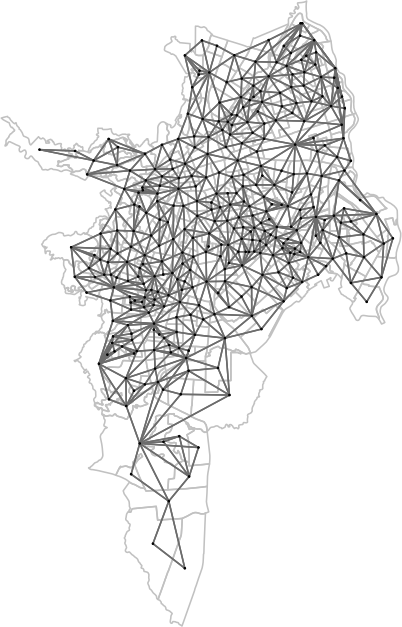
\includegraphics[width=1\linewidth]{tesis-unigis_files/figure-latex/w-su-todos-1} \caption{Grafo de vecindad entre todos los SU de la ciudad de Cali}\label{fig:w-su-todos}
\end{figure}

Sin embargo, la regresiones se realizan sobre un subconjunto de los
datos, y por tanto la estructura de esta matriz debe tener esto en
cuenta, o mejor, no tener en cuenta la influencia de estos sectores
excluidos. Se calculó cada par de matrices de vecindad propuestas con
base en el subconjunto de datos usados en los espacios verdes y para
sectores del analsis del arbolado urbanos. Así la matriz de vecindad
para los SU usados para la estimación de los coeficientes de las
regresiones lineales se ve en la figura \ref{fig:w-su-reg}.

\begin{figure}
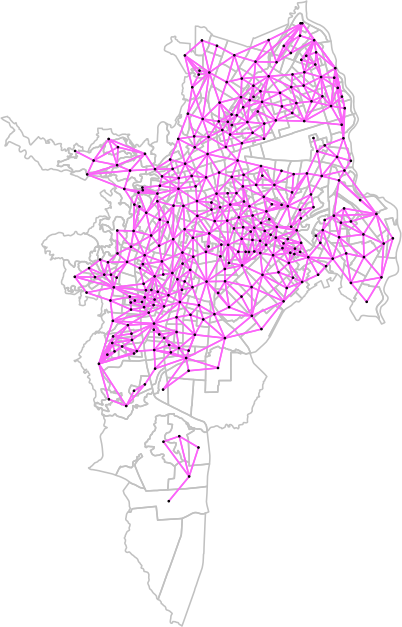
\includegraphics[width=1\linewidth]{tesis-unigis_files/figure-latex/w-su-reg-1} \caption{Grafo de vecindad entre los SU seleccionados para el análisis del AU}\label{fig:w-su-reg}
\end{figure}

La matriz \(W_d\) impone un estructura de interacciones que puede
relacionar sectores en una zona que no necesariamente comparten ningún
lado o esquina pero que están cercanos, mientras que \(W_q\) se
restringe a condiciones de vecindad sólo entre sectores contiguos. En
esa medida puede existir juego para dar interpretación teórica al
fenómeno de derrame o influencia que ejercen sobre el ajuste de los
modelos. Un ejemplo puede ser que la dependencia espacial de las
cobertura de árboles que expresa \(W_d\) es una característica en una
zona no limitada por las divisiones del territorio con base en los
desarrollos urbanísticos (barrios) sino que se ajustan más a fenómenos
de dispersión continuos con base en el alcance escogido. Así, la \(W_q\)
puede interpretarse como una forma de dar relevancia a la continuidad
entre barrios y su importancia como unidad de desarrollo urbano en las
variaciones de la variable a predecir.

\subsubsection{Autocorrelación espacial}\label{autocorrelacion-espacial}

Para indagar sobre la información o patrones espaciales de los residuos
de los modelos de regresión usaramos el índice de Moran I. El índice de
Moran I es el coeficiente de correlación para la relación entre una
variable y sus valores circundantes. Si encontramos una correlación
espacial significativa en los residuos, esto sugiere que agregando esa
estructura en el modelo podremos obtener una estimación más eficiente de
los coeficientes, y en consecuencia un mejor entendimiento de la
relación entre esas variables. Hay que recordar que en este ejercicio no
estamos queriendo entender una población por una muestra, estamos
calculando estos coeficientes sobre el total de la población, y por
tanto los coeficientes pueden interpretarse como la fuerza de esa
relación. La confianza en esa estimación depende de que los residuos
obtenidos sean tenga un valor medio de 0, y que no puedan distinguirse
del ruido. La ecuación \eqref{eq:moranI} define matemáticamente el índice:

\begin{equation}
 I=\frac {N}{\sum _{i}\sum _{j}w_{ij}} \frac {\sum _{i}\sum _{j}w_{ij}(X_{i}-{\bar {X}})(X_{j}-{\bar {X}})}{\sum _{i}(X_{i}- \bar{X})^{2}}
\label{eq:moranI}
\end{equation}

donde \(N\) es el número de unidades espaciales indexados por \(i\) y
\(j\); \(X\) es la variable de interés; \(\bar {X}\) es la media de
\(X\); y \(w_{ij}\) es un elemento de una matriz de pesos espaciales
\(W\). Un valor de 0 de Moran'I indica un patrón espacial aleatorio. Si
existe autocorrelación los valores son positivos y el máximo es 1. Si
los valores son negativos decimos que existe dispersión, siendo -1 el
mínimo valor posible representando la dispersión perfecta.

El gráfico de Moran es una forma de observar el valor de la pendiente
(el índice de autocorrelación) graficando los valores retardados
(spatial lag: es como dijimos previamente el valor medio de los valores
vecinos) de la variable en cuestión en el eje \(y\) y la variable en el
\(x\). El valor \textbf{\(p\)} del test estadístico nos dice qué tan
seguros estamos que esa pendiente no es plana, por lo que se espera que
sean menores que el valor límite de significancia \(\alpha = 0.05\)

\begin{quote}
El hecho de que de la Morán I es una suma de productos cruzados
individuales es explotado por los ``indicadores locales de asociación
espacial'' (LISA) para evaluar la agrupación de las unidades
individuales mediante el cálculo de la I de Moran local para cada unidad
espacial y la evaluación de la significación estadística para cada I.
\citep{wikilisa}
\end{quote}

Estos mapas acompaña el resultado numérico y el gráfico de Moran
representan el valor z-normalizado del LISA, el valor \(p\) y el mapa de
clusters. En este último mapa las regiones resaltadas en rojo tienen
valores altos de la variable y tienen vecinos con valores altos también
(\emph{high-high}). El área azul es \emph{low-low} los grupos presentan
valores bajos al igual que sus vecinos. Mientras que las regiones azul
pálido son \emph{low-high} y las áreas rosadas son \emph{high-low}
muestran correlación negativa, es decir valores muy diferentes a los de
sus vecinos. Las regiones fuertemente coloreadas son aquellas que
contribuyen significativamente a un resultado positivo de
autocorrelación espacial global, mientras que los colores más claros
contribuyen significativamente a un resultado de autocorrelación
negativo.

\subsubsection{Ajuste de modelos
espaciales}\label{ajuste-de-modelos-espaciales}

Mejorar la especificación de los modelos lineales incluyendo términos de
retardo espacial en la variable dependiente (SAR \eqref{eq:sar}) se hace
para obtener una adecuada estimación de los coeficientes de las otras
covariables en el modelo. Si optamos por un modelo de error espacial
(SEM \eqref{eq:sem}) implica que no es necesario plantear efectos
distintivos de la variable dependiente rezagada, y que es posible que
ese efecto sea por otras variables no tenidas en cuenta: el agrupamiento
espacial observado en la variable dependiente se explica simplemente por
el patrón geográfico de variables independientes medidas y no medidas.
El modelo SAR, en cambio, incorpora la influencia de variables
independientes no medidas, pero también estipula un efecto adicional de
valores de atributos vecinos, es decir, la variable dependiente
rezagada. Si incluimos el retardo sólo de las variables independientes
(SLX \eqref{eq:slx}) esperamos que los cambios en las dimensiones
expresadas con las predictores produce un efecto de derrame o influencia
en los sectores vecinos.

¿Qué significa decir que la cantidad de cobertura de copa está
relacionada con la de los sectores vecinos?¿Son los procesos de
reproducción del arbolado urbano un fenómeno independiente de las
intervenciones de sus habitantes y de los urbanizadores?¿Los habitantes
que ven árboles en las cuadras o barrios aledaños deciden sembrar
árboles en su vecindario?¿Existen similitudes en las condiciones
estructurales de los barrios en ciertas zonas de la ciudad que prefieren
las personas con mejores condiciones sociales( tener estudios superiores
p.e)?¿Qué tipo de pérdidas en la cobertura de copa están motivadas por
la densificación de un sector? ¿Cómo afectan los cambios en los tipos de
oferta habitacional en un sector la cobertura de copa de los sectores
vecinos? (las viviendas tipo cuarto suelen ofrecerse en pensiones y ser
más económicas que las casas o apartamentos).

La pregunta a hacerse es cómo saber cuál de los diferentes modelos
espaciales es el que mejor representa el fenómeno que estamos modelando
y si los datos respaldan nuestras convicciones teóricas. Si el modelo de
retraso espacial que especifique es realmente el correcto, entonces
ninguna dependencia espacial debe permanecer en los residuos, y podremos
elaborar sobre el tipo de procesos que pueden verse representados.

Una alternativa metodológica es probar los 4 tipos de modelos con la
matriz \(W\) que resultó capturar mejor la asociación espacial en los
datos y comparar sus resultados.

\chapter{Resultados}\label{results}

\section{Modelando la cobertura de
copa}\label{modelando-la-cobertura-de-copa}

\subsection{Correlaciones y gráficos de dispersión
bivariados}\label{correlaciones-y-graficos-de-dispersion-bivariados}

En la figura \ref{fig:bivar-poblacion-abs} se explora las relaciones
entre las variables de población en las unidades originales de los datos
(número de personas); la matriz triangular superior muestra los
coeficientes de correlación de Pearson, la diagonal contiene el
histogram de frecuencias de la variable y la matriz triangular inferior
muestra un gráfico de dispersión y la línea de tendencia usando un
modelo lineal entre cada par de variables. Es notoria la alta
correlación entre tener ningún estudio y tener alguna limitación física
(0.88); pertenecer a una comunidad afrodescendiente y carecer de
estudios (0.92) o ser afrodescendiente y tener alguna limitación (0.88).
Esto representa una suma de condiciones desfavorables relacionadas entre
sí, que desde el punta del vista del modelo sólo podrán ser
representadas por una de las variables, la que mejor se relacione con la
cobertura de copa y evitar así colinealidad entre los predictores.

\begin{figure}
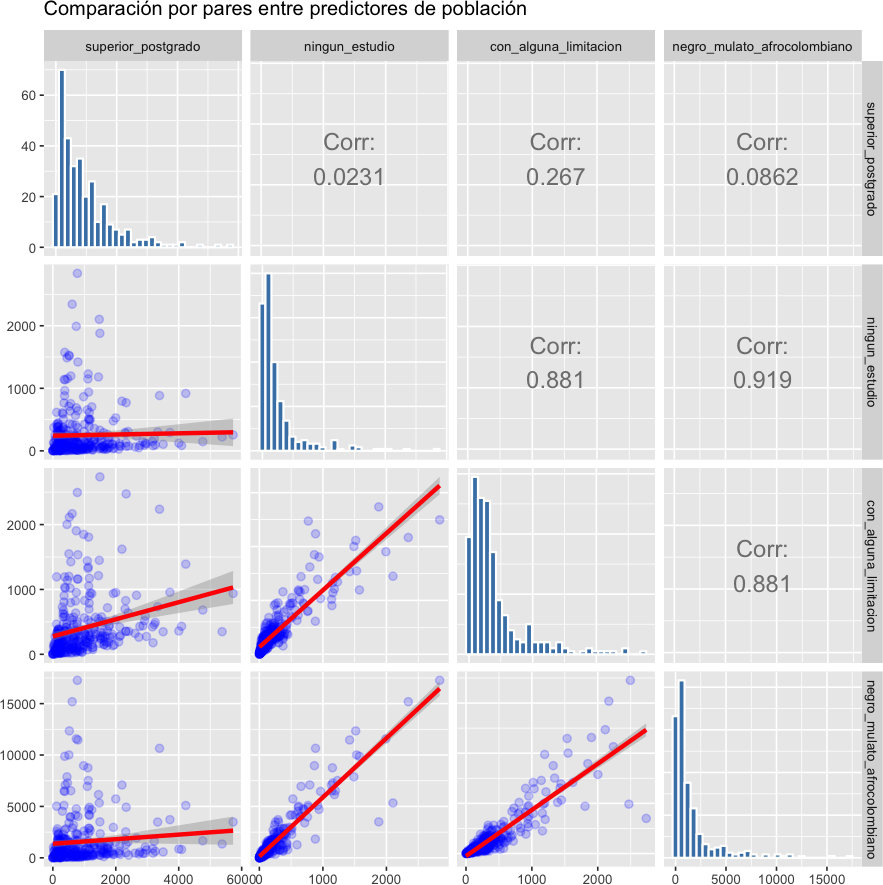
\includegraphics[width=1\linewidth]{tesis-unigis_files/figure-latex/bivar-poblacion-abs-1} \caption{Comparación por pares entre predictores de población}\label{fig:bivar-poblacion-abs}
\end{figure}

Cuando realizamos la misma comparación entre las variables porcentuales
(más la densidad poblacional) se observan patrones similares(ver figura
\ref{fig:bivar-poblacion-mod}): existe una alta correlación negativa
entre el porcentaje de población afro de un sector y la tenencia de
estudios superiores (-0.71), una fuerte asociación positiva entre el
porcentaje de personas afro de un sector y el porcentaje de personas que
carecen de estudios (0.68). También hay una fuerte relación inversa
entre el porcentaje de personas de un sector sin estudios y el
porcentaje de ellos que tiene estudios superiores (-0.8). Estas
variables evitaremos usarlas como predictores en una misma formulación
para no sesgar la estimación con problemas de colinealidad. Existe
también una asociación, no tan fuerte pero importante, entre la densidad
de población y sectores con mayor porcentaje de personas afro (0.47) y
una asociación negativa entre la densidad de población y el porcentaje
de personas con estudios superiores (-0.51). Estos resultados hablan de
una concentración de condiciones desfavorables para la población,
posiblemente acompañado de una segregación racial alta.

\begin{figure}
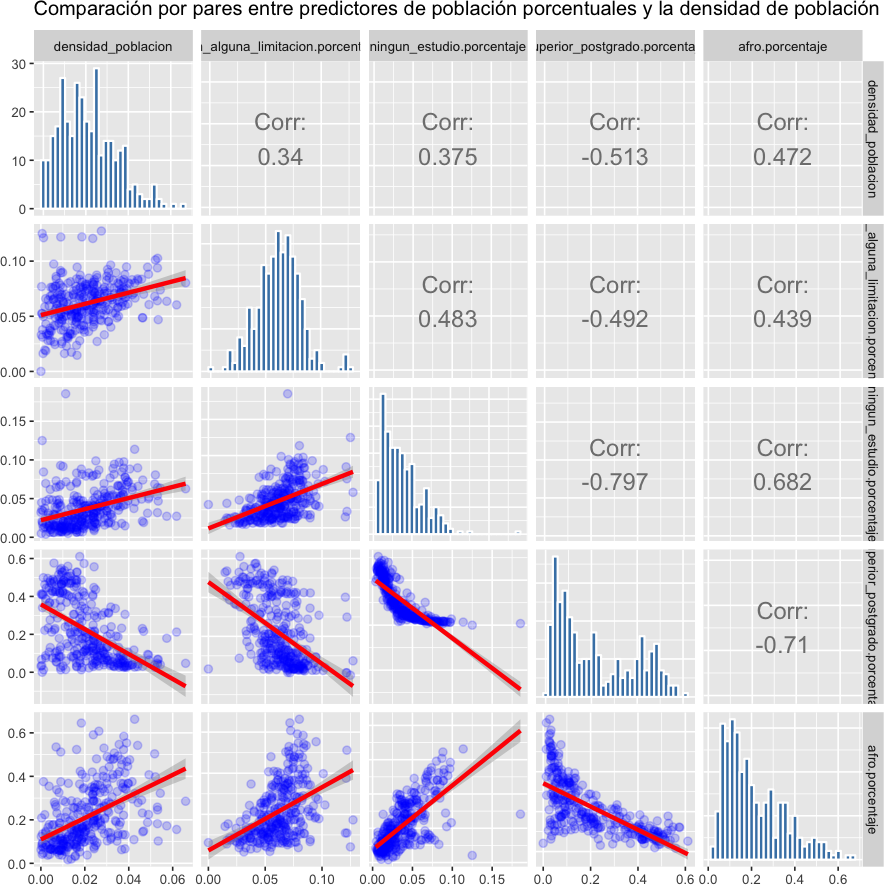
\includegraphics[width=1\linewidth]{tesis-unigis_files/figure-latex/bivar-poblacion-mod-1} \caption{Comparación por pares entre predictores de población porcentuales}\label{fig:bivar-poblacion-mod}
\end{figure}

Ya que hemos explorado visualmente la dispersión entre los datos crudos,
podemos usar una forma resumida, como los gráficos de azulejos o de
matriz para consultar la intensidad de estas relaciones (figura
\ref{fig:tile-poblacion-pearson} sintetiza las relaciones lineales entre
las variables dependientes, mientras que la figura
\ref{fig:tile-poblacion-pearson} lo hace para las no lineales)

\begin{figure}
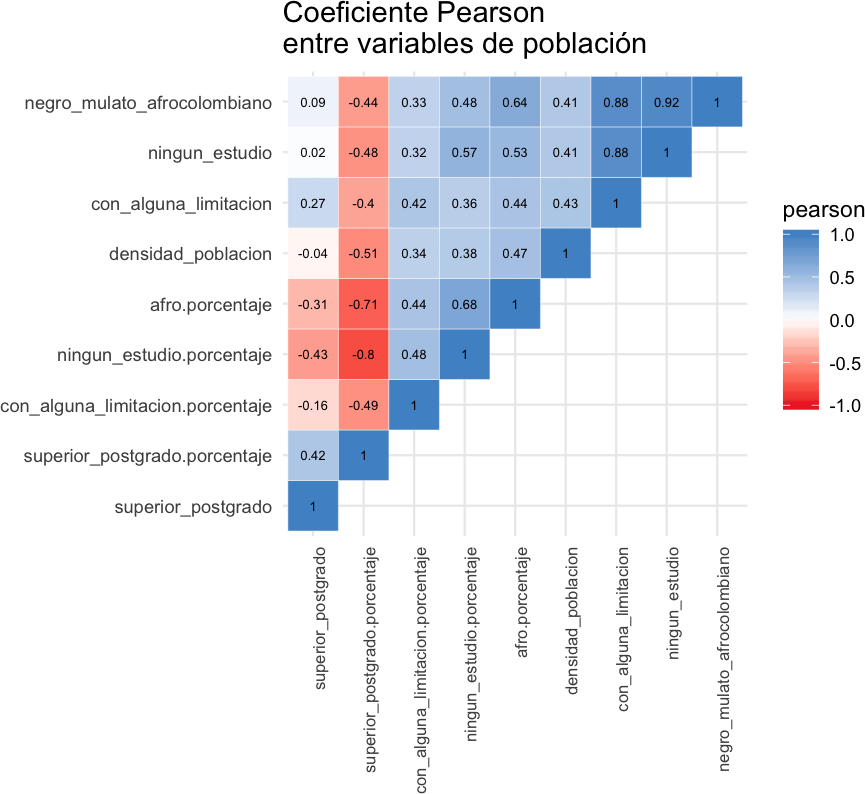
\includegraphics[width=1\linewidth]{tesis-unigis_files/figure-latex/tile-poblacion-pearson-1} \caption{Coeficiente Pearson entre variables de población}\label{fig:tile-poblacion-pearson}
\end{figure}

\begin{figure}
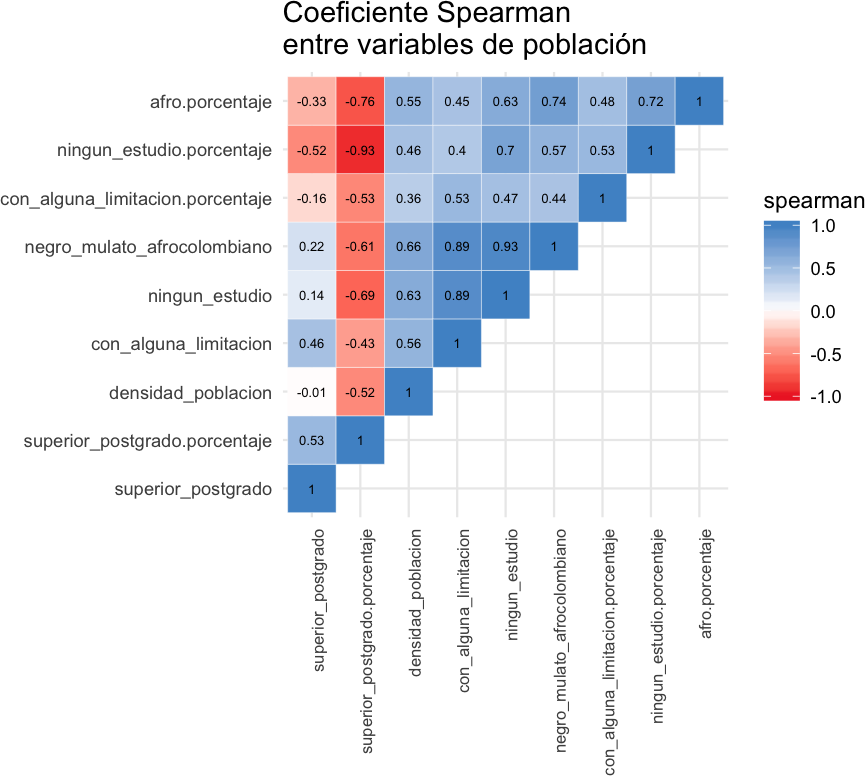
\includegraphics[width=1\linewidth]{tesis-unigis_files/figure-latex/tile-poblacion-spearman-1} \caption{Coeficiente Spearman entre varibles de población}\label{fig:tile-poblacion-spearman}
\end{figure}

Para seleccionar las variables que mejor predicen la cobertura de copa
aplicamos un procedimiento análogo al realizado con las variables
dependientes entre sí. Con base en los coeficientes de correlación de
Pearson (figura \ref{fig:tile-copa-poblacion-pearson}) y Spearman
(figura \ref{fig:tile-copa-poblacion-spearman}) entre las variables
dependientes e independientes, y teniendo en cuenta las restricciones de
colinealidad entre las variables dependientes, seleccionamos las
variables a usar en el modelo lineal.

Así pues, para el área de copa (\texttt{area\_copa}) los predictores
seleccionados
son\texttt{superior\_postgrado,\ densidad\_poblacion,\ con\_alguna\_limitacion.porcentaje,\ afro.porcentaje}
y para la cobertura de copa en área pública
(\texttt{cobertura\_copa.ap}) los predictores seleccionados
son\texttt{superior\_postgrado.porcentaje,\ densidad\_poblacion,\ con\_alguna\_limitacion.porcentaje,\ afro.porcentaje}

\begin{figure}
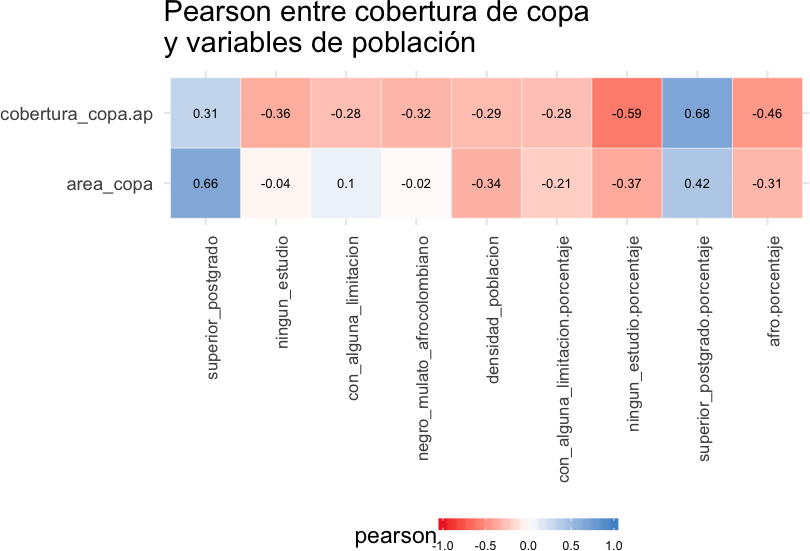
\includegraphics[width=1\linewidth]{tesis-unigis_files/figure-latex/tile-copa-poblacion-pearson-1} \caption{Coeficiente Pearson entre cobertura de copa
 y variables de población}\label{fig:tile-copa-poblacion-pearson}
\end{figure}

\begin{figure}
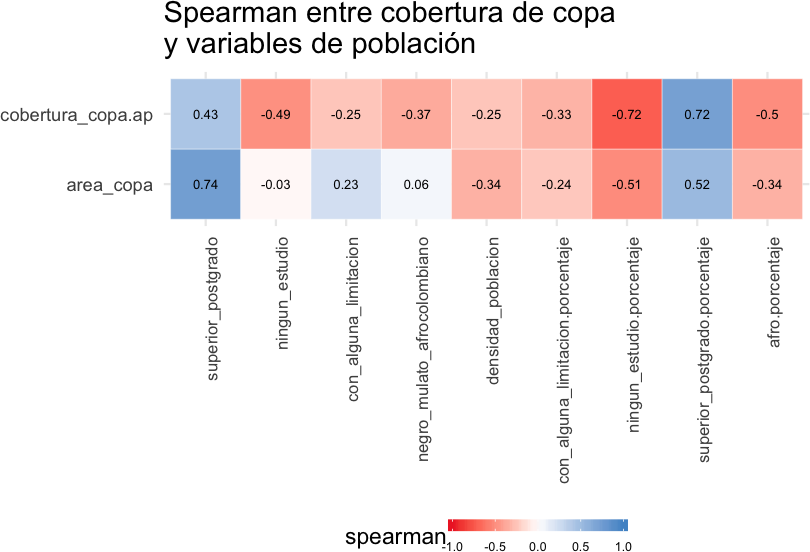
\includegraphics[width=1\linewidth]{tesis-unigis_files/figure-latex/tile-copa-poblacion-spearman-1} \caption{Coeficiente Spearman entre cobertura de copa
 y variables de población}\label{fig:tile-copa-poblacion-spearman}
\end{figure}

Para la selección de variables sobre uso de los predios, los tipos de
vivienda, áreas de espacio público y manzanas agregadas por sector
urbano aplicamos el mismo proceso realizado para la selección de las
variables de población usando como criterio la inclusión de variables
con coeficientes de correlación que muestran una asociación fuerte con
las variables de cobertura y área de copa.

Las figuras \ref{fig:tile-prediosev-pearson} y
\ref{fig:tile-prediosev-spearman} se ven los coeficientes de Pearson y
Spearman, respectivamente, entre las variables sobre el uso los predios,
tipo de viviendas y área (y porcentaje) de espacios verdes en cada
sector urbano. Como se observa, existe una fuerte (perfecta) asociación
negativa entre el porcentaje de casas y apartamentos, lo que obliga a
solo escoger una de las dos en caso de haber una fuerte relación entre
alguna de ellas con las variables de cobertura de copa. También hay una
fuerte asociación positiva entre el área de espacios verdes y el
porcentaje de área de espacio verdes en un sector urbano. Como
mencionamos antes solo incluiremos una de las dos en caso de que ambas
resulten fuertemente asociadas con las variables dependientes.

\begin{figure}
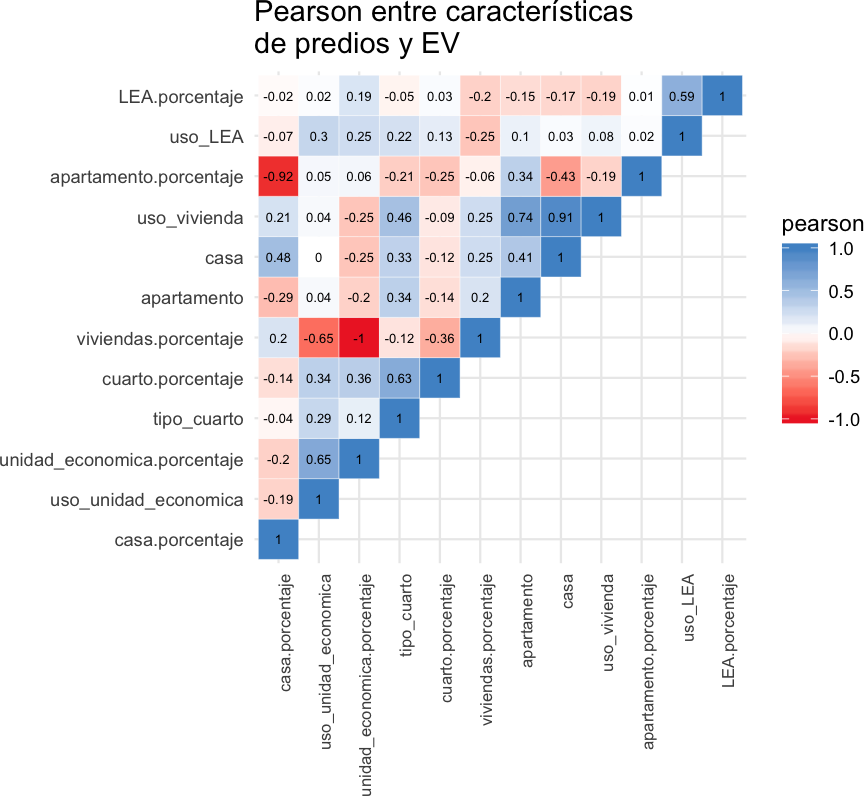
\includegraphics[width=1\linewidth]{tesis-unigis_files/figure-latex/tile-prediosev-pearson-1} \caption{Coeficiente Pearson entre variables de uso de los predios
 y espacios verdes en los sectores urbanos}\label{fig:tile-prediosev-pearson}
\end{figure}

\begin{figure}
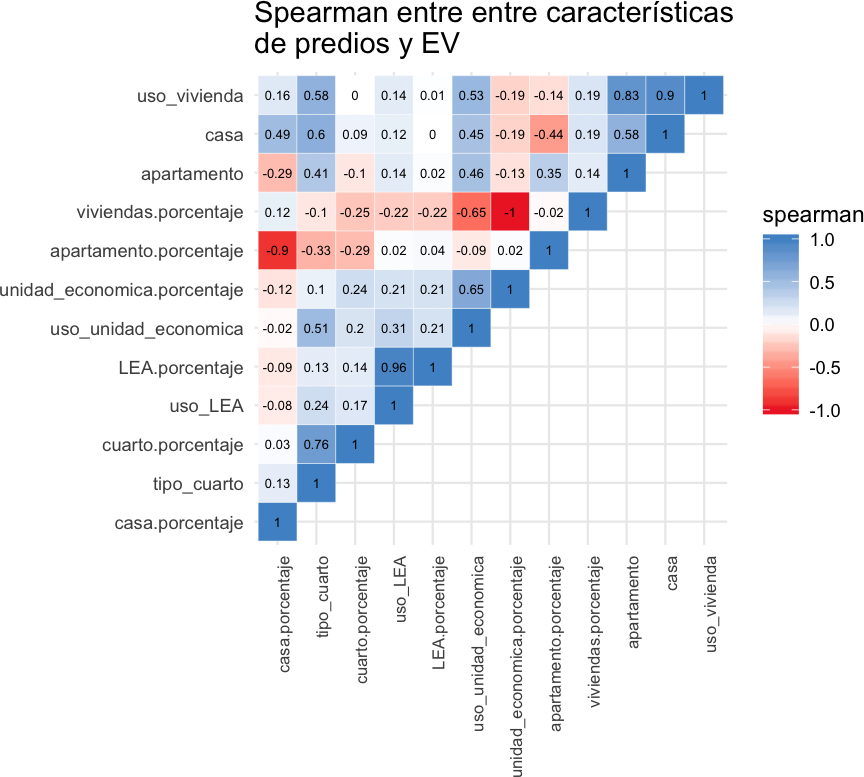
\includegraphics[width=1\linewidth]{tesis-unigis_files/figure-latex/tile-prediosev-spearman-1} \caption{Coeficiente Pearson entre variables de uso de los predios
 y espacios verdes en los sectores urbanos}\label{fig:tile-prediosev-spearman}
\end{figure}

Las figuras \ref{fig:tile-copa-prediosev-pearson} y
\ref{fig:tile-copa-prediosev-spearman} muestran la correlación entre las
potenciales nuevas variables a incluir en el modelo y las variables
dependientes de cobertura y área de copa. Para el área de copa se
seleccionan el área de espacios verdes (\texttt{area\_ep}) y el
porcentaje de viviendas tipo cuarto (\texttt{cuarto.porcentaje}). Para
el modelo de porcentaje de cobertura de se seleccionan
\texttt{apartamento.porcentaje}, \texttt{cuarto.porcentaje} y
\texttt{area\_ep.porcentaje}.

\begin{figure}
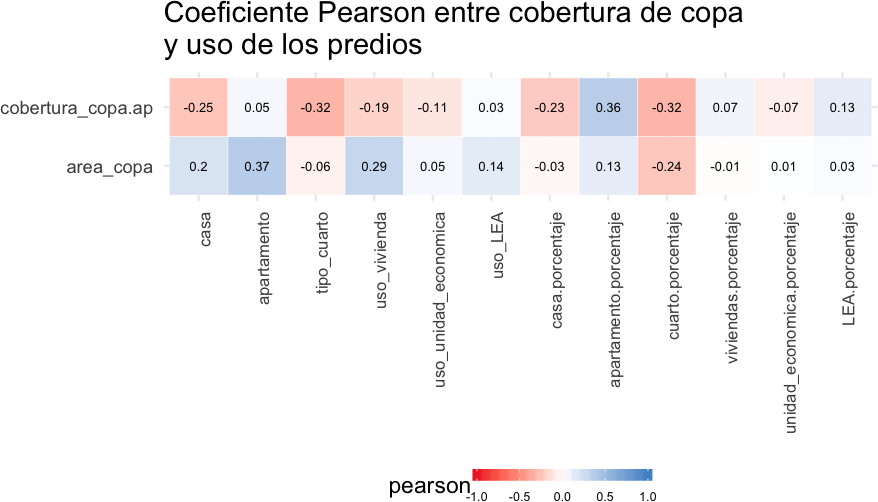
\includegraphics[width=1\linewidth]{tesis-unigis_files/figure-latex/tile-copa-prediosev-pearson-1} \caption{Coeficiente Pearson entre coberturas de copa
 y variables de predios y EV}\label{fig:tile-copa-prediosev-pearson}
\end{figure}

\begin{figure}
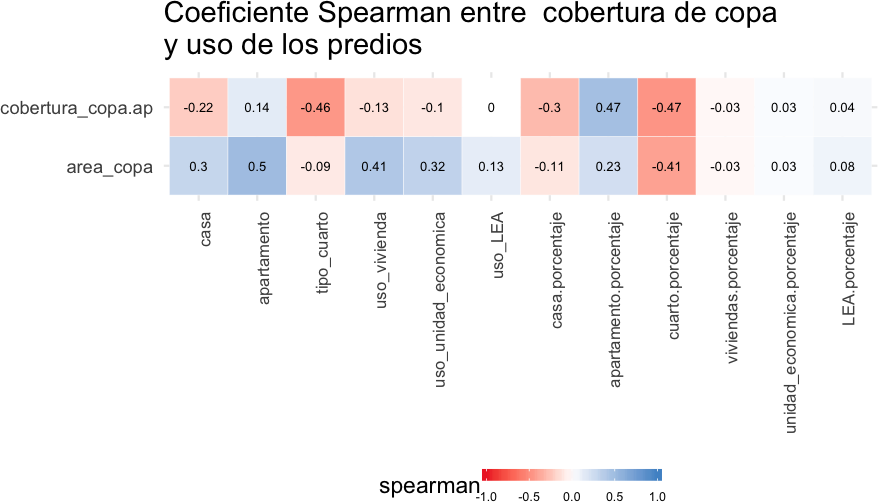
\includegraphics[width=1\linewidth]{tesis-unigis_files/figure-latex/tile-copa-prediosev-spearman-1} \caption{Coeficiente Pearson entre coberturas de copa
 y variables de predios y EV}\label{fig:tile-copa-prediosev-spearman}
\end{figure}

\subsection{Modelos de regresión
lineal}\label{modelos-de-regresion-lineal}

Antes de evaluar los modelos se aplicaron varias transformaciones en
busca de normalizar las distribuciones de las variables dependientes.
Las que mejor resultado arrojaron en la formulación de los modelos
fueron la transformación logarítmica para el caso de el área de copa y
la variable sin transformar en el caso de la cobertura de copa. A
continuación se presentan los resultados de los modelos de regresión

La tabla \ref{tab:coef-lm-copa} resume los coeficientes de la regresión
para la cobertura de copa.

\begin{table}

\caption{\label{tab:coef-lm-copa}Coeficientes OLS de área de copa - Log(AC)}
\centering
\begin{tabular}[t]{lrrrr}
\toprule
  & Estimate & Std. Error & t value & Pr(>|t|)\\
\midrule
(Intercept) & 0.788 & 0.013 & 62.256 & 0.000\\
superior\_postgrado.mxn & 0.312 & 0.024 & 13.013 & 0.000\\
densidad\_poblacion.mxn & -0.146 & 0.020 & -7.283 & 0.000\\
con\_alguna\_limitacion.porcentaje.mxn & -0.020 & 0.025 & -0.813 & 0.417\\
afro.porcentaje.mxn & 0.010 & 0.021 & 0.481 & 0.631\\
\addlinespace
cuarto.porcentaje.mxn & -0.145 & 0.030 & -4.754 & 0.000\\
area\_ep.mxn & 0.119 & 0.028 & 4.310 & 0.000\\
\bottomrule
\end{tabular}
\end{table}

La tabla \ref{tab:coef-lm-cobertura} resume los coeficientes de la
regresión para la cobertura de copa.

\begin{table}

\caption{\label{tab:coef-lm-cobertura}Coeficientes OLS de cobertura de copa - (CC)}
\centering
\begin{tabular}[t]{lrrrr}
\toprule
  & Estimate & Std. Error & t value & Pr(>|t|)\\
\midrule
(Intercept) & 0.03438 & 0.03989 & 0.86174 & 0.38948\\
superior\_postgrado.porcentaje.mxn & 0.38210 & 0.04227 & 9.03961 & 0.00000\\
densidad\_poblacion.mxn & 0.05573 & 0.03750 & 1.48613 & 0.13824\\
con\_alguna\_limitacion.porcentaje.mxn & 0.05848 & 0.04470 & 1.30827 & 0.19173\\
afro.porcentaje.mxn & -0.02170 & 0.04410 & -0.49201 & 0.62306\\
\addlinespace
apartamento.porcentaje.mxn & -0.04561 & 0.03547 & -1.28581 & 0.19945\\
cuarto.porcentaje.mxn & -0.06197 & 0.06163 & -1.00545 & 0.31545\\
area\_ep.porcentaje.mxn & 0.03971 & 0.03796 & 1.04619 & 0.29627\\
\bottomrule
\end{tabular}
\end{table}

La tabla \ref{tab:ajuste-lmcopa-pob-predios} resume las métricas de
ajuste de ambos modelos

\begin{table}

\caption{\label{tab:ajuste-lmcopa-pob-predios}Resumen métricas de ajuste OLS para el área de copa (AC) y cobertura de copa (CC) }
\centering
\begin{tabular}[t]{l|r|r}
\hline
medidasfit & Log(AC) & \%CC\\
\hline
Shapiro-Wilk & 0.98196 & 0.90416\\
\hline
SW p-value & 0.00043 & 0.00000\\
\hline
Breusch-Pagan & 21.62587 & 19.67634\\
\hline
BP p-value & 0.00142 & 0.00631\\
\hline
Media Residuos & 0.00000 & 0.00000\\
\hline
MSE & 0.00345 & 0.01071\\
\hline
adj-Rsquare & 0.60479 & 0.45931\\
\hline
AIC & -901.82032 & -532.26094\\
\hline
Log likelihood & 458.91016 & 275.13047\\
\hline
\end{tabular}
\end{table}

Ignoraremos las variables no significativas de los modelos lineales,
para los siguientes pasos de la metodología.

Existe no normalidad en los residuos y posibles no linealidades, como se
observa en las gráficas diagnósticas de la regresión
\ref{fig:diagn-mod-best-lm-copa}.

\begin{figure}
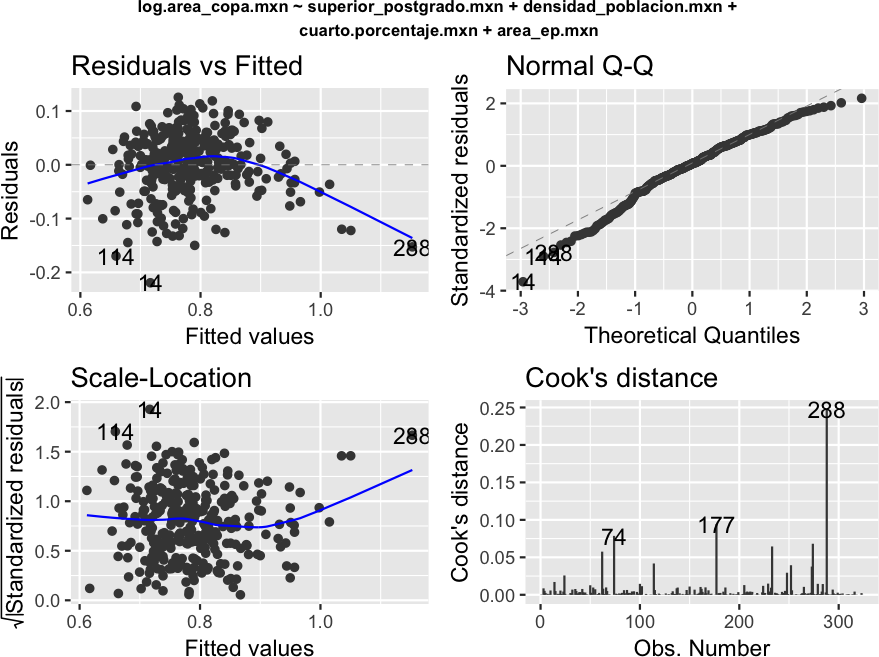
\includegraphics[width=1\linewidth]{tesis-unigis_files/figure-latex/diagn-mod-best-lm-copa-1} \caption{Gráficas diagnósticas para el análisis de regresión lineal de área de copa con los nuevos términos}\label{fig:diagn-mod-best-lm-copa}
\end{figure}

\begin{figure}
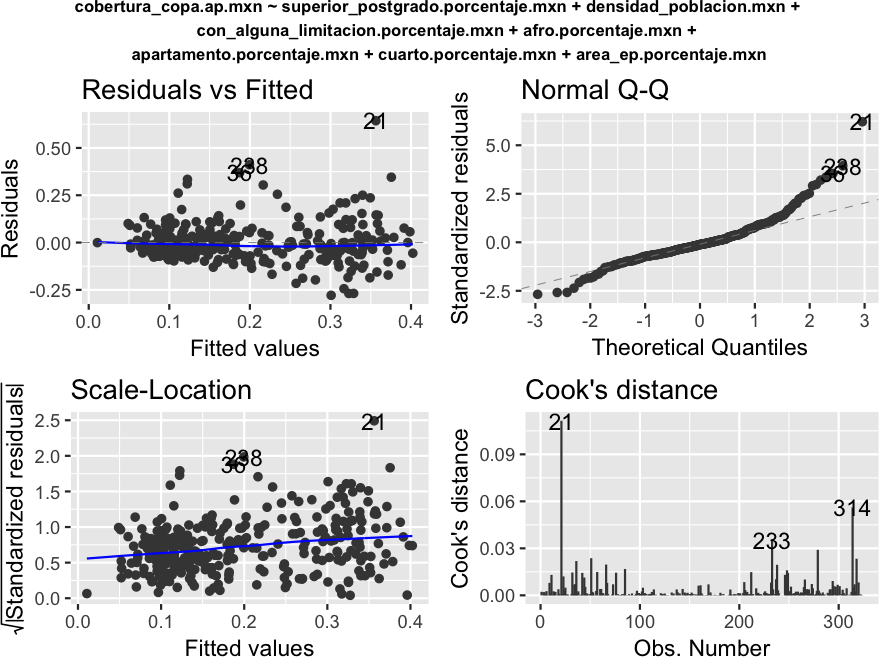
\includegraphics[width=1\linewidth]{tesis-unigis_files/figure-latex/diagn-mod-best-lm-copaap-1} \caption{Gráficas diagnósticas para el análisis de regresión lineal de porcentaje de cobertura de copa}\label{fig:diagn-mod-best-lm-copaap}
\end{figure}

Finalmente se presentan los mapas de las variables dependientes de los 2
modelos seleccionados, comparándolas con el modelo ajustado y los
residuos del ajuste, con el fin de observar donde se localizan los
errores en la predicción. La figura \ref{fig:mapas-lm-copa} corresponde
al ajuste del área de copa y la figura \ref{fig:mapas-lm-copaap} al
porcentaje de la cobertura de copa.

\begin{figure}
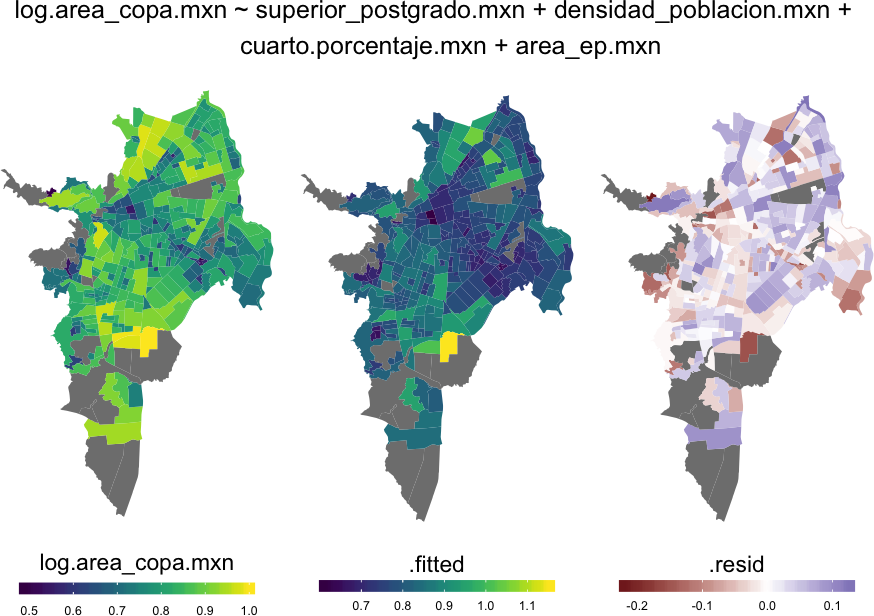
\includegraphics[width=1\linewidth]{tesis-unigis_files/figure-latex/mapas-lm-copa-1} \caption{Variable dependiente, valor ajustado por el modelo y residuos del OLS para log.area copa normalizada}\label{fig:mapas-lm-copa}
\end{figure}

\begin{figure}
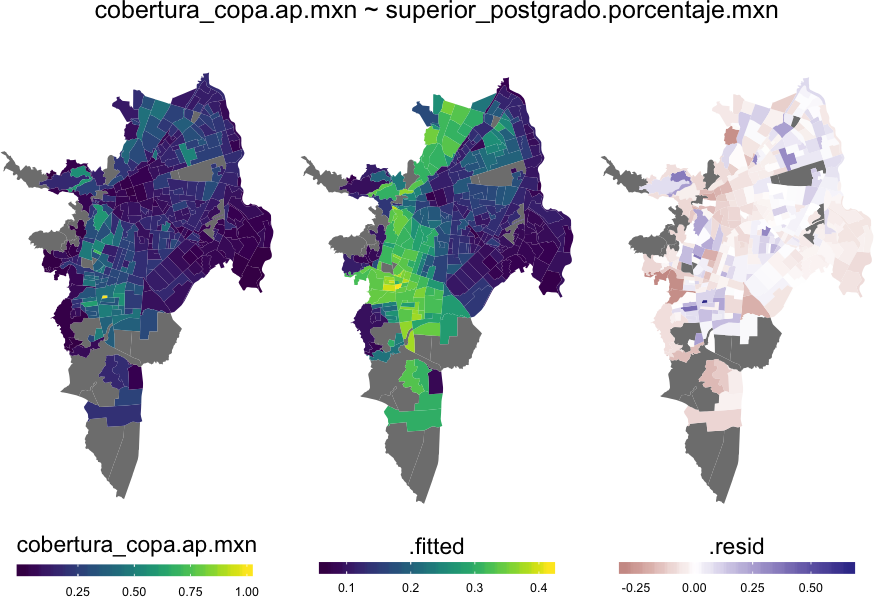
\includegraphics[width=1\linewidth]{tesis-unigis_files/figure-latex/mapas-lm-copaap-1} \caption{Variable dependiente, valor ajsutado por el modelo y residuos del OLS para cobertura copa.ap normalizada}\label{fig:mapas-lm-copaap}
\end{figure}

\subsection{Modelado espacial AU}\label{modelado-espacial-au}

Las matrices de vecindad construidas para el análisis espacial son la
\emph{queen} \(W_q\), que considera vecino a todos los sectores que
comparten un lado o una esquina con un sector censal; y una matriz de
distancia inversas entre los centroides de los SU, restringiendo la
vecindad a aquellos centroides que están a menos de 1 km (\(W_d\)). El
valor de un kilómetro es arbitrario, aunque razonable en la escala
humana. Los grafos que representan las 2 matrices \(W\) se muestran en
la figura \ref{fig:ws-su-reg}.

\begin{figure}

{\centering 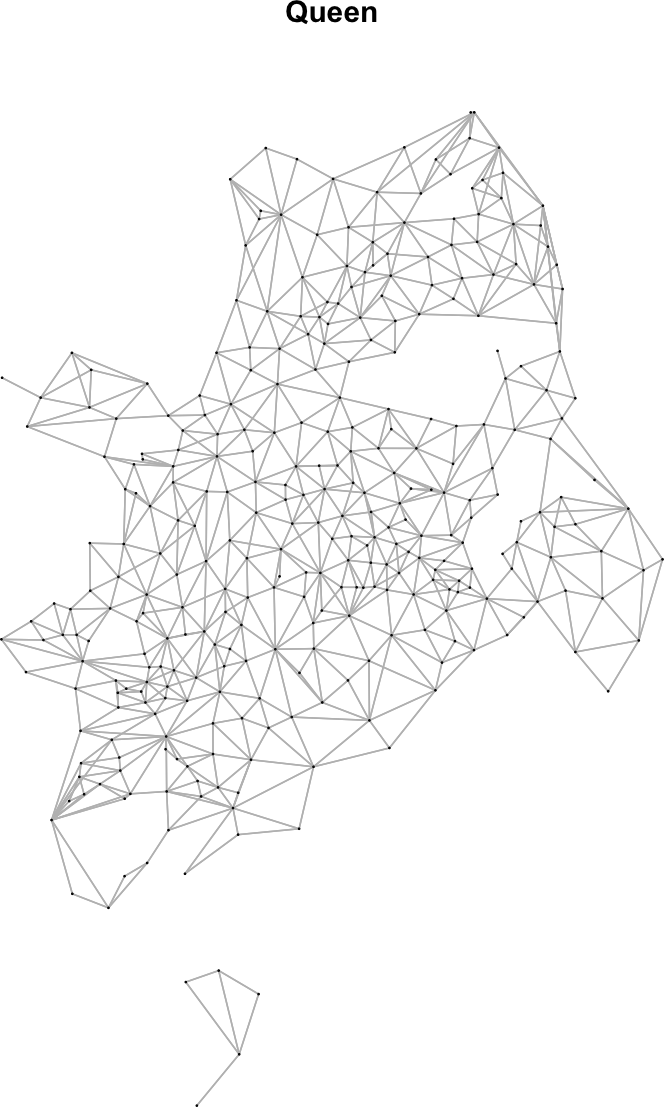
\includegraphics[width=0.48\linewidth]{tesis-unigis_files/figure-latex/ws-su-reg-1} 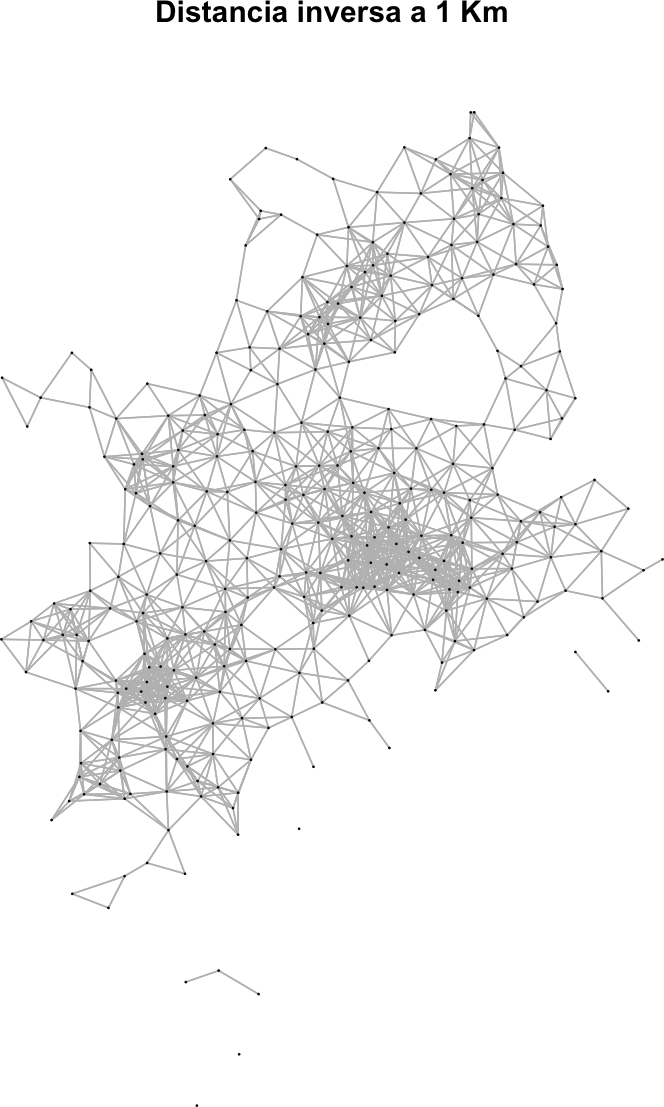
\includegraphics[width=0.48\linewidth]{tesis-unigis_files/figure-latex/ws-su-reg-2} 

}

\caption{Matrices de vecindad del análisis espacial}\label{fig:ws-su-reg}
\end{figure}

Examinemos primero la autocorrelación de las variables dependientes.

\subsubsection{Autocorrelación variables
dependientes}\label{autocorrelacion-variables-dependientes}

\begin{table}

\caption{\label{tab:moran-copa-wq}Test de Moran - Área de copa $W_q$}
\centering
\begin{tabular}[t]{lr}
\toprule
  &  \\
\midrule
Moran I statistic & 0.37488\\
Expectation & -0.00310\\
Variance & 0.00119\\
Moran I statistic standard deviate & 10.95802\\
p-value & 0.00000\\
\bottomrule
\end{tabular}
\end{table}

\begin{table}

\caption{\label{tab:moran-copa-wd}Test de Moran - Área de copa $W_d$}
\centering
\begin{tabular}[t]{lr}
\toprule
  &  \\
\midrule
Moran I statistic & 0.28174\\
Expectation & -0.00312\\
Variance & 0.00090\\
Moran I statistic standard deviate & 9.50984\\
p-value & 0.00000\\
\bottomrule
\end{tabular}
\end{table}

\begin{figure}
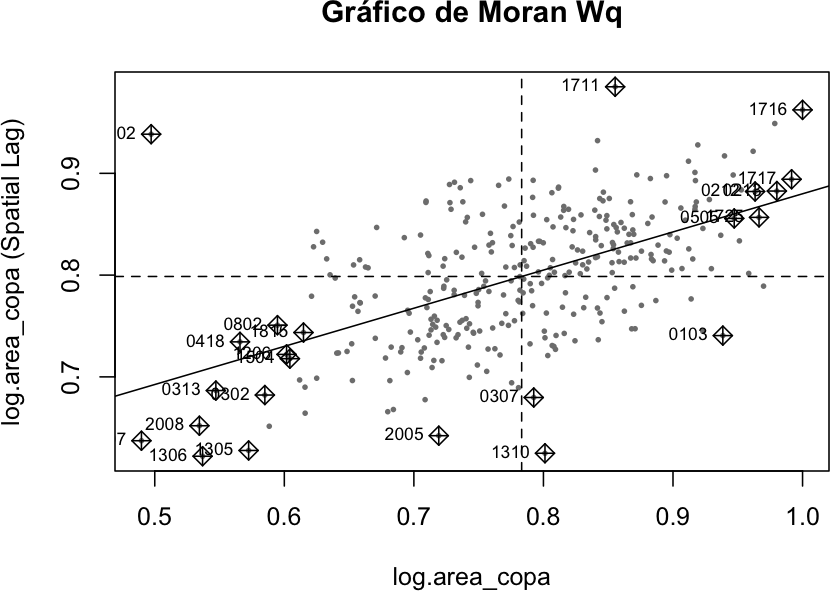
\includegraphics[width=0.49\linewidth]{tesis-unigis_files/figure-latex/moranplot-copa-w-1} 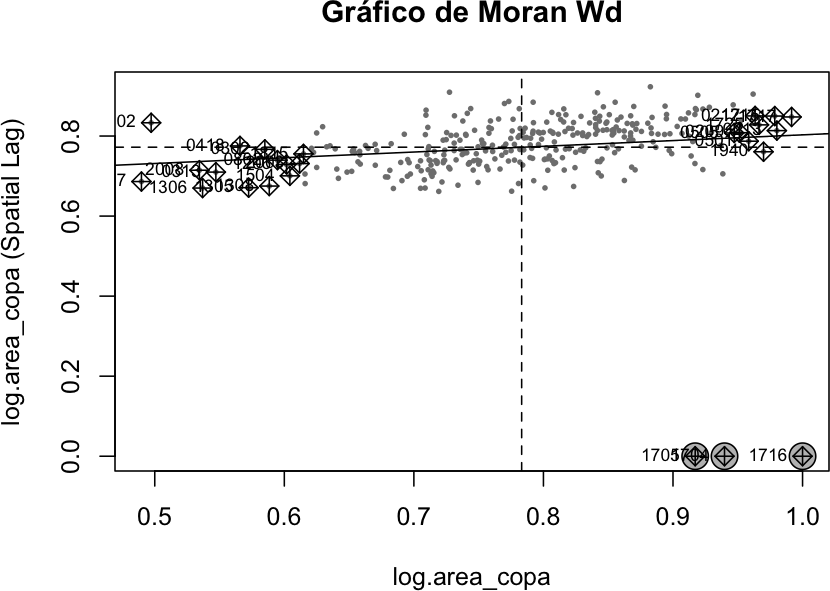
\includegraphics[width=0.49\linewidth]{tesis-unigis_files/figure-latex/moranplot-copa-w-2} \caption{Gráfico de Moran para los residuos del modelo lineal para del área de cobertura de copa usando $W_{q}$}\label{fig:moranplot-copa-w}
\end{figure}

La matriz \(W_q\) captura mucho mejor de forma global la autocorrelación
del área de copa. Los mapas LISA muestran los focos de esta
autocorrelación usando la matriz para \(W_q\) (figura
\ref{fig:mapas-lisa-copa-wq}) y para \(W_d\) (figura
\ref{fig:mapas-lisa-copa-wd}) .

\begin{figure}
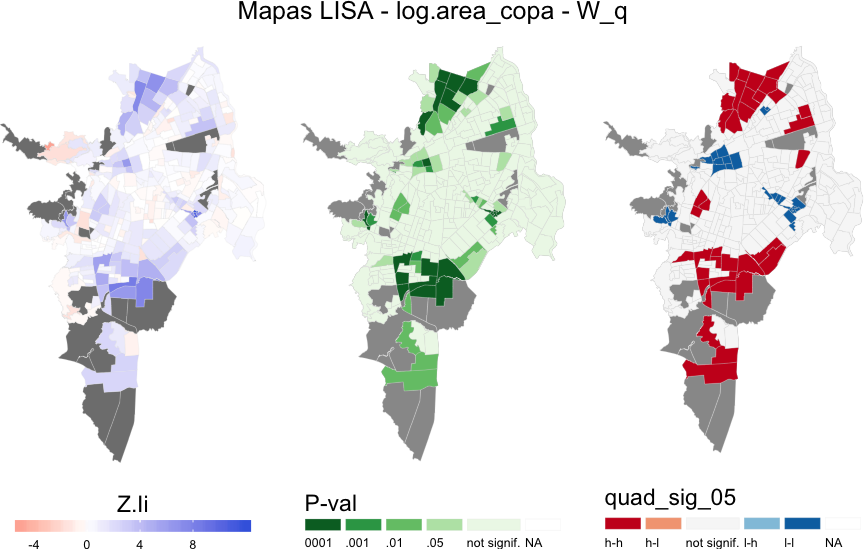
\includegraphics[width=1\linewidth]{tesis-unigis_files/figure-latex/mapas-lisa-copa-wq-1} \caption{Mapas LISA para la matriz $W_q$ de `log.area copa`}\label{fig:mapas-lisa-copa-wq}
\end{figure}

En los estos mapas de LISA de ambas matrices se observan que los
sectores en rojo (H-H) y azul (L-L) identifican los lugares con
autocorrelación positiva, formando grupos. No se presentan valores
negativos de autocorrelación.

\begin{figure}
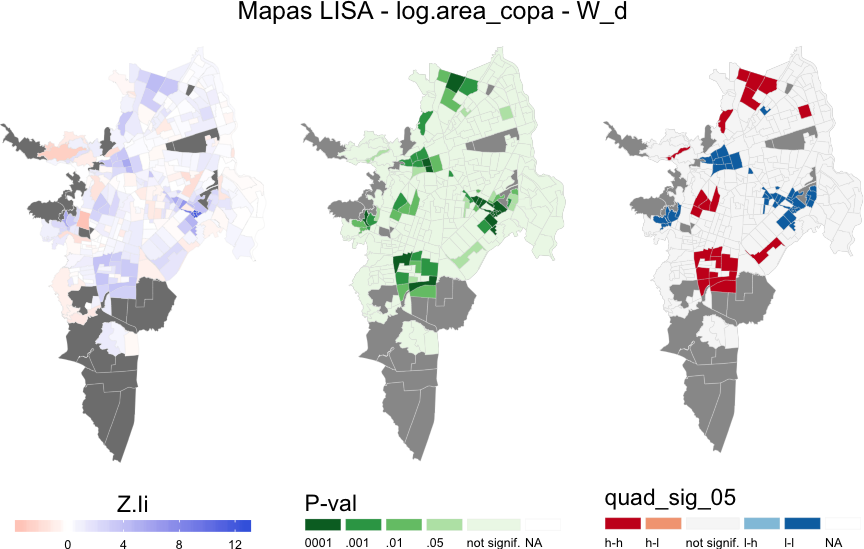
\includegraphics[width=1\linewidth]{tesis-unigis_files/figure-latex/mapas-lisa-copa-wd-1} \caption{Mapas LISA para la matriz $W_d$ de `log.area copa`}\label{fig:mapas-lisa-copa-wd}
\end{figure}

Para la variable dependiente porcentaje de cobertura de copa los
resultados del análisis de autocorrelación se presentan a continuación.

\begin{table}

\caption{\label{tab:moran-copaap-wq}Test de Moran - Cobertura de área de copa $W_q$}
\centering
\begin{tabular}[t]{lr}
\toprule
  &  \\
\midrule
Moran I statistic & 0.48104\\
Expectation & -0.00310\\
Variance & 0.00118\\
Moran I statistic standard deviate & 14.10670\\
p-value & 0.00000\\
\bottomrule
\end{tabular}
\end{table}

\begin{table}

\caption{\label{tab:moran-copaap-wd}Test de Moran - Cobertura de área de copa $W_d$}
\centering
\begin{tabular}[t]{lr}
\toprule
  &  \\
\midrule
Moran I statistic & 0.50225\\
Expectation & -0.00312\\
Variance & 0.00089\\
Moran I statistic standard deviate & 16.95747\\
p-value & 0.00000\\
\bottomrule
\end{tabular}
\end{table}

\begin{figure}
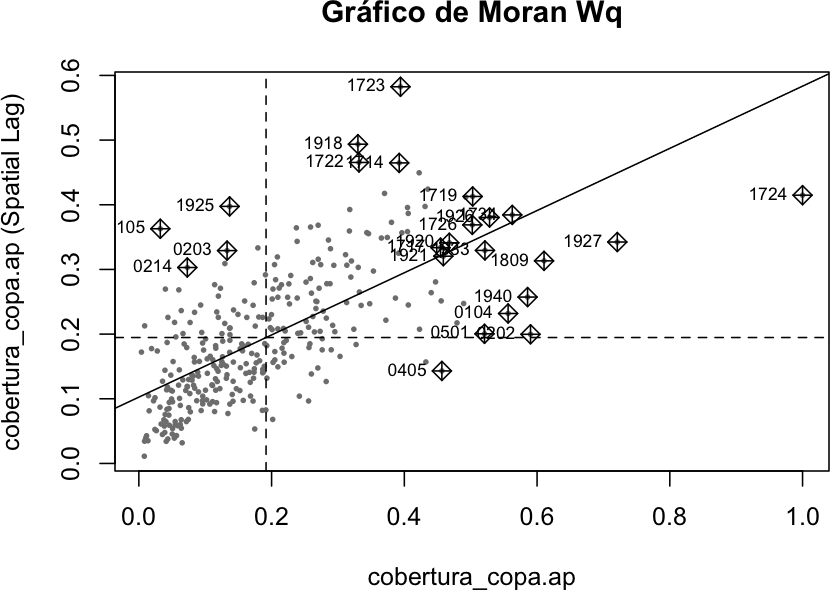
\includegraphics[width=0.49\linewidth]{tesis-unigis_files/figure-latex/moranplot-copaap-w-1} 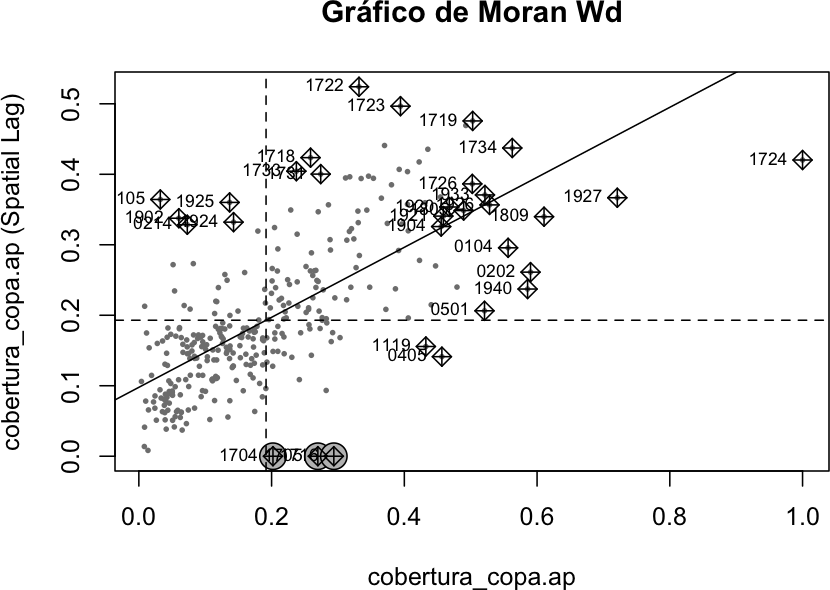
\includegraphics[width=0.49\linewidth]{tesis-unigis_files/figure-latex/moranplot-copaap-w-2} \caption{Gráfico de Moran para los residuos del modelo lineal para el porcentajes cobertura de copa usando $W_{q}$}\label{fig:moranplot-copaap-w}
\end{figure}

Ambos diseños de matriz revelan presencia clara de autocorrelación
espacial, pero la matrix \(W_d\) la captura ligeramente mejor con un
valor positivo y significativa, produciendo \emph{clusters} de sectores
urbanos más con más sectores urbanos. Los mapas LISA muestran los focos
de esta autocorrelación usando la matriz para \(W_q\) (figura
\ref{fig:mapas-lisa-copaap-wq}) y para \(W_d\) (figura
\ref{fig:mapas-lisa-copaap-wd}) . No se presentan valores negativos de
autocorrelación.

\begin{figure}
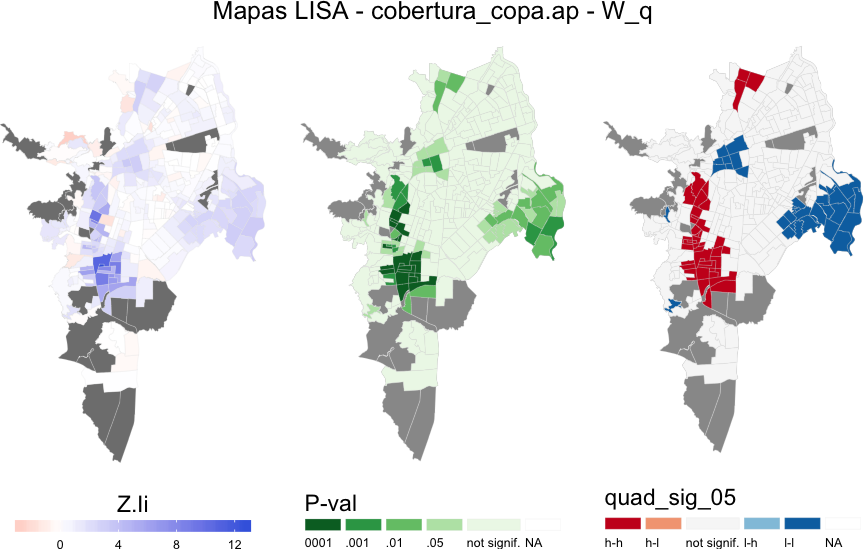
\includegraphics[width=1\linewidth]{tesis-unigis_files/figure-latex/mapas-lisa-copaap-wq-1} \caption{Mapas LISA para la matriz $W_q$ de `cobertura copa.ap`}\label{fig:mapas-lisa-copaap-wq}
\end{figure}

\begin{figure}
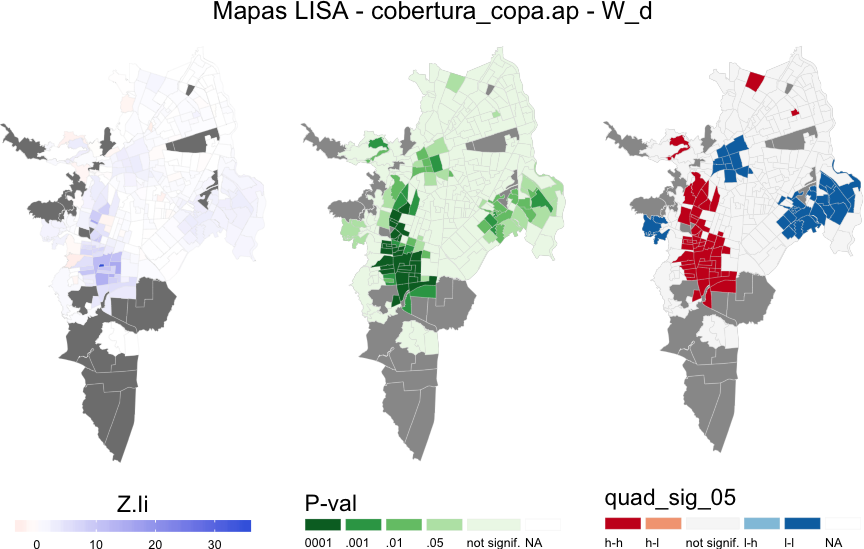
\includegraphics[width=1\linewidth]{tesis-unigis_files/figure-latex/mapas-lisa-copaap-wd-1} \caption{Mapas LISA para la matriz $W_d$ de `cobertura copa.ap`}\label{fig:mapas-lisa-copaap-wd}
\end{figure}

\subsubsection{Autocorrelación residuos de los
OLS}\label{autocorrelacion-residuos-de-los-ols}

El siguiente código calcula los índices de autocorrelación de los
residuos del mejor modelo lineal de área de copa
(\texttt{sqrt.copa\_area.mxn\ \textasciitilde{}\ superior\_postgrado.mxn\ +\ densidad\_poblacion.mxn\ +\ con\_alguna\_limitacion.porcentaje.mxn\ +\ afro.porcentaje.mxn\ +\ cuarto.porcentaje.mxn\ +\ area\_ep.mxn})
para ambas matrices \(W\) y construye los gráficos de Moran y mapas LISA
\ref{fig:moranplot-rescopa-w} para \(W_q\) y para \(W_d\).

\begin{table}

\caption{\label{tab:moran-rescopa-wq}Test de Moran - Residuos OLS área de copa $W_q$}
\centering
\begin{tabular}[t]{lr}
\toprule
  &  \\
\midrule
Observed Moran I & 0.09117\\
Expectation & -0.01124\\
Variance & 0.00115\\
Moran I statistic standard deviate & 3.02350\\
 & 0.00250\\
\bottomrule
\end{tabular}
\end{table}

\begin{table}

\caption{\label{tab:moran-rescopa-wd}Test de Moran - Residuos OLS área de copa $W_d$}
\centering
\begin{tabular}[t]{lr}
\toprule
  &  \\
\midrule
Observed Moran I & 0.11258\\
Expectation & -0.00955\\
Variance & 0.00085\\
Moran I statistic standard deviate & 4.17973\\
p-value & 0.00003\\
\bottomrule
\end{tabular}
\end{table}

\begin{figure}
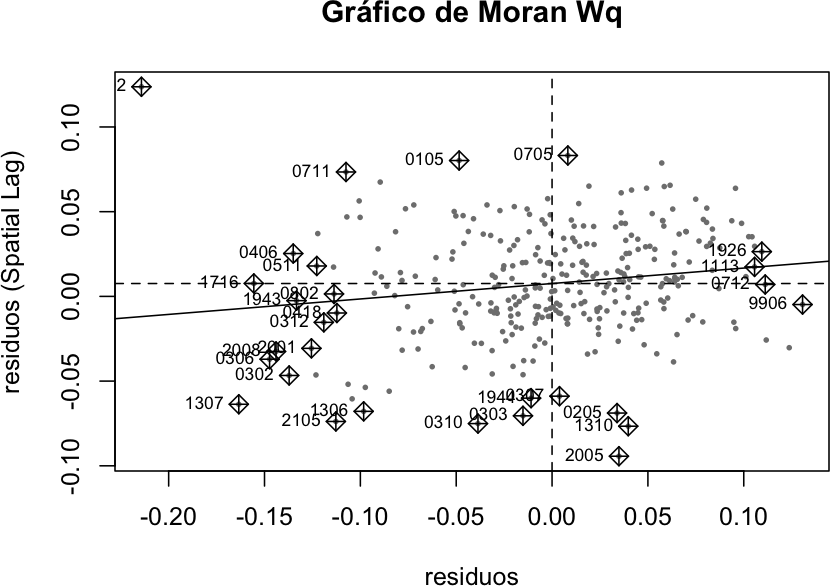
\includegraphics[width=0.49\linewidth]{tesis-unigis_files/figure-latex/moranplot-rescopa-w-1} 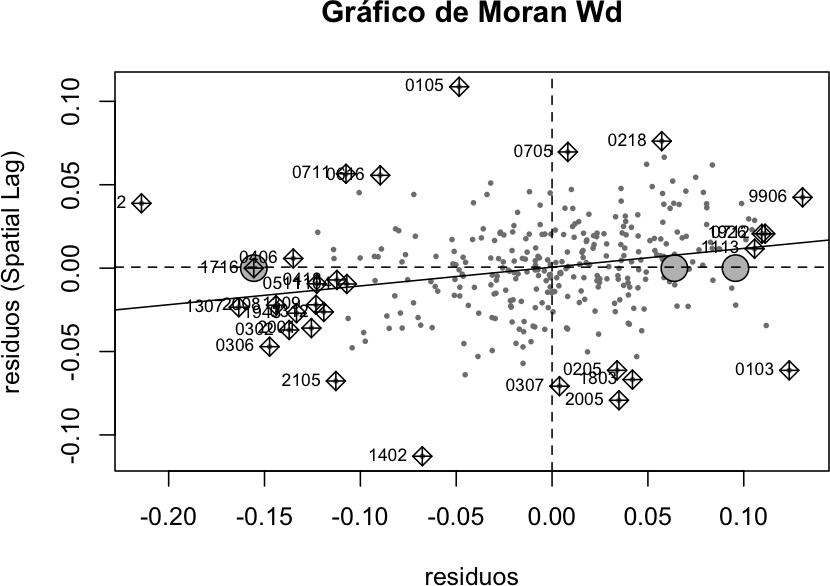
\includegraphics[width=0.49\linewidth]{tesis-unigis_files/figure-latex/moranplot-rescopa-w-2} \caption{Gráfico de Moran para los residuos del modelo lineal para del área de cobertura de copa usando $W_{q}$ y $W_{d}$ }\label{fig:moranplot-rescopa-w}
\end{figure}

Para ambos casos el valor de Moran Global es mayor que 0 y
significativo, aunque no es muy alto, si existe una tendencia en los
datos y ambas matrices capturan el efecto. \(W_d\) lo hace mejor en los
residuos, mientras \(W_q\) lo hace mejor con la variable dependiente. En
las figuras \ref{fig:mapas-lisa-rescopa-wq} y
\ref{fig:mapas-lisa-rescopa-wd} observamos que los grupos de sectores
son más pequeños que los de las variables dependientes, lo que podría
deberse a que las variables independientes presentan un patrón espacial
similar, y que por consiguiente, al introducir estos retardos al modelo
van a ayudar a absorber esa diferencias para mejorar la estimación.

\begin{figure}
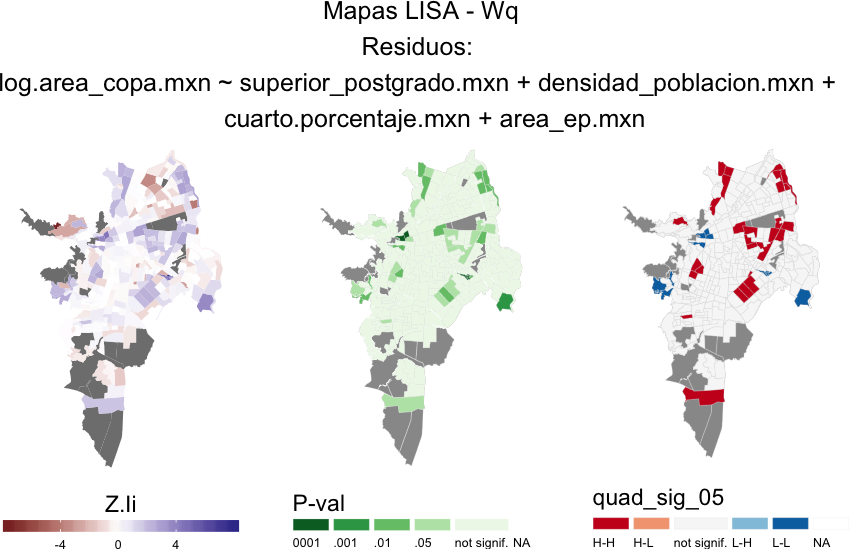
\includegraphics[width=1\linewidth]{tesis-unigis_files/figure-latex/mapas-lisa-rescopa-wq-1} \caption{Mapas LISA para la matriz $W_q$ de los residuos del modelo lineal para del área de copa}\label{fig:mapas-lisa-rescopa-wq}
\end{figure}

\begin{figure}
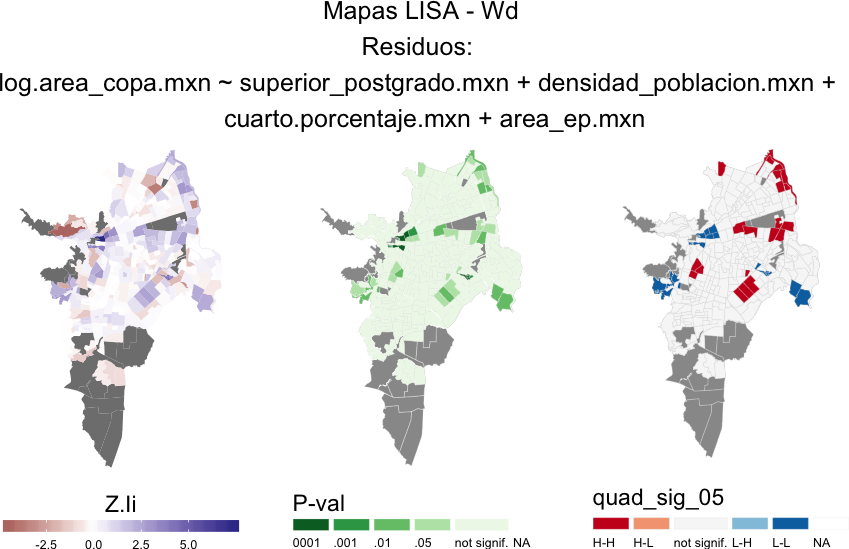
\includegraphics[width=1\linewidth]{tesis-unigis_files/figure-latex/mapas-lisa-rescopa-wd-1} \caption{Mapas LISA para la matriz $W_d$ dede los residuos del modelo lineal para del área de copa}\label{fig:mapas-lisa-rescopa-wd}
\end{figure}

El mismo análisis se aplica al modelo de porcentaje de cobertura de copa
(\texttt{cobertura\_copa.ap.mxn\ \textasciitilde{}\ superior\_postgrado.porcentaje.mxn}).

\begin{table}

\caption{\label{tab:moran-rescopaap-wq}Test de Moran - Residuos OLS cobertura de área de copa $W_q$}
\centering
\begin{tabular}[t]{lr}
\toprule
  &  \\
\midrule
Observed Moran I & 0.19436\\
Expectation & -0.00546\\
Variance & 0.00118\\
Moran I statistic standard deviate & 5.81914\\
p-value & 0.00000\\
\bottomrule
\end{tabular}
\end{table}

\begin{table}

\caption{\label{tab:moran-rescopaap-wd}Test de Moran - Residuos OLS cobertura de área de copa $W_d$}
\centering
\begin{tabular}[t]{lr}
\toprule
  &  \\
\midrule
Observed Moran I & 0.18821\\
Expectation & -0.00532\\
Variance & 0.00089\\
Moran I statistic standard deviate & 6.50277\\
p-value & 0.00000\\
\bottomrule
\end{tabular}
\end{table}

\begin{figure}
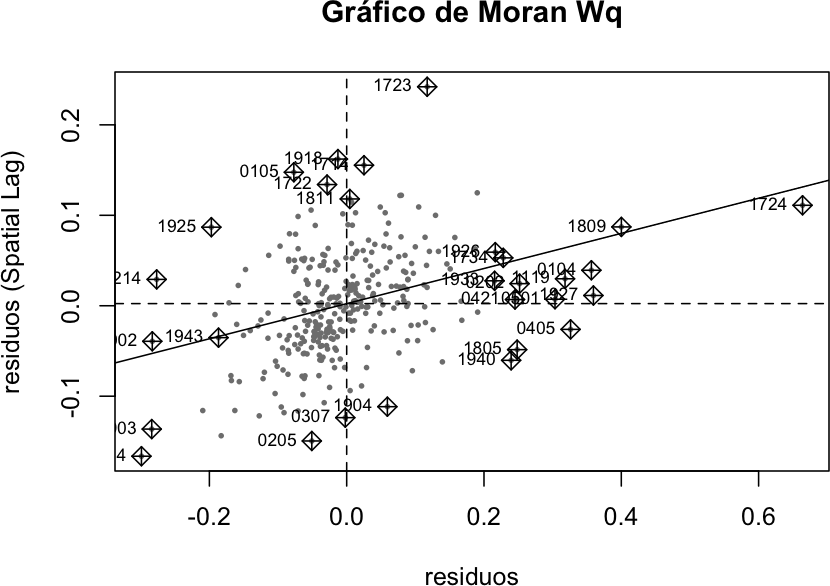
\includegraphics[width=0.49\linewidth]{tesis-unigis_files/figure-latex/moranplot-rescopaap-w-1} 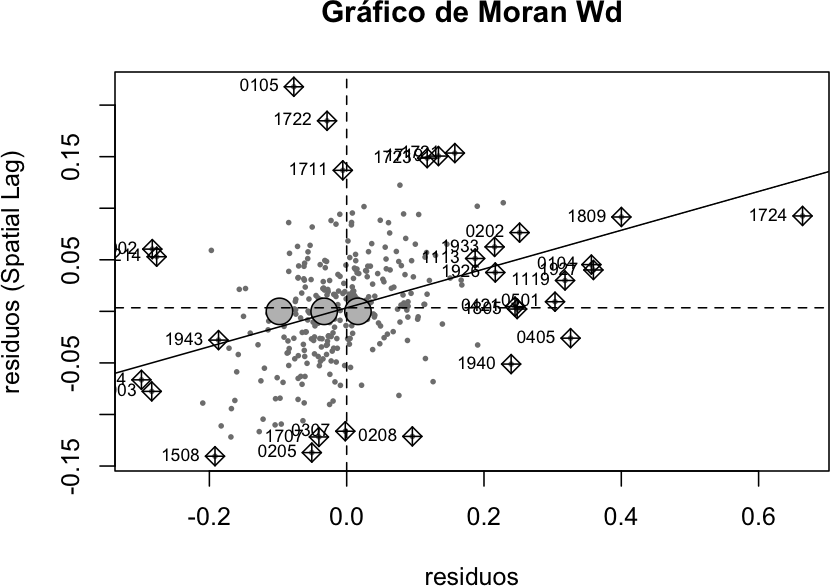
\includegraphics[width=0.49\linewidth]{tesis-unigis_files/figure-latex/moranplot-rescopaap-w-2} \caption{Gráfico de Moran para los residuos del modelo lineal para el porcentaje de cobertura de copa usando $W_{q}$ y $W_{d}$}\label{fig:moranplot-rescopaap-w}
\end{figure}

Para ambas matrices el valor de Moran Global es mayor que 0 y
significativo, casi el doble más alto que para el modelo de área de
copa; el indicador porcentual de cobertura y el residuo del modelo para
ajustarlo muestra el mismo comprtamiento en la sensibilidad de las
matrices: el efecto es más fuerte con \(W_d\) para la variable
dependiente y levemente mayor con \(W_q\) en los residuos. En las
figuras \ref{fig:mapas-lisa-rescopaap-wq} y
\ref{fig:mapas-lisa-rescopaap-wd} una vez más observamos que los grupos
de sectores son más pequeños que los de las variables dependientes, lo
que, como dijimos, se debe a que las variables independientes presentan
un patrón espacial similar, y se espera que al introducir estos efectos
espaciales al modelo mejora la confiabilidad de la estimación.

\begin{figure}
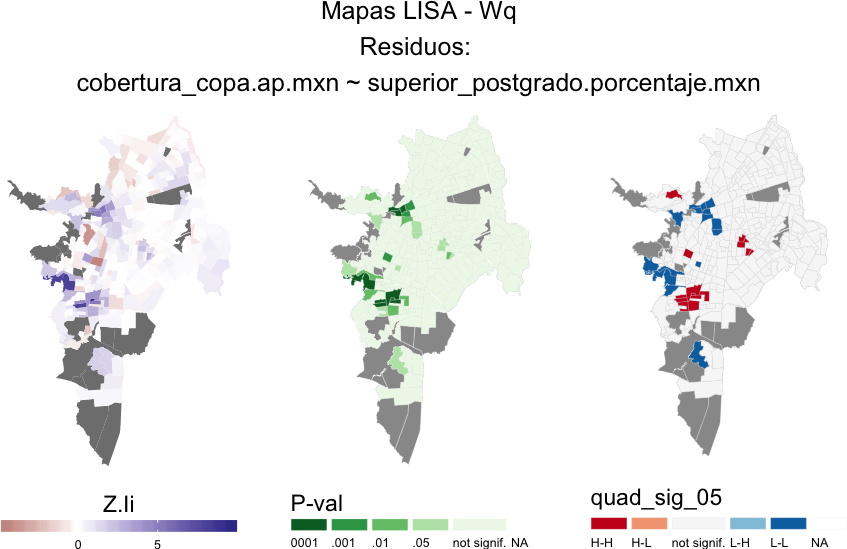
\includegraphics[width=1\linewidth]{tesis-unigis_files/figure-latex/mapas-lisa-rescopaap-wq-1} \caption{Mapas LISA para la matriz $W_q$ de los residuos del modelo lineal para el porcentaje de cobertura copa}\label{fig:mapas-lisa-rescopaap-wq}
\end{figure}

\begin{figure}
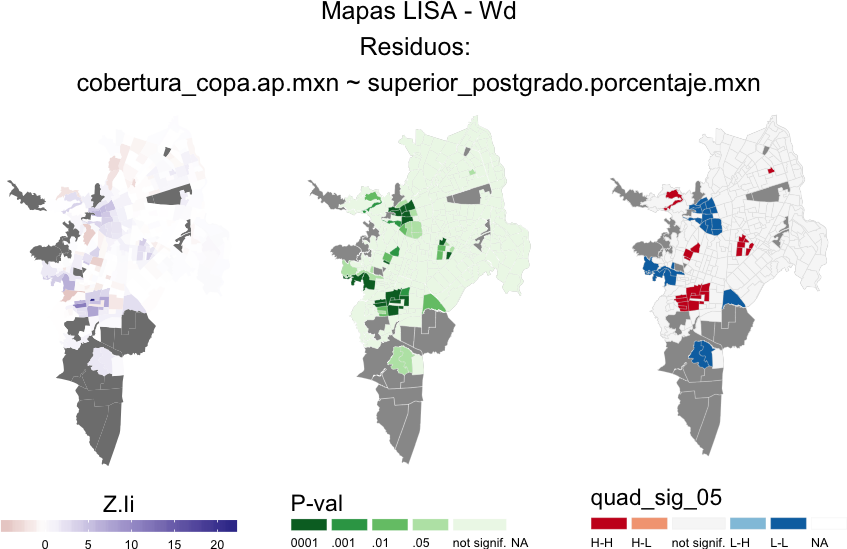
\includegraphics[width=1\linewidth]{tesis-unigis_files/figure-latex/mapas-lisa-rescopaap-wd-1} \caption{Mapas LISA para la matriz $W_d$ dede los residuos del modelo lineal para del área de copa}\label{fig:mapas-lisa-rescopaap-wd}
\end{figure}

Los resultados nos invitan a proceder a realizar un ajuste en ambos
modelos introduciendo algún tipo de estructura espacial. Posiblemente la
matriz \(W_q\) sea la candidata para el área de copa si se piensa en un
modelo autorregresivo, pues parece capturar mejor en los test de
autocorrelación global la existencia de grupos formados por fenómenos de
dispersión o derrame en la distribución de la copa. En el caso de usar
modelos de error espacial SEM posiblemente la candidata sea \(W_d\) por
capturar mejor la autocorrelación en los residuos.

\subsubsection{Modelo espacial área de
copa}\label{modelo-espacial-area-de-copa}

Para simplificar el análisis usaremos \(W_q\) ya que las diferencias no
son tan grandes entre ambas matrices. A continuación se presentan los
resultados del modelado de los 4 tipos de modelos geoestadísticos para
el área de copa.

\begin{table}

\caption{\label{tab:coef-sar-copa}Coeficientes del modelo SAR de área de copa}
\centering
\begin{tabular}[t]{lrrrr}
\toprule
  & Estimate & Std. Error & z value & Pr(>|z|)\\
\midrule
(Intercept) & 0.614 & 0.052 & 11.890 & 0.000\\
superior\_postgrado.mxn & 0.295 & 0.024 & 12.378 & 0.000\\
densidad\_poblacion.mxn & -0.125 & 0.020 & -6.192 & 0.000\\
con\_alguna\_limitacion.porcentaje.mxn & -0.011 & 0.024 & -0.446 & 0.656\\
afro.porcentaje.mxn & 0.015 & 0.020 & 0.746 & 0.455\\
\addlinespace
cuarto.porcentaje.mxn & -0.114 & 0.030 & -3.749 & 0.000\\
area\_ep.mxn & 0.113 & 0.027 & 4.202 & 0.000\\
\bottomrule
\end{tabular}
\end{table}

\begin{table}

\caption{\label{tab:cauto-sar-copa}Coeficiente de autocorrelación modelo SAR de área de copa}
\centering
\begin{tabular}[t]{lll}
\toprule
\$\textbackslash{}rho\$ & Likelihood ratio & p-value\\
0.202 & 11.788 & 0.001\\
\bottomrule
\end{tabular}
\end{table}

\begin{table}

\caption{\label{tab:coef-sem-copa}Coeficientes del modelo SEM de área de copa}
\centering
\begin{tabular}[t]{lrrrr}
\toprule
  & Estimate & Std. Error & z value & Pr(>|z|)\\
\midrule
(Intercept) & 0.781 & 0.014 & 57.469 & 0.000\\
superior\_postgrado.mxn & 0.303 & 0.024 & 12.485 & 0.000\\
densidad\_poblacion.mxn & -0.135 & 0.021 & -6.378 & 0.000\\
con\_alguna\_limitacion.porcentaje.mxn & -0.012 & 0.025 & -0.478 & 0.632\\
afro.porcentaje.mxn & -0.001 & 0.023 & -0.043 & 0.966\\
\addlinespace
cuarto.porcentaje.mxn & -0.130 & 0.033 & -3.993 & 0.000\\
area\_ep.mxn & 0.130 & 0.029 & 4.523 & 0.000\\
\bottomrule
\end{tabular}
\end{table}

\begin{table}

\caption{\label{tab:cauto-sem-copa}Coeficiente de autocorrelación modelo SEM de área de copa}
\centering
\begin{tabular}[t]{lll}
\toprule
\$\textbackslash{}lambda\$ & Likelihood ratio & p-value\\
6.466 & 0.011 & 6.466\\
\bottomrule
\end{tabular}
\end{table}

\begin{table}

\caption{\label{tab:coef-sd-copa}Coeficientes del modelo SD de área de copa}
\centering
\begin{tabular}[t]{lrrrr}
\toprule
  & Estimate & Std. Error & z value & Pr(>|z|)\\
\midrule
(Intercept) & 0.665 & 0.067 & 9.857 & 0.000\\
superior\_postgrado.mxn & 0.287 & 0.024 & 11.741 & 0.000\\
densidad\_poblacion.mxn & -0.088 & 0.026 & -3.431 & 0.001\\
con\_alguna\_limitacion.porcentaje.mxn & 0.007 & 0.027 & 0.273 & 0.785\\
afro.porcentaje.mxn & -0.041 & 0.040 & -1.013 & 0.311\\
\addlinespace
cuarto.porcentaje.mxn & -0.062 & 0.042 & -1.486 & 0.137\\
area\_ep.mxn & 0.134 & 0.030 & 4.455 & 0.000\\
lag.superior\_postgrado.mxn & 0.040 & 0.051 & 0.789 & 0.430\\
lag.densidad\_poblacion.mxn & -0.103 & 0.044 & -2.316 & 0.021\\
lag.con\_alguna\_limitacion.porcentaje.mxn & -0.060 & 0.046 & -1.292 & 0.196\\
\addlinespace
lag.afro.porcentaje.mxn & 0.116 & 0.051 & 2.268 & 0.023\\
lag.cuarto.porcentaje.mxn & -0.123 & 0.068 & -1.823 & 0.068\\
lag.area\_ep.mxn & -0.103 & 0.042 & -2.474 & 0.013\\
\bottomrule
\end{tabular}
\end{table}

\begin{table}

\caption{\label{tab:cauto-sd-copa}Coeficiente de autocorrelación modelo SD de área de copa}
\centering
\begin{tabular}[t]{lll}
\toprule
\$\textbackslash{}rho\$ & Likelihood ratio & p-value\\
0.175 & 4.82 & 0.028\\
\bottomrule
\end{tabular}
\end{table}

\begin{table}

\caption{\label{tab:coef-slx-copa}Coeficientes del modelo SLX de área de copa}
\centering
\begin{tabular}[t]{lrrrr}
\toprule
  & Estimate & Std. Error & t value & Pr(>|t|)\\
\midrule
x(Intercept) & 0.805 & 0.020 & 40.702 & 0.000\\
xsuperior\_postgrado.mxn & 0.287 & 0.025 & 11.431 & 0.000\\
xdensidad\_poblacion.mxn & -0.091 & 0.026 & -3.439 & 0.001\\
xcon\_alguna\_limitacion.porcentaje.mxn & 0.007 & 0.027 & 0.247 & 0.805\\
xafro.porcentaje.mxn & -0.039 & 0.041 & -0.950 & 0.343\\
\addlinespace
xcuarto.porcentaje.mxn & -0.067 & 0.043 & -1.553 & 0.121\\
xarea\_ep.mxn & 0.130 & 0.031 & 4.209 & 0.000\\
xlag.superior\_postgrado.mxn & 0.104 & 0.044 & 2.362 & 0.019\\
xlag.densidad\_poblacion.mxn & -0.131 & 0.044 & -2.989 & 0.003\\
xlag.con\_alguna\_limitacion.porcentaje.mxn & -0.069 & 0.048 & -1.458 & 0.146\\
\addlinespace
xlag.afro.porcentaje.mxn & 0.124 & 0.053 & 2.346 & 0.020\\
xlag.cuarto.porcentaje.mxn & -0.146 & 0.068 & -2.141 & 0.033\\
xlag.area\_ep.mxn & -0.084 & 0.042 & -1.973 & 0.049\\
\bottomrule
\end{tabular}
\end{table}

\begin{table}

\caption{\label{tab:tabla-comp-modelos-copa}Metricas de ajuste para los modelos de área de copa}
\centering
\begin{tabular}[t]{l|r|r|r|r|r}
\hline
medidasfit & OLS & SLX & SAR & SEM & SD\\
\hline
Globla Moran'I & 0.09117 & 0.07976 & -0.01715 & -0.01031 & -0.00695\\
\hline
GMI p-value & 0.00313 & 0.00816 & 0.65831 & 0.58286 & 0.54450\\
\hline
Shapiro-Wilk & 0.98196 & 0.99004 & 0.98107 & 0.97801 & 0.98845\\
\hline
SW p-value & 0.00043 & 0.02653 & 0.00028 & 0.00007 & 0.01121\\
\hline
Breusch-Pagan & 21.62587 & 34.78295 & 15.28709 & 14.33666 & 32.35172\\
\hline
BP p-value & 0.00142 & 0.00051 & 0.01814 & 0.02609 & 0.00122\\
\hline
Media Residuos & 0.00000 & 0.00000 & 0.00000 & 0.00000 & 0.00000\\
\hline
MSE & 0.00345 & 0.00322 & 0.00330 & 0.00335 & 0.00315\\
\hline
adj-Rsquare & 0.60479 & 0.99461 & NA & NA & NA\\
\hline
Nagelkerke pseudo-R-squared & NA & NA & 0.62599 & 0.61980 & 0.64283\\
\hline
AIC & -901.82032 & -911.71201 & -911.60831 & -906.28644 & -914.53237\\
\hline
Log likelihood & 458.91016 & 469.85601 & 464.80415 & 462.14322 & 472.26619\\
\hline
\end{tabular}
\end{table}

Al comparar los resultados de las métricas de ajuste se identifica al
modelo SD o mixto(variables con retardo y autocorrelación) con el mejor
AIC. El modelo SD ha logrado eliminar la autocorrelación espacial global
en los residuos, al igual que SAR y SEM (ver figura
\ref{fig:moranplot-resmodel-all-wq}). Aunque persiste la no normalidad
de los residuos y la heterocedasticidad como los muestran los test y las
gráficas diagnósticas, el error cometido disminuye y los coeficientes
pueden considerarse más confiables. El \(\rho\) y \(\lambda\) de las
estimaciones con términos de autorregresivos es significativo, lo que
implica que la inclusión de los retardos funciona correctamente, aunque
solo en los coeficientes de la variable retardada
\texttt{cuarto.porcentaje} es significativo, aunque esta no tiene un
coeficiente significativo como variable sin retardo, sugiriendo que
interesa su efecto sobre el área de copa en los sectores vecinos a los
focos de mayor concentración de viviendas tipo cuarto, pero no es
importante en el resto de sectores. Como era de esperarse el porcentaje
de área de espacios verdes es significativo en las variables sin
retardo, pero no genera ningún efecto de derrame en la cobertura de copa
de los sectores vecinos. A pesar de que los test de normalidad y
heterocedasticidad no son exitosos, las gráficas diagnósticas muestran
que los problemas se presentan en los valores extremos.

\begin{figure}
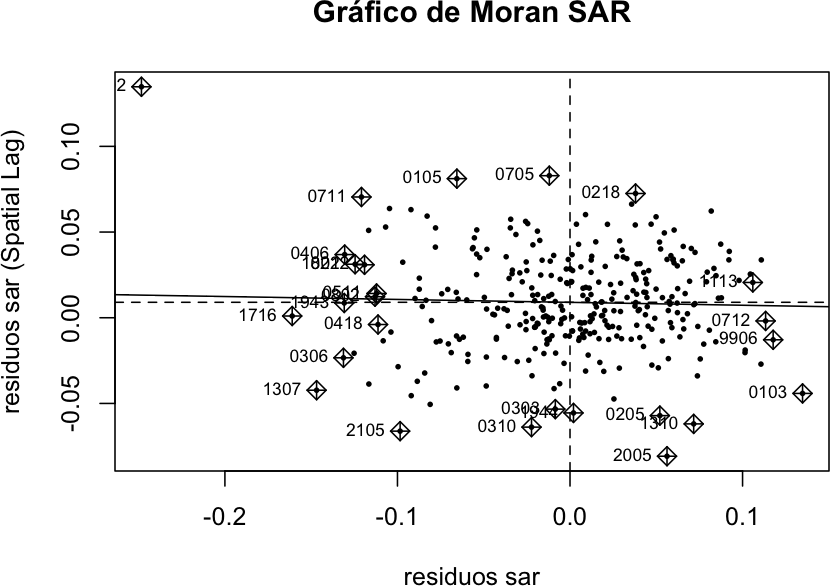
\includegraphics[width=0.49\linewidth]{tesis-unigis_files/figure-latex/moranplot-resmodel-all-wq-1} 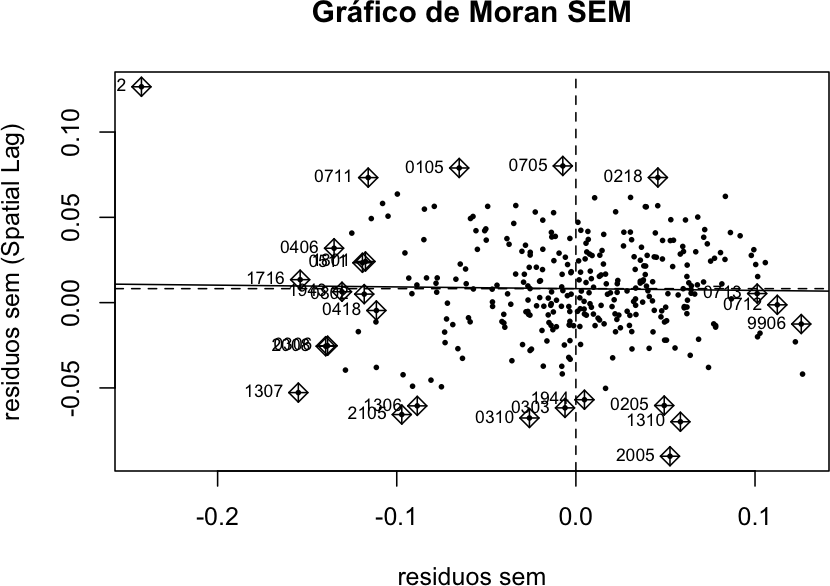
\includegraphics[width=0.49\linewidth]{tesis-unigis_files/figure-latex/moranplot-resmodel-all-wq-2} 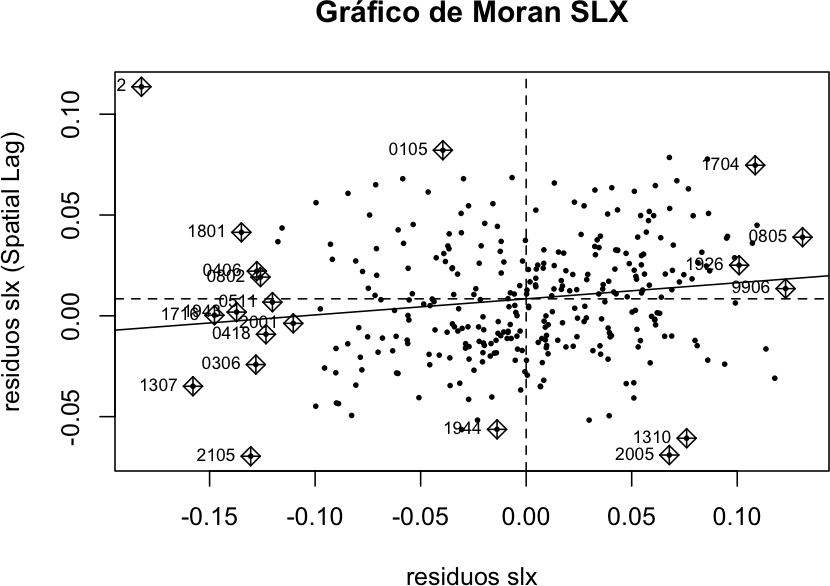
\includegraphics[width=0.49\linewidth]{tesis-unigis_files/figure-latex/moranplot-resmodel-all-wq-3} 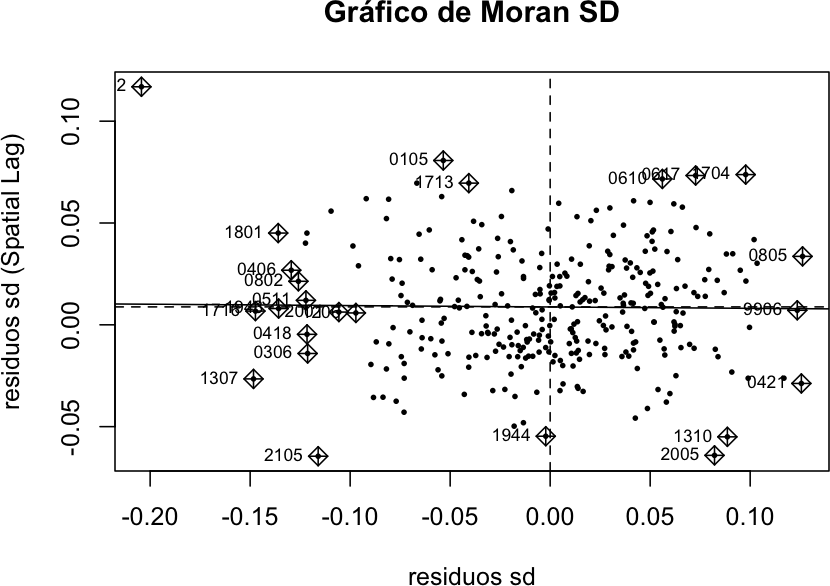
\includegraphics[width=0.49\linewidth]{tesis-unigis_files/figure-latex/moranplot-resmodel-all-wq-4} \caption{Gráfico de Moran para los residuos de los modelos espaciales de área de copa usando $W_{q}$}\label{fig:moranplot-resmodel-all-wq}
\end{figure}

\begin{figure}
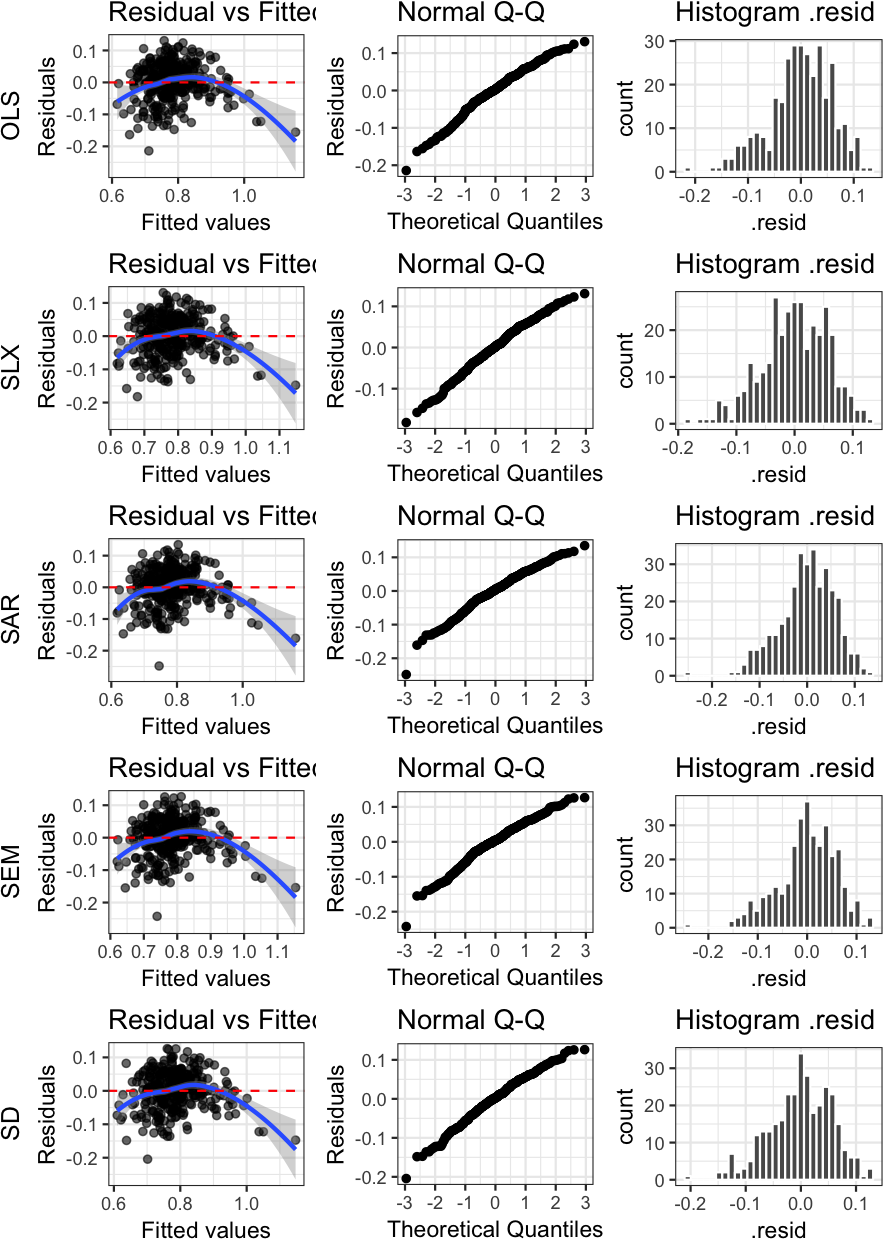
\includegraphics[width=1\linewidth]{tesis-unigis_files/figure-latex/diag-model-espaciales-1} \caption{Diagnóstico comparativo entre modelos}\label{fig:diag-model-espaciales}
\end{figure}

\subsubsection{Modelo espacial porcentaje de cobertura de área de
copa}\label{modelo-espacial-porcentaje-de-cobertura-de-area-de-copa}

El mismo ejercicio se aplica al porcentaje de cobertura de copa.

\begin{table}

\caption{\label{tab:coef-sar-copaap}Coeficientes del modelo SAR de porcentaje de área de copa}
\centering
\begin{tabular}[t]{lrrrr}
\toprule
  & Estimate & Std. Error & z value & Pr(>|z|)\\
\midrule
(Intercept) & 0.030 & 0.011 & 2.822 & 0.005\\
superior\_postgrado.porcentaje.mxn & 0.246 & 0.027 & 9.023 & 0.000\\
\bottomrule
\end{tabular}
\end{table}

\begin{table}

\caption{\label{tab:cauto-sar-copaap}Coeficiente de autocorrelación modelo SAR de porcentaje de área de copa}
\centering
\begin{tabular}[t]{lll}
\toprule
\$\textbackslash{}rho\$ & Likelihood ratio & p-value\\
0.375 & 28.579 & 0\\
\bottomrule
\end{tabular}
\end{table}

\begin{table}

\caption{\label{tab:coef-sem-copaap}Coeficientes del modelo SEM de porcentaje de área de copa}
\centering
\begin{tabular}[t]{lrrrr}
\toprule
  & Estimate & Std. Error & z value & Pr(>|z|)\\
\midrule
(Intercept) & 0.070 & 0.014 & 5.149 & 0\\
superior\_postgrado.porcentaje.mxn & 0.334 & 0.028 & 11.899 & 0\\
\bottomrule
\end{tabular}
\end{table}

\begin{table}

\caption{\label{tab:cauto-sem-copaap}Coeficiente de autocorrelación modelo SEM de porcentaje de área de copa}
\centering
\begin{tabular}[t]{lll}
\toprule
\$\textbackslash{}lambda\$ & Likelihood ratio & p-value\\
26.77 & 0 & 26.77\\
\bottomrule
\end{tabular}
\end{table}

\begin{table}

\caption{\label{tab:coef-sd-copaap}Coeficientes del modelo SD de porcentaje de área de copa}
\centering
\begin{tabular}[t]{lrrrr}
\toprule
  & Estimate & Std. Error & z value & Pr(>|z|)\\
\midrule
(Intercept) & 0.032 & 0.011 & 2.937 & 0.003\\
superior\_postgrado.porcentaje.mxn & 0.278 & 0.044 & 6.261 & 0.000\\
lag.superior\_postgrado.porcentaje.mxn & -0.051 & 0.058 & -0.880 & 0.379\\
\bottomrule
\end{tabular}
\end{table}

\begin{table}

\caption{\label{tab:cauto-sd-copaap}Coeficiente de autocorrelación modelo SD de porcentaje de área de copa}
\centering
\begin{tabular}[t]{lll}
\toprule
\$\textbackslash{}rho\$ & Likelihood ratio & p-value\\
0.401 & 27.538 & 0\\
\bottomrule
\end{tabular}
\end{table}

\begin{table}

\caption{\label{tab:coef-slx-copaap}Coeficientes del modelo SLX de porcentaje de área de copa}
\centering
\begin{tabular}[t]{lrrrr}
\toprule
  & Estimate & Std. Error & t value & Pr(>|t|)\\
\midrule
x(Intercept) & 0.059 & 0.011 & 5.472 & 0.000\\
xsuperior\_postgrado.porcentaje.mxn & 0.293 & 0.047 & 6.190 & 0.000\\
xlag.superior\_postgrado.porcentaje.mxn & 0.075 & 0.056 & 1.354 & 0.177\\
\bottomrule
\end{tabular}
\end{table}

\begin{table}

\caption{\label{tab:tabla-comp-modelos-copaap}Metricas de ajuste para los modelos de porcentaje de área de copa}
\centering
\begin{tabular}[t]{l|r|r|r|r|r}
\hline
medidasfit & OLS & SLX & SAR & SEM & SD\\
\hline
Globla Moran'I & 0.19436 & 0.19945 & 0.00734 & -0.01131 & -0.00863\\
\hline
GMI p-value & 0.00000 & 0.00000 & 0.37996 & 0.59509 & 0.56441\\
\hline
Shapiro-Wilk & 0.90492 & 0.90851 & 0.89936 & 0.89238 & 0.89685\\
\hline
SW p-value & 0.00000 & 0.00000 & 0.00000 & 0.00000 & 0.00000\\
\hline
Breusch-Pagan & 16.82734 & 16.80794 & 16.22458 & 15.21537 & 17.19946\\
\hline
BP p-value & 0.00004 & 0.00022 & 0.00006 & 0.00010 & 0.00018\\
\hline
Media Residuos & 0.00000 & 0.00000 & 0.00000 & 0.00000 & 0.00000\\
\hline
MSE & 0.01100 & 0.01094 & 0.00979 & 0.00981 & 0.00972\\
\hline
adj-Rsquare & 0.45512 & 0.80624 & NA & NA & NA\\
\hline
Nagelkerke pseudo-R-squared & NA & NA & 0.50267 & 0.49988 & 0.50390\\
\hline
AIC & -535.66434 & -535.50971 & -562.24323 & -560.43438 & -561.04776\\
\hline
Log likelihood & 270.83217 & 271.75485 & 285.12162 & 284.21719 & 285.52388\\
\hline
\end{tabular}
\end{table}

Al comparar los resultados de las métricas de ajuste se identifica al
modelo SAR con el mejor rendimiento en el ajuste del modelo. El
coeficiente de correlación \(\rho\) es alto y muy significativo, lo que
nos dice que es una mejora la inclusión de las características
espaciales en los datos, y se reflejados en el índice de Akaike que
tiene una mejora visible (de \(-535.6643429\) a \(-562.2432322\)).
Consistentemente la variable de \textbf{estudios superiores} en la
población refleja el patrón de agrupamiento de la cobertura de copa
teniendo la mayor importancia para la estimación; pero es poco
significativa como variable retardada, y es por esto que los modelos de
error espacial SEM y el mixto (SD) no son mejores que el autorregresivo.
Todos los modelos espaciales logran reducir la autocorrelación en los
residuos (ver figura \ref{fig:moranplot-resmodel-all-copaap-wq}) lo que
hace más confiables los coeficientes estimados, pero en el modelo SAR se
mantiene una importancia en el efecto de la densidad de población como
determinante para la reducción de la cobertura de copa.

\begin{figure}
\includegraphics[width=0.49\linewidth]{tesis-unigis_files/figure-latex/moranplot-resmodel-all-copaap-wq-1} \includegraphics[width=0.49\linewidth]{tesis-unigis_files/figure-latex/moranplot-resmodel-all-copaap-wq-2} \includegraphics[width=0.49\linewidth]{tesis-unigis_files/figure-latex/moranplot-resmodel-all-copaap-wq-3} \includegraphics[width=0.49\linewidth]{tesis-unigis_files/figure-latex/moranplot-resmodel-all-copaap-wq-4} \caption{Gráfico de Moran para los residuos de los modelos espaciales del porcentaje de área de copa usando $W_{q}$}\label{fig:moranplot-resmodel-all-copaap-wq}
\end{figure}

\begin{figure}
\includegraphics[width=1\linewidth]{tesis-unigis_files/figure-latex/diag-model-espaciales-copaap-1} \caption{Diagnóstico comparativo entre modelos de porcentaje de copa}\label{fig:diag-model-espaciales-copaap}
\end{figure}

\section{Acceso a espacios verdes}\label{acceso-a-espacios-verdes-1}

\begin{figure}
\includegraphics[width=1\linewidth]{tesis-unigis_files/figure-latex/mapa-dependienteEV-all-1} \caption{Metricas de acceso a espacio verdes}\label{fig:mapa-dependienteEV-all}
\end{figure}

En el caso de los EV contamos con una gran variedad de medidas sobre el
acceso en relación con la distancia, el área disponible y diferentes
formulaciones para aproximarse al concepto de acceso a un servicio
ambiental (Figura \ref{fig:mapa-dependienteEV-all}). Para acotar el
alcance de este trabajo, nos concentramos en dos métricas: el porcentaje
de área de espacio verde de un sector censal
(\texttt{area\_ep.porcentaje}), para aproximarse desde la idea de los
beneficios principalmente a nivel local, y la razón área disponible
distancia (\texttt{ia.areas.dist}), que tiende a formar agrupaciones de
SU al rededor de las sectore donde se ubican espacios verdes, ya sea por
número o por tamaño, que contemplan el fenómeno del acceso o beneficio
como un proceso acotado por la distancia escogida de 1 kilómetro como
radio de búsqueda; considerándola una distancia caminable para viajar en
una ciudad como Cali. (Figura \ref{fig:mapa-dependienteEV-sel})

\begin{figure}
\includegraphics[width=1\linewidth]{tesis-unigis_files/figure-latex/mapa-dependienteEV-sel-1} \caption{Metricas de acceso a espacio verdes seleccionadas}\label{fig:mapa-dependienteEV-sel}
\end{figure}

\subsection{Correlaciones y distribuciones
bivariadas}\label{correlaciones-y-distribuciones-bivariadas}

Las variables de población y su correlación con los indicadores de
acceso seleccionados nos sirven para seleccionar una vez más las
variables independientes para usar en los modelos de regresión lineal.
Las figuras \ref{fig:tile-ev-poblacion-pearson} y
\ref{fig:tile-ev-poblacion-spearman} resumen los resultados del cálculo
de los coeficientes de Pearson y Spearman respectivamente. Como se
observa, esta relación es muy débil, y en todos las variables (y para
ambos coeficientes de correlación) es inferior a 0.3, un valor
considerado muy bajo para incluir alguna de estas variables para que
tenga éxito una aproximación lineal o no lineal al predecir o ajustar
valores. Sin embargo, y como parte del proceso para indagar sobre el
efecto en la estimación de parámetros de los modelos geoestadísticos,
seleccionaremos las variables con mayor correlación:
\texttt{densidad\_poblacion},\texttt{con\_alguna\_limitacion.porcentaje}
mejor relacionadas con el índice de acceso \texttt{ia.areas.dist} y
\texttt{ningun\_estudio.porcentaje} para \texttt{area\_ep.porcentaje}.

\begin{figure}
\includegraphics[width=1\linewidth]{tesis-unigis_files/figure-latex/tile-ev-poblacion-pearson-1} \caption{Coeficiente Pearson entre acceso a EV y variables de población}\label{fig:tile-ev-poblacion-pearson}
\end{figure}

\begin{figure}
\includegraphics[width=1\linewidth]{tesis-unigis_files/figure-latex/tile-ev-poblacion-spearman-1} \caption{Coeficiente Spearman entre acceso a EV y variables de población}\label{fig:tile-ev-poblacion-spearman}
\end{figure}

Resulta interesante ver, al igual que en el modelado de la cobertura de
copa, si otras variables no poblacionales explican los resultados de los
índices de acceso seleccionados. El conjunto de variables sobre el uso
de los predios y sus coeficientes de correlación se muestran en las
figuras \ref{fig:tile-ev-uso-pearson} y \ref{fig:tile-ev-uso-spearman}.
De nuevo las correlaciones son bajas, aparentemente poco explicativas de
los índices de acceso. Las variables de uso de los predios que mejor se
relacionan con los índices son: \texttt{unidad\_economica.porcentaje} y
el \texttt{cuarto.porcentaje}.

\begin{figure}
\includegraphics[width=1\linewidth]{tesis-unigis_files/figure-latex/tile-ev-uso-pearson-1} \caption{Coeficiente Pearson entre acceso a EV y variables de uso de los predios}\label{fig:tile-ev-uso-pearson}
\end{figure}

\begin{figure}
\includegraphics[width=1\linewidth]{tesis-unigis_files/figure-latex/tile-ev-uso-spearman-1} \caption{Coeficiente Spearman entre acceso a EV y variables de uso de los predios}\label{fig:tile-ev-uso-spearman}
\end{figure}

El último bloque de variables indaga sobre las áreas y proporciones de
las manzanas de cada sector censal y la vocación como pública o privada
de los espacios dentro de un sector urbano. La figura
\ref{fig:tile-ev-fisica-pearson} y \ref{fig:tile-ev-fisica-spearman}
muestran que el área media de las manzanas
(\texttt{area\_media\_manzana}) de los sectores urbanos se relaciona de
forma positiva con ambos índices de acceso, mucho más fuertemente que
las variables exploradas hasta el momento. Aunque parece haber una
fuerte correlación de los indicadores de acceso con las áreas privadas,
públicas y del sector urbano, estas hacen parte de los cálculos que
generan estos índices, produciendo en efecto ficticio en la correlación,
razón por la que no haremos uso de ellas en la modelación.

\begin{figure}
\includegraphics[width=1\linewidth]{tesis-unigis_files/figure-latex/tile-ev-fisica-pearson-1} \caption{Coeficiente Pearson entre acceso a EV y variables sobre aspectos físicos de las manzanas y SU}\label{fig:tile-ev-fisica-pearson}
\end{figure}

\begin{figure}
\includegraphics[width=1\linewidth]{tesis-unigis_files/figure-latex/tile-ev-fisica-spearman-1} \caption{Coeficiente Spearman entre acceso a EV y variables sobre aspectos físicos de las manzanas y SU}\label{fig:tile-ev-fisica-spearman}
\end{figure}

\subsection{Modelos de regresión lineal
EV}\label{modelos-de-regresion-lineal-ev}

Para la los espacios verdes usaremos todos los términos seleccionados
con los coeficientes de correlación para luego ver la significancia de
las variables en el modelo y elegir el modelo con mejor ajuste usando
criterio de información de Akaike (AIC) seleccionando los coeficientes
significativos. Para estos índices de acceso no usaremos variantes
transformadas de la variable dependiente, sólo se aplica una
normalización a los datos.

Para el índice de acceso de porcentaje de área de espacios verdes en un
sector urbano el modelo obtiene los coeficientes de la tabla

\begin{table}

\caption{\label{tab:coef-lm-ptjeAEV}Coeficientes OLS de porcentaje de área de espacios verdes }
\centering
\begin{tabular}[t]{lrrrr}
\toprule
  & Estimate & Std. Error & t value & Pr(>|t|)\\
\midrule
(Intercept) & 0.03843 & 0.01681 & 2.28701 & 0.02284\\
area\_media\_manzana.mxn & 0.76052 & 0.07042 & 10.79924 & 0.00000\\
cuarto.porcentaje.mxn & -0.12665 & 0.04839 & -2.61733 & 0.00928\\
unidad\_economica.porcentaje.mxn & -0.00040 & 0.03350 & -0.01194 & 0.99048\\
densidad\_poblacion.mxn & 0.00165 & 0.02693 & 0.06144 & 0.95105\\
\addlinespace
con\_alguna\_limitacion.porcentaje.mxn & 0.00249 & 0.03262 & 0.07636 & 0.93918\\
ningun\_estudio.porcentaje.mxn & 0.05533 & 0.04390 & 1.26036 & 0.20845\\
\bottomrule
\end{tabular}
\end{table}

La tabla \ref{tab:coef-lm-ptjeAEV} muestran que las variables
\texttt{cuarto.porcentaje} \texttt{area\_media\_manzana} son
significativas.

Los gráficos \ref{fig:diagn-lm-areaep-sel} muestran los resultados del
ajuste en relación con los residuos y \ref{fig:mapas-lm-areaep}
espacialmente.

\begin{figure}
\includegraphics[width=1\linewidth]{tesis-unigis_files/figure-latex/diagn-lm-areaep-sel-1} \caption{Gráficas diagnósticas para el análisis de regresión lineal de porcentaje de area de espacio verde}\label{fig:diagn-lm-areaep-sel}
\end{figure}

\begin{figure}
\includegraphics[width=1\linewidth]{tesis-unigis_files/figure-latex/mapas-lm-areaep-1} \caption{Variable dependiente, valor ajustado por el modelo y residuos del OLS para `area ep.porcentaje` normalizada}\label{fig:mapas-lm-areaep}
\end{figure}

Para el indice de acceso \texttt{ia.areas.dist} el modelo con todos lo
terminos es el se resume en la tabla \ref{tab:coef-lm-areadist}

\begin{table}

\caption{\label{tab:coef-lm-areadist}Coeficientes OLS de porcentaje de indice de acceso areas-distancia }
\centering
\begin{tabular}[t]{lrrrr}
\toprule
  & Estimate & Std. Error & t value & Pr(>|t|)\\
\midrule
(Intercept) & 0.09203 & 0.02050 & 4.48930 & 0.00001\\
area\_media\_manzana.mxn & 0.43288 & 0.08591 & 5.03894 & 0.00000\\
cuarto.porcentaje.mxn & -0.15932 & 0.05903 & -2.69903 & 0.00732\\
unidad\_economica.porcentaje.mxn & 0.11736 & 0.04087 & 2.87178 & 0.00435\\
densidad\_poblacion.mxn & -0.04920 & 0.03285 & -1.49802 & 0.13511\\
\addlinespace
con\_alguna\_limitacion.porcentaje.mxn & -0.13427 & 0.03979 & -3.37435 & 0.00083\\
ningun\_estudio.porcentaje.mxn & 0.14126 & 0.05355 & 2.63769 & 0.00875\\
\bottomrule
\end{tabular}
\end{table}

Solo la densidad de población no es significativa. Consideraremos el
modelo sin simplificar para los ajustes geoestadístico. Los gráficos
\ref{fig:diagn-lm-areadist-sel} muestran los resultados del ajuste del
modelo con todas las variables en relación con los residuos y
\ref{fig:mapas-lm-areasdist} espacialmente.

\begin{figure}
\includegraphics[width=1\linewidth]{tesis-unigis_files/figure-latex/diagn-lm-areadist-sel-1} \caption{Gráficas diagnósticas para el análisis de regresión lineal de 'ia.areas.dist'}\label{fig:diagn-lm-areadist-sel}
\end{figure}

\begin{figure}
\includegraphics[width=1\linewidth]{tesis-unigis_files/figure-latex/mapas-lm-areasdist-1} \caption{Variable dependiente, valor ajustado por el modelo y residuos del OLS para `ia.areas.dist` normalizada}\label{fig:mapas-lm-areasdist}
\end{figure}

La tabla \ref{tab:ajuste-lmEV-pob-predios} resume las métricas de ajuste
de ambos modelos de acceso a EV.

\begin{table}

\caption{\label{tab:ajuste-lmEV-pob-predios}Resumen métricas de ajuste OLS Indice contenedor y de acceso área-distancia }
\centering
\begin{tabular}[t]{l|r|r}
\hline
medidasfit & \%Area EV & Area-Distancia\\
\hline
Shapiro-Wilk & 0.76782 & 0.57265\\
\hline
SW p-value & 0.00000 & 0.00000\\
\hline
Breusch-Pagan & 12.98572 & 57.30864\\
\hline
BP p-value & 0.00151 & 0.00000\\
\hline
Media Residuos & 0.00000 & 0.00000\\
\hline
MSE & 0.00607 & 0.00896\\
\hline
adj-Rsquare & 0.29656 & 0.19261\\
\hline
AIC & -737.84913 & -601.61394\\
\hline
Log likelihood & 372.92456 & 308.80697\\
\hline
\end{tabular}
\end{table}

\subsection{Modelado espacial de espacios
verdes}\label{modelado-espacial-de-espacios-verdes}

El proceso de ajuste de los modelos geoestadísticos para el análisis de
espacios verdes hace uso de los mismos elementos metodológicos usados
para la cobertura de copa. Se construyen dos matrices de velocidad
usando un kernel de vecindad Queen \(W_q\) y otro con base en un radio
de búsqueda de 1 kilómetro \(W_d\). El primer paso es evaluar cuál de
las matrices captura mejor la autocorrelación de los residuos de los
modelos lineales y de las variables dependientes. Seguidamente se
compara los diferentes modelos espaciales para seleccionar el de mejor
ajuste y finalmente se evalúa la significancia de las variables y el
valor de los coeficientes de la regresión y la mejora en el ajuste con
relación a los modelos lineales.

\subsubsection{Matrices de vecindad}\label{matrices-de-vecindad-1}

Las dos matrices de vecindad construidas con los SU seleccionados para
el análisis de regresión lineal. Las dos matrices resultantes se
muestran en la figura \ref{fig:ws-su-reg-ev}

\begin{figure}

{\centering \includegraphics[width=0.48\linewidth]{tesis-unigis_files/figure-latex/ws-su-reg-ev-1} \includegraphics[width=0.48\linewidth]{tesis-unigis_files/figure-latex/ws-su-reg-ev-2} 

}

\caption{Matrices de vecindad del análisis espacial de espacios verdes}\label{fig:ws-su-reg-ev}
\end{figure}

\subsubsection{Autocorrelación
espacial}\label{autocorrelacion-espacial-1}

\paragraph{Variables dependientes}\label{variables-dependientes}

Comparemos el efecto de cada una de las matrices sobre el indicador
\texttt{area\_ep.porcentaje} (Tabla \ref{tab:moran-areaep-wq} y
\ref{tab:moran-areaep-wd})

\begin{table}

\caption{\label{tab:moran-areaep-wq}Test de Moran - Porcentaje de área de EV $W_q$}
\centering
\begin{tabular}[t]{lr}
\toprule
  &  \\
\midrule
Moran I statistic & 0.10462\\
Expectation & -0.00305\\
Variance & 0.00101\\
Moran I statistic standard deviate & 3.39376\\
p-value & 0.00034\\
\bottomrule
\end{tabular}
\end{table}

\begin{table}

\caption{\label{tab:moran-areaep-wd}Test de Moran - Porcentaje de área de EV $W_d$}
\centering
\begin{tabular}[t]{lr}
\toprule
  &  \\
\midrule
Moran I statistic & 0.05377\\
Expectation & -0.00308\\
Variance & 0.00076\\
Moran I statistic standard deviate & 2.06018\\
p-value & 0.01969\\
\bottomrule
\end{tabular}
\end{table}

\begin{table}

\caption{\label{tab:moran-areadist-wd}Test de Moran - Relación áreas distancias $W_d$}
\centering
\begin{tabular}[t]{lr}
\toprule
  &  \\
\midrule
Moran I statistic & 0.67779\\
Expectation & -0.00308\\
Variance & 0.00077\\
Moran I statistic standard deviate & 24.51886\\
p-value & 0.00000\\
\bottomrule
\end{tabular}
\end{table}

\begin{table}

\caption{\label{tab:moran-areadist-wq}Test de Moran - Relación áreas distancias $W_q$}
\centering
\begin{tabular}[t]{lr}
\toprule
  &  \\
\midrule
Moran I statistic & 0.78314\\
Expectation & -0.00305\\
Variance & 0.00102\\
Moran I statistic standard deviate & 24.62379\\
p-value & 0.00000\\
\bottomrule
\end{tabular}
\end{table}

La matriz \(W_q\) captura con mayor fuerza la autocorrelación espacial
de \texttt{area\_ep.porcentaje}. Al repetir el test para
\texttt{ai.areas.dist} una vez más \(W_q\) captura con mayor intensidad
la autocorrelación espacial del indicador, que es mucho mayor que en
\texttt{area\_ep.porcentaje}, posiblemente por representar una
característica local del acceso. Hay que anotar aquí que el cálculo del
índice \texttt{ia.areas.dist} en su construcción usa una distancia de
radio de búsqueda de 1 kilómetro; en su definición el indicador está
influenciado por sus vecinos por lo que se forman grupos o clusters
alrededor de ciertos sectores urbanos. Resulta pues interesante no sea
\(W_d\) la que capture mejor el agrupamiento.

Para indagar sobre los patrones espaciales de los dos indicadores usando
\(W_q\) se muestran los mapas de LISA en la figura
\ref{fig:mapas-lisa-ev-wq}. Se aprecia que se forman cluster alrededor
de tres zonas en el caso del porcentaje de área de espacio verde y dos
para el indicador de la relación areas-distancia, coincidentes con el
anterior. Ahí se encuentran equipamentos de ciudad como un cementerio de
gran tamaño, las universidades, zonas conservadas de riberas de ríos. El
grupo que se forma al oriente de la ciudad es donde se encuentra la
laguna del Pondaje.

\begin{figure}
\includegraphics[width=1\linewidth]{tesis-unigis_files/figure-latex/mapas-lisa-ev-wq-1} \includegraphics[width=1\linewidth]{tesis-unigis_files/figure-latex/mapas-lisa-ev-wq-2} \caption{Mapas LISA para la matriz $W_q$ de ambos indicadores de acceso a EV}\label{fig:mapas-lisa-ev-wq}
\end{figure}

\paragraph{Residuos de los OLS}\label{residuos-de-los-ols}

Examinemos ahora los residuos de cada modelo lineal seleccionado.
Aplicamos el test de Moran primero al modelo de
\texttt{area\_ep.porcentaje} con ambas matrices de vecindad. La figura
\ref{fig:moranplot-resareaep-w} muestra el mismo resultado gráficamente.

\begin{table}

\caption{\label{tab:moran-resareaep-wq}Test de Moran - Residuos OLS porcentaje de área de EV $W_q$}
\centering
\begin{tabular}[t]{lr}
\toprule
  &  \\
\midrule
Observed Moran I & 0.11636\\
Expectation & -0.00502\\
Variance & 0.00114\\
Moran I statistic standard deviate & 3.58925\\
p-value & 0.00033\\
\bottomrule
\end{tabular}
\end{table}

\begin{table}

\caption{\label{tab:moran-resareaep-wd}Test de Moran - Residuos OLS porcentaje de área de EV $W_D$}
\centering
\begin{tabular}[t]{lr}
\toprule
  &  \\
\midrule
Observed Moran I & 0.04201\\
Expectation & -0.00441\\
Variance & 0.00086\\
Moran I statistic standard deviate & 1.57900\\
p-value & 0.11434\\
\bottomrule
\end{tabular}
\end{table}

\begin{figure}
\includegraphics[width=0.49\linewidth]{tesis-unigis_files/figure-latex/moranplot-resareaep-w-1} \includegraphics[width=0.49\linewidth]{tesis-unigis_files/figure-latex/moranplot-resareaep-w-2} \caption{Gráfico de Moran para los residuos del modelo lineal para el porcentaje de área de espacio verde}\label{fig:moranplot-resareaep-w}
\end{figure}

Al igual que con la variable dependiente, \(W_q\) captura con mayor
intensidad autocorrelación en los residuos. Los resultados de aplicar el
test a \texttt{ia.areas.dist} confirman que la matriz de vecindad que
usaremos para el ajuste es \(W_q\).

\begin{table}

\caption{\label{tab:moran-resareadist-wq}Test de Moran - Residuos OLS relación áreas distancias $W_q$}
\centering
\begin{tabular}[t]{lr}
\toprule
  &  \\
\midrule
Observed Moran I & 0.58543\\
Expectation & -0.01014\\
Variance & 0.00112\\
Moran I statistic standard deviate & 17.80470\\
p-value & 0.00000\\
\bottomrule
\end{tabular}
\end{table}

\begin{table}

\caption{\label{tab:moran-resareadist-wd}Test de Moran - Residuos OLS relación áreas distancias $W_d$}
\centering
\begin{tabular}[t]{lr}
\toprule
  &  \\
\midrule
Observed Moran I & 0.54662\\
Expectation & -0.00886\\
Variance & 0.00084\\
Moran I statistic standard deviate & 19.21869\\
p-value & 0.00000\\
\bottomrule
\end{tabular}
\end{table}

\begin{figure}
\includegraphics[width=0.49\linewidth]{tesis-unigis_files/figure-latex/moranplot-resareasdist-w-1} \includegraphics[width=0.49\linewidth]{tesis-unigis_files/figure-latex/moranplot-resareasdist-w-2} \caption{Gráfico de Moran para los residuos del modelo lineal para el indicador `ia.areas.dist`}\label{fig:moranplot-resareasdist-w}
\end{figure}

Los mapas de LISA para los residuos de ambos modelos con la matriz
\(W_q\) se muestran a continuación.

\begin{figure}
\includegraphics[width=1\linewidth]{tesis-unigis_files/figure-latex/mapas-lisa-resev-wq-1} \includegraphics[width=1\linewidth]{tesis-unigis_files/figure-latex/mapas-lisa-resev-wq-2} \caption{Mapas LISA para la matriz $W_q$ de los residuos de los modelos lineales para los indicadores de acceso a EV}\label{fig:mapas-lisa-resev-wq}
\end{figure}

\subsubsection{Ajuste de modelos espaciales
EV}\label{ajuste-de-modelos-espaciales-ev}

Probamos los 4 tipos de modelos con la matriz \(W_q\) que resultó
capturar mejor la asociación espacial en los datos y comparamos sus
resultados.

\paragraph{Porcentaje de espacio
verde}\label{porcentaje-de-espacio-verde}

\begin{table}

\caption{\label{tab:coef-sar-areaep}Coeficientes del modelo SAR de porcentaje de área de EV}
\centering
\begin{tabular}[t]{lrrrr}
\toprule
  & Estimate & Std. Error & z value & Pr(>|z|)\\
\midrule
(Intercept) & 0.039 & 0.007 & 5.254 & 0.000\\
cuarto.porcentaje.mxn & -0.081 & 0.038 & -2.146 & 0.032\\
area\_media\_manzana.mxn & 0.734 & 0.065 & 11.207 & 0.000\\
\bottomrule
\end{tabular}
\end{table}

\begin{table}

\caption{\label{tab:cauto-sar-areaep}Coeficiente de autocorrelación modelo SAR de porcentaje de área de EV}
\centering
\begin{tabular}[t]{lll}
\toprule
\$\textbackslash{}rho\$ & Likelihood ratio & p-value\\
0.153 & 4.544 & 0.033\\
\bottomrule
\end{tabular}
\end{table}

\begin{table}

\caption{\label{tab:coef-sem-areaep}Coeficientes del modelo SEM de porcentaje de área de EV}
\centering
\begin{tabular}[t]{lrrrr}
\toprule
  & Estimate & Std. Error & z value & Pr(>|z|)\\
\midrule
(Intercept) & 0.049 & 0.007 & 7.116 & 0.000\\
cuarto.porcentaje.mxn & -0.098 & 0.042 & -2.355 & 0.019\\
area\_media\_manzana.mxn & 0.771 & 0.065 & 11.803 & 0.000\\
\bottomrule
\end{tabular}
\end{table}

\begin{table}

\caption{\label{tab:cauto-sem-areaep}Coeficiente de autocorrelación modelo SEM de porcentaje de área de EV}
\centering
\begin{tabular}[t]{lll}
\toprule
\$\textbackslash{}lambda\$ & Likelihood ratio & p-value\\
10.215 & 0.001 & 10.215\\
\bottomrule
\end{tabular}
\end{table}

\begin{table}

\caption{\label{tab:coef-sd-areaep}Coeficientes del modelo SD de porcentaje de área de EV}
\centering
\begin{tabular}[t]{lrrrr}
\toprule
  & Estimate & Std. Error & z value & Pr(>|z|)\\
\midrule
(Intercept) & 0.038 & 0.009 & 4.340 & 0.000\\
cuarto.porcentaje.mxn & -0.137 & 0.054 & -2.513 & 0.012\\
area\_media\_manzana.mxn & 0.793 & 0.067 & 11.914 & 0.000\\
lag.cuarto.porcentaje.mxn & 0.099 & 0.083 & 1.188 & 0.235\\
lag.area\_media\_manzana.mxn & -0.365 & 0.133 & -2.750 & 0.006\\
\bottomrule
\end{tabular}
\end{table}

\begin{table}

\caption{\label{tab:cauto-sd-areaep}Coeficiente de autocorrelación modelo SD de porcentaje de área de EV}
\centering
\begin{tabular}[t]{lll}
\toprule
\$\textbackslash{}rho\$ & Likelihood ratio & p-value\\
0.262 & 10.614 & 0.001\\
\bottomrule
\end{tabular}
\end{table}

\begin{table}

\caption{\label{tab:coef-slx-areaep}Coeficientes del modelo SLX de porcentaje de área de EV}
\centering
\begin{tabular}[t]{lrrrr}
\toprule
  & Estimate & Std. Error & t value & Pr(>|t|)\\
\midrule
x(Intercept) & 0.051 & 0.008 & 6.402 & 0.000\\
xcuarto.porcentaje.mxn & -0.134 & 0.056 & -2.387 & 0.018\\
xarea\_media\_manzana.mxn & 0.777 & 0.068 & 11.346 & 0.000\\
xlag.cuarto.porcentaje.mxn & 0.067 & 0.085 & 0.782 & 0.435\\
xlag.area\_media\_manzana.mxn & -0.159 & 0.125 & -1.271 & 0.205\\
\bottomrule
\end{tabular}
\end{table}

\begin{table}

\caption{\label{tab:tabla-comp-modelos-areaep}Metricas de ajuste para los modelos de porcentaje de área de EV}
\centering
\begin{tabular}[t]{l|r|r|r|r|r}
\hline
medidasfit & OLS & SLX & SAR & SEM & SD\\
\hline
Globla Moran'I & 0.11636 & 0.12094 & 0.04015 & -0.00817 & -0.00602\\
\hline
GMI p-value & 0.00014 & 0.00008 & 0.09378 & 0.56220 & 0.53618\\
\hline
Shapiro-Wilk & 0.76782 & 0.77525 & 0.76040 & 0.75813 & 0.76159\\
\hline
SW p-value & 0.00000 & 0.00000 & 0.00000 & 0.00000 & 0.00000\\
\hline
Breusch-Pagan & 12.98572 & 14.59961 & 13.97239 & 11.07822 & 13.54161\\
\hline
BP p-value & 0.00151 & 0.00561 & 0.00092 & 0.00393 & 0.00891\\
\hline
Media Residuos & 0.00000 & 0.00000 & 0.00000 & 0.00000 & 0.00000\\
\hline
MSE & 0.00607 & 0.00602 & 0.00596 & 0.00581 & 0.00576\\
\hline
adj-Rsquare & 0.29656 & 0.52434 & NA & NA & NA\\
\hline
Nagelkerke pseudo-R-squared & NA & NA & 0.31043 & 0.32222 & 0.32798\\
\hline
AIC & -737.84913 & -736.25817 & -740.39306 & -746.06370 & -744.87233\\
\hline
Log likelihood & 372.92456 & 374.12908 & 375.19653 & 378.03185 & 379.43617\\
\hline
\end{tabular}
\end{table}

Al comparar los resultados de las métricas de ajuste se identifica al
modelo SEM con el mejor AIC. El modelo SEM logra eliminar la
autocorrelación espacial global en los residuos, al igual que SD (ver
figura \ref{fig:moranplot-resmodel-areaep-all-wq}). Aunque persiste la
no normalidad de los residuos y la heterocedasticidad como los muestran
los test y las gráficas diagnósticas, el error cometido disminuye y los
coeficientes pueden considerarse más confiables. El \(\lambda\) de las
estimaciones con términos autorregresivos es significativo, esto sugiere
que no es necesario plantear efectos distintivos de la variables
dependiente rezagada, y que es posible que ese efecto sea por otras
variables no tenidas en cuenta: el agrupamiento espacial observado en la
variable dependiente se explica simplemente por el patrón geográfico de
variables independientes medidas y no medidas, pero no genera ningún
efecto de derrame en el acceso a espacios verdes de los sectores
vecinos. A pesar de que los test de normalidad y heterocedasticidad no
son exitosos, las gráficas diagnósticas muestran que los problemas se
presentan en los valores extremos.

\begin{figure}
\includegraphics[width=0.49\linewidth]{tesis-unigis_files/figure-latex/moranplot-resmodel-areaep-all-wq-1} \includegraphics[width=0.49\linewidth]{tesis-unigis_files/figure-latex/moranplot-resmodel-areaep-all-wq-2} \includegraphics[width=0.49\linewidth]{tesis-unigis_files/figure-latex/moranplot-resmodel-areaep-all-wq-3} \includegraphics[width=0.49\linewidth]{tesis-unigis_files/figure-latex/moranplot-resmodel-areaep-all-wq-4} \caption{Gráfico de Moran para los residuos de los modelos espaciales de porcentaje de área de EV $W_{q}$}\label{fig:moranplot-resmodel-areaep-all-wq}
\end{figure}

\begin{figure}
\includegraphics[width=1\linewidth]{tesis-unigis_files/figure-latex/diag-model-areaep-espaciales-1} \caption{Diagnóstico comparativo entre modelos}\label{fig:diag-model-areaep-espaciales}
\end{figure}

\paragraph{Índice de acceso
área-distancia}\label{indice-de-acceso-area-distancia}

\begin{table}

\caption{\label{tab:coef-sar-areasdist}Coeficientes del modelo SAR índice de relación área distancia de EV}
\centering
\begin{tabular}[t]{lrrrr}
\toprule
  & Estimate & Std. Error & z value & Pr(>|z|)\\
\midrule
(Intercept) & 0.022 & 0.012 & 1.917 & 0.055\\
area\_media\_manzana.mxn & 0.040 & 0.047 & 0.851 & 0.395\\
cuarto.porcentaje.mxn & -0.048 & 0.033 & -1.472 & 0.141\\
unidad\_economica.porcentaje.mxn & 0.054 & 0.023 & 2.394 & 0.017\\
densidad\_poblacion.mxn & -0.010 & 0.018 & -0.533 & 0.594\\
\addlinespace
con\_alguna\_limitacion.porcentaje.mxn & -0.045 & 0.022 & -2.033 & 0.042\\
ningun\_estudio.porcentaje.mxn & 0.042 & 0.030 & 1.415 & 0.157\\
\bottomrule
\end{tabular}
\end{table}

\begin{table}

\caption{\label{tab:cauto-sar-areasdist}Coeficiente de autocorrelación modelo SAR índice de relación área distancia de EV}
\centering
\begin{tabular}[t]{lll}
\toprule
\$\textbackslash{}rho\$ & Likelihood ratio & p-value\\
0.819 & 325.497 & 0\\
\bottomrule
\end{tabular}
\end{table}

\begin{table}

\caption{\label{tab:coef-sem-areasdist}Coeficientes del modelo SEM índice de relación área distancia de EV}
\centering
\begin{tabular}[t]{lrrrr}
\toprule
  & Estimate & Std. Error & z value & Pr(>|z|)\\
\midrule
(Intercept) & 0.072 & 0.026 & 2.789 & 0.005\\
area\_media\_manzana.mxn & -0.099 & 0.047 & -2.093 & 0.036\\
cuarto.porcentaje.mxn & 0.002 & 0.044 & 0.037 & 0.970\\
unidad\_economica.porcentaje.mxn & 0.064 & 0.029 & 2.208 & 0.027\\
densidad\_poblacion.mxn & -0.017 & 0.023 & -0.741 & 0.459\\
\addlinespace
con\_alguna\_limitacion.porcentaje.mxn & -0.038 & 0.024 & -1.574 & 0.116\\
ningun\_estudio.porcentaje.mxn & 0.018 & 0.043 & 0.424 & 0.672\\
\bottomrule
\end{tabular}
\end{table}

\begin{table}

\caption{\label{tab:cauto-sem-areasdist}Coeficiente de autocorrelación modelo SEM índice de relación área distancia de EV}
\centering
\begin{tabular}[t]{lll}
\toprule
\$\textbackslash{}lambda\$ & Likelihood ratio & p-value\\
320.95 & 0 & 320.95\\
\bottomrule
\end{tabular}
\end{table}

\begin{table}

\caption{\label{tab:coef-sd-areasdist}Coeficientes del modelo SD índice de relación área distancia de EV}
\centering
\begin{tabular}[t]{lrrrr}
\toprule
  & Estimate & Std. Error & z value & Pr(>|z|)\\
\midrule
(Intercept) & -0.018 & 0.018 & -1.010 & 0.313\\
area\_media\_manzana.mxn & 0.029 & 0.050 & 0.579 & 0.563\\
cuarto.porcentaje.mxn & -0.003 & 0.043 & -0.068 & 0.946\\
unidad\_economica.porcentaje.mxn & 0.067 & 0.028 & 2.377 & 0.017\\
densidad\_poblacion.mxn & -0.005 & 0.022 & -0.233 & 0.816\\
\addlinespace
con\_alguna\_limitacion.porcentaje.mxn & -0.043 & 0.023 & -1.849 & 0.065\\
ningun\_estudio.porcentaje.mxn & 0.035 & 0.041 & 0.837 & 0.403\\
lag.area\_media\_manzana.mxn & 0.738 & 0.105 & 7.007 & 0.000\\
lag.cuarto.porcentaje.mxn & -0.089 & 0.070 & -1.273 & 0.203\\
lag.unidad\_economica.porcentaje.mxn & 0.012 & 0.043 & 0.271 & 0.786\\
\addlinespace
lag.densidad\_poblacion.mxn & 0.023 & 0.037 & 0.622 & 0.534\\
lag.con\_alguna\_limitacion.porcentaje.mxn & -0.001 & 0.043 & -0.013 & 0.990\\
lag.ningun\_estudio.porcentaje.mxn & 0.084 & 0.061 & 1.383 & 0.167\\
\bottomrule
\end{tabular}
\end{table}

\begin{table}

\caption{\label{tab:cauto-sd-areasdist}Coeficiente de autocorrelación modelo SD índice de relación área distancia de EV}
\centering
\begin{tabular}[t]{lll}
\toprule
\$\textbackslash{}rho\$ & Likelihood ratio & p-value\\
0.709 & 213.394 & 0\\
\bottomrule
\end{tabular}
\end{table}

\begin{table}

\caption{\label{tab:coef-slx-areasdist}Coeficientes del modelo SLX índice de relación área distancia de EV}
\centering
\begin{tabular}[t]{lrrrr}
\toprule
  & Estimate & Std. Error & t value & Pr(>|t|)\\
\midrule
x(Intercept) & 0.033 & 0.027 & 1.227 & 0.221\\
xarea\_media\_manzana.mxn & 0.317 & 0.070 & 4.507 & 0.000\\
xcuarto.porcentaje.mxn & -0.049 & 0.065 & -0.757 & 0.450\\
xunidad\_economica.porcentaje.mxn & 0.064 & 0.042 & 1.512 & 0.132\\
xdensidad\_poblacion.mxn & 0.013 & 0.033 & 0.385 & 0.700\\
\addlinespace
xcon\_alguna\_limitacion.porcentaje.mxn & -0.059 & 0.035 & -1.705 & 0.089\\
xningun\_estudio.porcentaje.mxn & 0.076 & 0.062 & 1.229 & 0.220\\
xlag.area\_media\_manzana.mxn & 1.509 & 0.142 & 10.593 & 0.000\\
xlag.cuarto.porcentaje.mxn & -0.260 & 0.103 & -2.522 & 0.012\\
xlag.unidad\_economica.porcentaje.mxn & 0.178 & 0.063 & 2.827 & 0.005\\
\addlinespace
xlag.densidad\_poblacion.mxn & 0.003 & 0.056 & 0.056 & 0.956\\
xlag.con\_alguna\_limitacion.porcentaje.mxn & -0.206 & 0.063 & -3.243 & 0.001\\
xlag.ningun\_estudio.porcentaje.mxn & 0.349 & 0.090 & 3.883 & 0.000\\
\bottomrule
\end{tabular}
\end{table}

\begin{table}

\caption{\label{tab:tabla-comp-modelos-areasdist}Metricas de ajuste para los modelos de áreas-distancia de EV}
\centering
\begin{tabular}[t]{l|r|r|r|r|r}
\hline
medidasfit & OLS & SLX & SAR & SEM & SD\\
\hline
Globla Moran'I & 0.58543 & 0.53694 & -0.18256 & -0.17227 & -0.12540\\
\hline
GMI p-value & 0.00000 & 0.00000 & 1.00000 & 1.00000 & 0.99991\\
\hline
Shapiro-Wilk & 0.57265 & 0.66619 & 0.51268 & 0.50161 & 0.60898\\
\hline
SW p-value & 0.00000 & 0.00000 & 0.00000 & 0.00000 & 0.00000\\
\hline
Breusch-Pagan & 57.30864 & 63.06072 & 20.13485 & 6.43007 & 81.81776\\
\hline
BP p-value & 0.00000 & 0.00000 & 0.00262 & 0.37677 & 0.00000\\
\hline
Media Residuos & 0.00000 & 0.00000 & 0.00000 & 0.00000 & 0.00000\\
\hline
MSE & 0.00896 & 0.00536 & 0.00278 & 0.00274 & 0.00248\\
\hline
adj-Rsquare & 0.19261 & 0.60809 & NA & NA & NA\\
\hline
Nagelkerke pseudo-R-squared & NA & NA & 0.70529 & 0.70119 & 0.75196\\
\hline
AIC & -601.61394 & -758.43674 & -925.11120 & -920.56367 & -969.83068\\
\hline
Log likelihood & 308.80697 & 393.21837 & 471.55560 & 469.28183 & 499.91534\\
\hline
\end{tabular}
\end{table}

Al comparar los resultados de las métricas de ajuste se identifica al
modelo SD con el mejor AIC. El modelo SD logra eliminar la
autocorrelación espacial global en los residuos al exhibir un valor de
significancia mucho mayor que 0.05, al igual que SEM y SAR (ver figura
\ref{fig:moranplot-resmodel-areasdist-all-wq}). Aunque persiste la no
normalidad de los residuos y la heterocedasticidad como los muestran los
test y las gráficas diagnósticas, el error cometido disminuye y los
coeficientes pueden considerarse más confiables. El \(\rho\) de las
estimaciones con términos autorregresivos es significativo, esto sugiere
que una parte de los efectos de derrame de las variables significativas
(\texttt{lag.area\_media\_manzana},
\texttt{unidad\_economica.porcentaje}) en el acceso a espacios verdes de
los sectores vecinos explica bien los grupos que se forman. Es posible
que estar cerca de un sector con manzanas grandes y que tal vez sus
parque pueden ser más grandes explica la influencia positiva en el
acceso p.e. de tener equipamientos de ciudad grandes en algún sector
aledaño. En el modelo SD una parte de la mejora en el ajuste puede puede
provenir de dimensiones no modeladas. Los test de normalidad y
heterocedasticidad no son exitosos, las gráficas diagnósticas muestran
que los problemas se presentan en los valores extremos.

\begin{figure}
\includegraphics[width=0.49\linewidth]{tesis-unigis_files/figure-latex/moranplot-resmodel-areasdist-all-wq-1} \includegraphics[width=0.49\linewidth]{tesis-unigis_files/figure-latex/moranplot-resmodel-areasdist-all-wq-2} \includegraphics[width=0.49\linewidth]{tesis-unigis_files/figure-latex/moranplot-resmodel-areasdist-all-wq-3} \includegraphics[width=0.49\linewidth]{tesis-unigis_files/figure-latex/moranplot-resmodel-areasdist-all-wq-4} \caption{Gráfico de Moran para los residuos de los modelos espaciales de acceso área-distancia $W_{q}$}\label{fig:moranplot-resmodel-areasdist-all-wq}
\end{figure}

\begin{figure}
\includegraphics[width=1\linewidth]{tesis-unigis_files/figure-latex/diag-model-areasdist-espaciales-1} \caption{Diagnóstico comparativo entre modelos}\label{fig:diag-model-areasdist-espaciales}
\end{figure}

\chapter{Discusión}\label{discusion}

Antes de iniciar con la discusión de los resultados es importante
recordar que lo modelos realizados son un intento por capturar evidencia
empírica sobre el nivel explicativo de un conjunto de condiciones de la
población y las condiciones de vida que provee la ciudad de Cali en lo
que beneficios ambientales se refiere. El modelo no es la realidad ni
prueba de causalidad, es un esfuerzo por cuantificar la correlación
entre algunas de esas dimensiones y tener certeza de su potencial
asociación. El uso de modelos espaciales indaga sobre los patrones
espaciales de esas variables, lo que permite la identificación de zonas
que agrupan características altas de esos servicio o de las condiciones
de la población y de la estructura urbana. Los análisis no buscan hacer
inferencia sobre la población, pues no son una muestra, son la población
completa de arboles, espacio verde y los datos del censo. En este
sentido los coeficientes y su representatividad son sobre la población,
y los interpretaremos como la importancia relativa de esas variables
sobre las otras.

\section{Sobre la cobertura de copa}\label{sobre-la-cobertura-de-copa}

Aunque el área de copa y el porcentaje de cobertura de copa configuran
dos modelos individuales y son indicadores que expresan de diferente
forma el nivel de acceso a servicio del arbolado urbano, ambos son
visiones complementarias sobre el mismo fenómeno, la interpretación no
aísla los modelos, los relaciona.

A pesar de la persistencia de problemas en la estimación como la no
normalidad de los residuos y la heterocedasticidad ---esto debidos ya no
la autocorrelación de la variable dependiente ni a la de los errores
sino a posibles no linealidades entre los predictores y la cobertura de
copa--- las estimaciones mejoran con los modelos con estructura
espacial. Inclusive parece que las matrices de vecindad construidas,
aunque muy similares entre sí, muestran que la inclusión a priori de una
estructura espacial es un mecanismo eficaz para identificar grupos y
probar aspectos teóricos de la estructura de la autocorrelación si se
profundiza e incluye criterios teóricos o conocimientos del desarrollo
histórico de la ciudad en su formalización. Es posible que dichos
problemas de la estimación provengan de dimensiones no incluidas en el
modelo dado que los modelos SEM también tienen un rendimiento similar al
de los mejor rankeados SAR y SD, escogidos como mejores candidatos para
la estimación del porcentaje de cobertura de copa y área de copa,
respectivamente. En este sentido traemos a colación aspectos como el
importante número de árboles en los andes y separadores viales (figura
\ref{fig:au-geo-emp}), factor que no puede no ser capturado en las
métricas construidas, pero que puede explicar el agrupamiento de
sectores censales con buena cobertura de copa alrededor de la calle 5ta
que se observa en el mapa de clusters del porcentaje de cobertura de
copa (figura \ref{fig:mapas-lisa-copaap-wq}) o el bajo desarrollo de los
individuos en sectores de calles estrechas y con pocas vías principales.

Así pues los coeficientes de los dos modelos ajustados se detallan en la
tablas \ref{tab:coef-sd-copa} y \ref{tab:cauto-sd-copa} para el modelo
SD y \ref{tab:coef-sar-copaap} y \ref{tab:cauto-sar-copaap} para el
modelo SAR. En consecuencia con el ajuste de autocorrelación en ambos
modelos (SAR y SD) el \(\rho\) es significativo y proporcional a las
diferencias en el Moran'I Global de cada modelo. Es interesante que en
ambos modelos la variable más significativa y de mayor valor en el
coeficiente es \textbf{estudios superiores}. Cuando se formulan los
modelos se excluye el uso de variables como porcentaje de población afro
o personas sin estudios por tener una alta correlación negativa con
personas con \textbf{estudios superiores o postgrado} o con su versión
porcentual. Esto implica que los beneficios ambientales son mejores en
sectores con población mejor educada (figura \ref{fig:lisa-superiores}),
posiblemente una razón para preferir o habitar espacios con buena
arborización o tal vez con andes con suficiente espacio y zonas blandas
para arborizar el barrio. En cualquier caso, esto muestra un grado de
segregación de los clusters de sectores con mayor arborización(figura
\ref{fig:lisa-superiores}) y la población afro (figura
\ref{fig:lisa-afro}) y sin estudios (figura \ref{fig:lisa-sinestudio}),
ambos altamente correlacionadas, como se aprecia en los mapas de LISA y
las matriz de correlación \ref{fig:tile-poblacion-pearson} y
\ref{fig:tile-poblacion-spearman}

\begin{figure}
\includegraphics[width=1\linewidth]{tesis-unigis_files/figure-latex/lisa-afro-1} \caption{Mapas LISA - Porcentaje población Afro}\label{fig:lisa-afro}
\end{figure}

\begin{figure}
\includegraphics[width=1\linewidth]{tesis-unigis_files/figure-latex/lisa-sinestudio-1} \caption{Mapas LISA - Porcentaje población sin estudios}\label{fig:lisa-sinestudio}
\end{figure}\begin{figure}
\includegraphics[width=1\linewidth]{tesis-unigis_files/figure-latex/lisa-superiores-1} \caption{Mapas LISA - Porcentaje población con estudios superiores}\label{fig:lisa-superiores}
\end{figure}

La densidad de población es una variable que produce resultados
inconsistentes: aunque es significativo en ambos modelos, y tiene un
coeficiente negativo para área de copa y positivo para el porcentaje de
cobertura. Los patrones espaciales del área de copa y porcentaje no
coinciden completamente, muestran dos patrones del mismo fenómeno que se
ve alterado por la heterogeneidad en los tamaños de los sectores
censales de un indicador absoluto a uno porcentual y que nos muestran
concentraciones en zonas con cierto grado de complementariedad y
continuidad con zonas de traslape de los sectores que los componen
(figuras \ref{fig:mapas-lisa-copa-wq} y \ref{fig:mapas-lisa-copaap-wq}).
Quizá esta situación sea la causa de la inconsistencia en el
coeficientes de la densidad de población que toca ambos patrones de la
cobertura pero no de forma simétrica.

\begin{figure}
\includegraphics[width=1\linewidth]{tesis-unigis_files/figure-latex/lisa-densidadpob-1} \caption{Mapas LISA - Densidad de Población}\label{fig:lisa-densidadpob}
\end{figure}

En el modelo SD de las variables retardadas ninguna es significativa. El
porcentaje de viviendas tipo cuarto no es significativo pues solo aporta
como predictor para la zona del centro de la ciudad (ver figura
\ref{fig:lisa-cuarto}) que ya es cubierto por la distribución espacial
de la variable sobre los estudios superiores. Es significativo el
porcentaje de área de espacio público, con el segundo coeficiente más
elevado explicando de forma consiste el gran número de árboles que se
encuentran en estos lugares, pero que explica la cobertura en puntos muy
específicos de la ciudad (figura \ref{fig:mapas-lisa-ev-wq}). No es
probable que tengan un efecto de difusión o derrame pues la creación de
estas zonas verdes es algo que ocurre en el proceso de urbanización del
sector y poco o nada cambia después de su creación.

\begin{figure}
\includegraphics[width=1\linewidth]{tesis-unigis_files/figure-latex/lisa-cuarto-1} \caption{Mapas LISA - Porcentaje de viviendas tipo cuarto}\label{fig:lisa-cuarto}
\end{figure}

Entre los posibles escenarios predichos en relación con la hipótesis
planteada en este trabajo se encontró que efectivamente el patrón
espacial de acceso a la educación de la población se correlaciona con el
acceso a servicios ambientales del AU representado por el por el número
de personas (y el porcentaje por SU) con estudios de educación superior,
que en Colombia no es de acceso universal y la oferta educacional está
cubierta principalmente por instituciones privadas. Es además fuerte la
asociación negativa entre este indicador de estatus social en zonas con
prevalencia de población afro y población sin estudios, que además de la
alta segregación laboral y geográfica que exhiben
\citep{arroyo_mina_afrocolombianos_2016, mora_brechas_2014, ceron_indice_2014, PACHECO2013121}
está menos beneficiada de los servicios ambientales provisto por el
arbolado urbano. Estos hallazgos coinciden con trabajos sobre ciudades
en Estados Unidos como en \citep{schwarz_trees_2015} donde se prueba que
la distribución espacial de árboles está sesgada por la distribución del
ingreso, que a su vez también está relacionada con patrones de
segregación racial.

Este tipo de desigualdades son una responsabilidad de los urbanizadores
y de los gobiernos locales. Es de su interés y responsabilidad dialogar
para construir y propiciar espacios para la siembra y desarrollo de los
individuos arbóreos, pues es fundamental su agencia para reducir brechas
sociales, crear una ciudad con espacio e infraestructura natural que
sostenga los ecosistemas de los que depende la ciudad y la calidad de
vida de sus ciudadanos. Ciudadanos para quienes lo ambiental viene
cobrando más importancia como valor social, y que además se convierte en
una estrategia para mitigar los cambios que pueda traer consigo el
calentamiento global.

\section{Sobre los espacios verdes}\label{sobre-los-espacios-verdes}

Análogamente a la cobertura arbórea, las métricas de acceso son aspectos
complementarios sobre el mismo fenómeno de acceso aún beneficio; una
representa un beneficio local, para el que vive en ese sector
(\texttt{area\_ep.porcentaje}) y la otra una forma
(\texttt{ia.areas.dist}) que involucra un grupos de sectores
beneficiarios, y que mide la relación entre el área del espacio verde y
la distancia desde el centroide del sector urbano para luego sumar los
valores de los espacios en un rango de distancia: intenta cuantificar la
relación de costo de traslado por beneficio en área. El modelo de mejor
rendimiento en la estimación medido usando el AIC fue el SEM para
\texttt{area\_ep.porcentaje} y SD para \texttt{ia.areas.dist}. Los
coeficientes de los dos modelos ajustados se detallan en la tablas
\ref{tab:coef-sem-areaep} y \ref{tab:cauto-sem-areaep} para el modelo
SEM y \ref{tab:coef-sd-aerasdist} y \ref{tab:cauto-sd-aerasdist} para el
modelo SD.

En el SEM todos los coeficientes son significativos y el valor de área
media de manzana es la variable más influyente. El coeficiente de
autocorrelación en el error es muy significativo, lo que sugiere que si
existe información de patrones espaciales en el error por en variables
no modeladas. La importancia que tiene en el modelo el área media de
manzana puede interpretarse como una característica estructural de
barrio o sector que por tener manzanas más grandes las zonas destinadas
para parque o espacio verde son en consecuencia más grandes y el
beneficio mayor o/y que algunas manzanas que albergan equipamientos de
ciudad, zonas verdes como riberas de ríos o lagunas determinan el alto
valor del indicador al ser el promedio sensible a valores extremos. Lo
cierto es que desde este punto de vista local no existe evidencia sobre
una relación concluyente con ninguna variable poblacional, por lo que no
puede decirse que se vulnere a ciertas comunidades o grupos
diferenciados, al menos en lo que respecta a las variables que proveen
los sistemas de consulta del censo del 2005. Sin embargo puede afirmarse
que la distribución de los EV es desigual pues más de 203 de 329
sectores en la ciudad tiene menos del 5\% de espacio verde de área
respecto del area total del sector (figura \ref{fig:hist-areasdist}).

\begin{figure}
\includegraphics[width=1\linewidth]{tesis-unigis_files/figure-latex/hist-areaep-1} \includegraphics[width=1\linewidth]{tesis-unigis_files/figure-latex/hist-areaep-2} \caption{Distribucion de lo indicadores de acceso local a EV }\label{fig:hist-areaep}
\end{figure}

El indicador de acceso area-distancia fue mejor ajustado por el modelo
SD, que tuvo como coeficientes significativos a
\texttt{unidad\_economica.porcentaje} con un valor bajo pero positivo al
igual que \texttt{con\_alguna\_limitacion.porcentaje} que tuvo un valor
bajo pero negativo y significativo. La zona que muestra el mapa de LISA
el porcentaje de unidades económicas en el sector (figura
\ref{fig:lisa-areaep-ue-cal}) coinciden de nuevo con equipamientos de
ciudad como el Boulevar del Río mientras que las concentraciones de
personas con limitación altas coinciden con poco espacio verde como bien
indica el signo del coeficiente. La variable de área media de manzana
retardada \texttt{lag.area\_media\_manzana} es significativa y es la que
tiene el valor más alto entre los coeficientes, confirmando el efecto de
derrame de los grandes espacio verdes que son parte del equipamiento de
ciudad y que producen beneficios en un radio más amplio que el área de
sector donde di el disfrute exige que la gente se desplace, justo como
lo propone el indicador de acceso. El coeficiente de autocorrelación
espacial \(\\rho\). es muy alto y significativo, lo que indica que la
introducción de autocorrelación espacial en la variable dependiente
mejora el ajuste pues es evidente la existencia de grupos de sectores
con valores similares.

A pesar de que se mantienen problemas como no normalidades en los
errores, el ajuste de la variable dependiente presenta mejoras en las
métricas de error y hace más confiables la estimación de los
coeficientes. En cuanto al acceso a espacio verdes que involucran
desplazamientos o una cobertura a grupos de sectores urbanos no puede
decirse de forma irrefutable que está estrechamente relacionado con
desventajas en la población como el estatus o la etnicidad, pero si
marca que hay patrones espaciales en la población de limitaciones
físicas o de salud que coinciden con niveles pobres de acceso.

La estrategia de construir equipamientos con espacios verdes para
mejorar el acceso puede verse optimizada de este tipo de análisis, pues
resalta las zonas donde el impacto de estas obras puede llegar a más
personas si se ubican correctamente. Marca también la responsabilidad de
los urbanizadores y las autoridades para generar proyectos de renovación
urbana que integren y den relevancia al acceso a EV de manera razonada.
Estos resultados apuntan a tener en cuenta aspectos de la planeación
urbana al nivel del tamaño de las manzanas y la existencia de andenes
que permitan alojar parques de mayor tamaño y espacio para que se
desarrolle el potencial recreativo de esos espacios, así como las
especies arbóreas.

\begin{figure}
\includegraphics[width=1\linewidth]{tesis-unigis_files/figure-latex/hist-areasdist-1} \includegraphics[width=1\linewidth]{tesis-unigis_files/figure-latex/hist-areasdist-2} \caption{Distribucion de lo indicadores de acceso a EV área-distancia }\label{fig:hist-areasdist}
\end{figure}

\begin{figure}
\includegraphics[width=1\linewidth]{tesis-unigis_files/figure-latex/lisa-areaep-amm-1} \includegraphics[width=1\linewidth]{tesis-unigis_files/figure-latex/lisa-areaep-amm-2} \caption{Mapas LISA - Porcentaje de espacios verdes y área media de manzana}\label{fig:lisa-areaep-amm}
\end{figure}

\begin{figure}
\includegraphics[width=1\linewidth]{tesis-unigis_files/figure-latex/lisa-areaep-ue-cal-1} \includegraphics[width=1\linewidth]{tesis-unigis_files/figure-latex/lisa-areaep-ue-cal-2} \caption{Mapas LISA - Porcentaje de unidades economicas y personas con alguna limitación }\label{fig:lisa-areaep-ue-cal}
\end{figure}

\chapter{Conclusiones}\label{conclusiones}

Quiero resaltar el uso de herramientas libres como \emph{R}, Rstudio y
los diferentes paquetes del ecosistema del CRAN, que favorecen la
reproductibilidad y diseminación del conocimiento científico. El
esfuerzo y la curva de aprendizaje de herramientas como Bookdown
{[}R-bookdown{]} y knitr \citep{R-knitr} para la generación de los
contenidos y textos en diferentes formatos,la reproductibilidad del uso
de scripts y la posibilidad de publicar un repositorio del resultado,
del proceso y de los datos, no solo vale la pena como base para la
construcción de flujos de trabajo eficientes en el manejo y divulgación
de datos e información ---geográfica---, sino que me parece un
compromiso ineludible con la construcción de la ciencia de nuestro
tiempo y de la ética investigativa.

En cuanto a lo metodológico en este trabajo se hizo esfuerzos por
conjugar la exposición gráfica de los datos crudos y de los resultados
estadísticos con la rigurosidad y capacidad explicativa de los modelos
de regresión estadísticos y geoestadísticos. Entre las posibilidades que
ofrece el código como herramienta cartográfica está la de producir y
reproducir múltiples mapas, en lugar de uno solo con mucho detalle como
respuestas a las limitaciones tecnológicas y de costos de la cartografía
impresa, lo que redunda en mejor información para los análisis. Los
métodos gráficos como los mapas de LISA permiten una interpretación más
clara de los mecanismos de ajuste de los modelos espaciales y de la
combinación lineal de los términos. Estos mapas junto con los mapas
temáticos de cada una de las variables, los gráficos de dispersión de
las distribuciones multivariadas son una estrategia eficaz para lidiar
con las dificultades para analizar conjuntos de datos multidimensionales
y espaciales. Los métodos de ajuste espacial y la comparación entre
distintos modelos permitieron seleccionar el resultado más confiable y
eficiente de la estimación, dando firmeza a las conclusiones de los
análisis.

En relación a lo temático este trabajo demuestra que en lo que respecta
al acceso de beneficios del arbolado urbano en Santiago de Cali existe
una fuerte relación de la variable de estatus social representada por el
acceso a estudios superiores, que explica la variabilidad en los datos y
los patrones espaciales de la cobertura de copa. Los modelos de
regresión espacial confirman que los beneficios ambientales son mejores
en sectores con población mejor educada, posiblemente una razón para
preferir o habitar espacios con buena arborización o tal vez con
condiciones suficientes de espacio y zonas blandas para arborizar el
barrio y propiciar el desarrollo del potencial de los individuos
arbóreos. En cualquier caso, esto muestra que los clusters de sectores
urbanos con mayor arborización excluyen al grueso de la población afro y
con bajos niveles de estudios, como prueban las altas correlaciones
negativas entre los valores de estos grupos de población y la cobertura
de copa. El mapa de los beneficios ambientales se suma pues a una serie
de inequidades encontradas en la literatura que aborda problemas
relacionados con la segregación racial y la baja empleabilidad de
poblaciones afrocolombianas en la ciudad de Cali. Los casos de análisis
espacial en relación al acceso de servicios ambientales fueron descritos
ampliamente en la literatura y nos muestran una preocupación creciente
sobre la integración y restauración de ecosistemas urbanos, una
sofisticacion metodológica y fundamentación teórica que fueron claves
para aplicar exitosamente el análisis al contexto de Cali. Además
coinciden en señalar problemas de segregación e inequidades ambientales
en el continente americano.

En cuanto a los espacios verdes el ejercicio no es mucho más alentador.
Este trabajo mostró cómo existe una importante cantidad de sectores
urbanos con menos del 5\% del área del sector de espacio verde: una alta
concentración del área disponible se encuentra unos pocos sectores, que
sirven para suplir las carencias de espacio verde en sus vecinos. Aunque
el coeficiente de la dimensión poblacional representada por porcentaje
de personas con alguna limitación física o mental, es bajo, coincide
espacialmente con las zonas de bajo acceso a estos espacios. Sin embargo
en la medición del acceso como un beneficio local las variables
poblacionales no pasaron los criterios de selección para ser candidatas
en el modelo de regresión. El área media de manzana de un sector fue muy
representativa y significativa de la variabilidad de los datos, y señala
indirectamente la responsabilidad de las autoridades y los urbanizadores
que deben garantizar la provisión de los equipamientos de ciudad, los
tamaños mínimos y deseados, y en general velar por el desarrollo la
estructura ecológica del municipio y del casco urbano.

Analizar varios indicadores con variaciones en el cálculo y en las
variables incorporadas en su definición permite construir una visión más
compleja y detallada del acceso. Este trabajo se limitó a analizar 2
indicadores por beneficio ambiental, explorando las diferencia entre
indicadores porcentuales que representan las diferencias entre medir el
beneficio en el área total de un sector o sólo sobre su espacio público,
para establecer una matiz entre lo que compete a las autoridades y el
alcance de un beneficio que se irradia más allá de las fronteras de las
calles y los límite administrativos. También explora dos experiencias
distintas del acceso a espacio verdes, la local, al interior de un
sector urbano y otra en la escala de las agrupaciones de sectores.
Resultado de esta se puede pensar explorar complejizar estos indicadores
para incorporar aspectos de la calidad de los espacio o incluir
dimensiones poblacionales como la densidad o normalizarlos con respecto
del número de habitantes.

Más interesante puede ser contar con dos conjuntos de datos separados en
el tiempo tanto de las variables poblacionales y del arbolado urbano,
para indagar sobre cómo la matriz de vecindad puede capturar las
variaciones de la estructura de las características poblacionales de los
individuos humanos y arbóreos; o analizar el impacto de la inclusión de
nuevos espacio verdes a la topología de beneficios y estimar cambios en
la estructura de grupos de sectores urbanos con acumulacion de
desvenajas, por ejemplo.

Esto me lleva al último punto de las conclusiones y el primer momento
dentro del proceso de esta investigación: la disponibilidad de los
datos. Sin la existencias de los servicios de información geográfica de
la Alcaldía de Cali ni la disposición de la cartografía del censo y los
datos agregados a nivel de sector urbano del DANE, o la existencia de un
censo arbóreo es imposible progresar en el entendimiento de nuestro
desarrollo como ciudad, región o nación. Sin embargo, aún son escasas
las variables del censo de población que están disponibles a este nivel,
no existe un repositorio público de los datos del censo arbóreo, ni de
las acciones de mantenimiento y estado del arbolado urbano a pesar de
que no existe ningún impedimento técnico ni legal para que pueda
estarlo. Los resultados dependen pues no solo de la disponibilidad sino
de la calidad y nivel de actualización de los datos, que pueden y deben
mejorar en los servicios de información que presta el el municipio.

\bibliography{tesisbck.bib,packages.bib}


\end{document}
